\documentclass[11pt]{article}
\usepackage[margin=2.5cm]{geometry}	

\usepackage[utf8]{inputenc}
\usepackage[portuguese]{babel}
\usepackage[T1]{fontenc}
\usepackage{lmodern}

\usepackage{amsmath, amsfonts, amssymb, cancel}
\usepackage{changepage}   % for the adjustwidth environment
\parindent 0px
\usepackage{parskip}
\usepackage{enumerate}  
\usepackage{multirow} 
\usepackage{wrapfig}
\usepackage{tikz} 			% used to make a lot of math graphics
\usetikzlibrary{arrows} 
\usepackage{wrapfig}
\usepackage{bigfoot} %includes the perpage package
%\usepackage{perpage} OLD
\MakePerPage{footnote} %the perpage package command, resets the footenote in each page
\renewcommand{\thefootnote}{\fnsymbol{footnote}} %changes footnote numbers to symbols
\usepackage[hidelinks]{hyperref}

\usepackage{chngcntr}
\counterwithin*{section}{part} %resets section counter after each part

\usepackage{fancyhdr}
\pagestyle{fancy}
\setlength{\headheight}{15pt}



%----Atalhos----
\newcommand{\qed}{$\hfill\square$}

\newcommand{\N}{\mathbb{N}}
\newcommand{\Z}{\mathbb{Z}}
\newcommand{\R}{\mathbb{R}}
\newcommand{\Q}{\mathbb{Q}}
\newcommand{\C}{\mathbb{C}}
\newcommand{\Rn}{{\mathbb{R}^n}}
\newcommand{\rn}{{\mathbb{R}^n}}
\newcommand{\prn}{{(\mathbb{R}^n)}}

\newcommand{\p}{\partial}
\newcommand{\e}{\epsilon}
\newcommand{\dd}{\delta}
\newcommand{\degree}{^{\circ}}

\newcommand{\pde}[2]{\frac{\p #1}{\p #2}}
\newcommand{\dirdev}[1]{\pde{#1}{\vec{\nu}}}

\newcommand{\rarrow}{\rightarrow}
\newcommand{\parentesis}[1]{\left(#1\right)}
\newcommand{\mi}{\text{-}}

\newcommand{\norm}[2]{\left|\left|#1\right|\right|_{L^{#2}}}
\newcommand{\nor}[2]{||#1||_{#2}}
\newcommand{\holder}[2][k,\gamma]{{C^{#1}(\overline{#2})}}

\newcommand{\pu}{\partial U}

\renewcommand{\v}{,\hspace{-2pt}}

\def\Xint#1{\mathchoice
	{\XXint\displaystyle\textstyle{#1}}%
	{\XXint\textstyle\scriptstyle{#1}}%
	{\XXint\scriptstyle\scriptscriptstyle{#1}}%
	{\XXint\scriptscriptstyle\scriptscriptstyle{#1}}%
	\!\int}
\def\XXint#1#2#3{{\setbox0=\hbox{$#1{#2#3}{\int}$ }
		\vcenter{\hbox{$#2#3$ }}\kern-.6\wd0}}
\def\ddashint{\Xint=}
\def\dashint{\Xint-}
























%opening
\title{Estudo de Equações Diferenciais Parciais}
\author{\textit{Iniciação Científica}\\   Artur Corrêa \\ Orientadora: Patrícia Guidolin}

\begin{document}

\maketitle

\tableofcontents







%\setcounter{section}{-1}
\pagebreak
\part{Preâmbulo}

\section{Misc}

\subsection{Multiíndices}

\( \alpha \) é um multiíndice se é um vetor da forma \( \alpha = (\alpha_1, \ldots, \alpha_n) \) com todos \( \alpha_i \) inteiros positivos. Ele tem ordem ou módulo dada por \( |\alpha| = \alpha_1 + \ldots \alpha_n \).

Definimos a derivada \[ D^\alpha u(x) := \frac{\p^{|\alpha|}u}{\p^{\alpha_1}x_1 \cdots \p^{\alpha_n}x_n}(x) \]

Com \( k \in \N \) temos que \( D^ku(x):=\{ D^{\alpha}u(x) \mid  |\alpha| =k\} \) o conjunto de todas derivadas de ordem \( k \). E temos também \[ | D^k u(x) | = \left( \sum_{|\alpha|=k}|D^{\alpha}u(x)|^2\right)^{1/2} \]

Se \( k=1 \), \( Du \) é o vetor \textit{gradiente}: \( Du=(u_{x_1}, \ldots, u_{x_n}) \).

Se \( u=u(x,y) \), então podemos colocar um subscrito para indicar em qual das variáveis estamos diferenciando. \( D_xu = (u_{x_1}, \ldots, u_{x_n}) \) e \( D_yu=(u_{y_1}, \ldots, u_{y_n}) \).

\section{Medida}

\begin{itemize}
	\item \href{https://www.youtube.com/watch?v=ineO1tIyPfM}{Video: when \( \pi \) is not 3.14}
	\item \href{https://www.youtube.com/playlist?list=PLBh2i93oe2qvMVqAzsX1Kuv6-4fjazZ8j}{Playlist: measure theory}
\end{itemize}

\begin{itemize}
	\item Uma função contínua em um compacto é uniformemente contínua.
\end{itemize}


\subsection{Norma e espaços Lp}

Espaços \( L^p: \)
\[ L^1(X) = \{ f:X\rightarrow\R \mid \int_X |f| d\mu < \infty \} \]
\[ L^p(X) = \{ f:X\rightarrow\R \mid \int_X |f|^p d\mu < \infty \} \]
Com a norma \[ \norm{f}{p} = \left(\int_\Sigma | f(x) |^p\right) ^{\frac{1}{p}}\]


\subsection{Continuidade na norma Lp}

O operador de translação \(\tau_a(f) := f(x-a)\) é contínuo na norma \(L^p\). Seja \(g \in C_c\), contínua com suporte compacto. Então, ela é uniformemente contínua. Como elas são densas no espaço \(L^p\), dada \(f\) podemos encontrar \(g_\e\) tal que \(\norm{f - g_\e}{p} \leq \e\) para todo \(\e\). Logo,
\[\nor{f(x-a) - f(x)}{p} \leq \nor{f(x-a) - g_\e(x-a)}{p} + \nor{g_\e(x-a) - g_\e(x)}{p} + \nor{g_\e(x) - f(x)}{p} \leq 3\e\]
Como \(g\) é uniformemente contínua, dado \(\e\) podemos encontrar \(a\) tal que \(\nor{g_\e(x-a) - g_\e(x)}{p} < \e\), enquanto que as outras normas vêm da densidade.

\subsection{Equivalência das normas Lp}\label{subsec:lp-equivalencia}

\begin{center}
	\begin{tikzpicture}
	\def\y{0.6};
	\node at (0,0) {$u \in L^p(U)$};
	
	\draw[->] (1,0) -- (2,\y);
	\node[right] at (2,\y) {$U$ limitado};
	\draw[->] (1,0) -- (2,-\y);
	\node[right] at (2,-\y) {$u$ limitada};
	
	\draw[->] (4.2,\y) -- (5.2,\y);
	\draw[->] (4.2,-\y) -- (5.2,-\y);
	
	\node[right] at (5.2,\y) {$u \in L^q(U),\ q < p$ (valores menores)};
	\node[right] at (5.2, -\y) {$u \in L^q(U),\ p < q $ (valores maiores)};
\end{tikzpicture}
\end{center}

\begin{enumerate}[(i)]
	\item Hölder:
	\begin{align*}
		\left( \int |u|^q \ dx \right)^{\frac{1}{q}} &\leq \left(\left(\int (|u|^q)^{\frac{p}{q}} \ dx\right)^{\frac{q}{p}}\right)^{\frac{1}{q}}\cdot \left( \left(\int_U 1^{\frac{p}{p-q}} \ dx \right)^{\frac{p-q}{p}}\right)^{\frac{1}{q}} \\
		&\leq C \left( \int |u|^{p} \ dx \right)^{\frac{1}{p}}
	\end{align*}


	\item 
	\begin{align*}
		\left(\int |u|^q\ dx\right)^{\frac{1}{q}} &= \left(\int |u|^p\cdot  |u|^{q-p}\ dx\right)^{\frac{1}{q}} \\
		&\leq C \left(\int |u|^p \ dx \right)^{\frac{1}{q}} < \infty
	\end{align*}
\end{enumerate}

\subsection{Teorema da Convergência Monótona}
Primeiramente, sendo \( f,g: X \rightarrow [0,\infty] \). Então \begin{itemize}
	\item \( f=g \; q.t.p. \Rightarrow \int f d\mu = \int g d\mu \)
	\item \( f \leq g\;  q.t.p. \Rightarrow \int f d\mu \leq \int g d\mu  \)
	\item \( f = 0\;  q.t.p. \Rightarrow \int f d\mu = 0 \)
\end{itemize}

\paragraph{Teorema.} Seja \( f_n, f: X \rightarrow [0, \infty] \) com \( f_1 \leq f_2 \leq \ldots \), com \( \lim_{n \rightarrow \infty} f_n = f \;\; q.t.p. \) Então \[ \lim_{n \rightarrow \infty} \int_X f_n d\mu = \int_X \lim_{n \rightarrow \infty}  f_n d\mu = \int_X f d\mu  \]


\subsection{Teorema da Convergência Dominada}
\url{https://www.youtube.com/watch?v=eu-6_wpTE-A}

Seja \( f_n \) uma sequência de funções e uma \( f \) tal que \( f_n \rightarrow f \) para quase todo ponto (ou seja, o conjunto em que isso não vale é um conjunto de medida zero ) e todas \textbf{dominadas} \( |f_n| \leq g \) com \( g \in L^1 \). Então, (i) \( f_1, f_2, f_3,\ldots,f_n \in L^1 \), \( f \in L^1 \), e (ii)
\[ \lim_{n \rightarrow \infty} \int_X f_n d\mu = \int_X \lim_{n \rightarrow \infty} f_n d\mu  \]

%\textit{Demonstração.} (i) A propriedade monótona da integral nos dá que \[ |f_n|\leq g \Rightarrow \int_X |f_n| \ d\mu \leq \int_X g \ d\mu < \int_X|g|\ d \mu < \infty \] a mesma coisa para \( f\)
%
%(ii) \( |f_n - f| \leq |f_n| + |f| \leq 2g \Rightarrow h_n := 2g - |f_n - f| \geq 0 \). Usando o lema de Fatou \[ \int_X \lim_{n \rightarrow \infty} \inf h_n d\mu \leq \lim_{n \rightarrow \infty} \inf \int_X h_n d\mu \] par a\( h_n \) não-negativas. Então, \begin{align*}
%	\int_X 2g\ d\mu &\leq \int_X 2g\ d\mu - \limsup_{n \rightarrow \infty} \int_X |f_n - f| d\mu \\
%	0 &\leq - \limsup_{n \rightarrow \infty} \int_X |f_n - f| d\mu\\
%	 \limsup_{n \rightarrow \infty} \int_X |f_n - f| d\mu &\leq 0 
%\end{align*} O limite é sempre positivo, porque as funções são positivas. Então, \[ 0 \leq \liminf_{n \rightarrow \infty} \int_X |f_n - f|\ d\mu \leq  \limsup_{n \rightarrow \infty} \int_X |f_n - f| d\mu \leq 0  \] o limite existe e é \[ \lim_{n \rightarrow \infty} \int_X |f_n-f|\ d\mu =0  \] Então, fazendo \( n \rightarrow\infty \)\[ 0 \leq \left| \int_X f_n d\mu - \int_X f d\mu \right| = \left| \int_X (f_n -f ) d\mu \right| \leq \int_X | f_n - f | d\mu = 0 \] Portanto, \[ \lim_{n \rightarrow \infty} \int_X f_n d\mu = \int_X \lim_{n \rightarrow \infty} f_n d\mu \] \qed 


\section{Cálculo}

\subsection{Fórmulas de Green}

Fórmulas de Green para \( u,v \in C^1(\overline{U}) \)

\begin{enumerate}[(i)]
	\item Teorema de Gauss-Green \[ \int_U u_{x_i}\ dx = \int_{\partial U} u \vec{\nu_i}\ dS \]
	\item Integração por partes \[ \int_U u_{x_i} v\ dx = - \int_U u v_{x_i}\ dx + \int_{\partial U} u v \vec{\nu_i}\ dS \]
\end{enumerate}

Fórmulas de Green para \( u,v \in C^2 (\overline{U}) \)
\begin{enumerate}[(i)]
	\item Laplaciano \[ \int_U \Delta u\ dx = \int_{\partial U} \frac{\partial u}{\partial \vec{\nu}} \ dS \]
	
	\item Gradientes \[ \int_U Dv \cdot Du \ dx = -\int_U u \Delta v\ dx + \int_{\partial U} \frac{\partial v}{\partial \vec{\nu}} u \ dS \]
	
	\item Subtração com Laplacianos \[\int_U u \Delta v - v \Delta u\ dx = \int_{\partial U} u \frac{\partial v}{\partial \vec{\nu}} - v \frac{\partial u}{\partial \vec{\nu}}\ dS \]
\end{enumerate}


\section{Teoria das Distribuições}

\href{https://www.youtube.com/playlist?list=PLBh2i93oe2qsbptdcvFlowCl51EX_a3nB}{Playlist}







































\pagebreak
\part{Mestrado IMPA | Evans}

\subsection*{Dados}

\begin{itemize}
	\item \href{https://drive.google.com/file/d/1bOlWX21qnyxnmdRSzDxEXiJgdZ38O2zZ/view?usp=sharing}{\texttt{Lawrence Evans} - Partial Differential Equations}
	\item \href{https://www.youtube.com/playlist?list=PLo4jXE-LdDTQZiRS7tEx-5hALcQFLthCS}{\texttt{IMPA} - Programa de Mestrado: Equações Diferenciais Parciais}
\end{itemize}

\vspace{8mm}

\textbf{Relação IMPA / Evans:}

\begin{center}
	\begin{tabular}{r | p{8.5cm}}
		Laplace - Solução Fundamental: \textbf{Aula 05} & \textbf{2.2} Laplace's equation\newline \textbf{2.2.1} Fundamental Solution \\
		Prop. Média e Princípio do Máximo: \textbf{Aula 06} & \textbf{2.2.2} Mean-value formulas\newline \textbf{2.2.3} Properties of Harmonic Functions \newline \textbf{a.} Maximum principle \newline \textbf{b.} Regularity \\
		
		Regularidade das Funções Harmônicas: \textbf{Aula 07} & \textbf{c.} Derivatives \newline \textbf{d.} Liouville \newline \textbf{e.} Analiticity \newline \textbf{f.} Harnack \\

		Função de Green: \textbf{Aula 08} & \textbf{2.2.4} Green's function \\

		Método de Perron: \textbf{Aula 09} & [conteúdo próprio] \\

		Métodos de Energia: \textbf{Aula 10} & \textbf{2.2.5} Energy methods \newline \textbf{2.3} Heat Equation \newline \textbf{2.3.1} Fundamental Solution \\
		Princípio do Máximo: \textbf{Aula 11} & \textbf{2.3.3} Properties of Solutions
	\end{tabular}
\end{center}



\section{Introdução}
Aulas do curso de Mestrado do IMPA.

Professor: Emanuel Carneiro \texttt{carneiro@impa.br} \\
\href{https://carneiro.impa.br/index.php/Teaching}{\texttt{carneiro.impa.br/Teaching}}: site com materiais e outras aulas

Período: Agosto a Novembro de 2011

Conteúdos necessários do curso:
\begin{itemize}
	\item Cálculo Avançado
	\item Medida e Integração
	\item Variável Complexa
\end{itemize}


\subsection{Revisão de Análise}
\begin{itemize}
	\item \(C^k\): diferenciável \(k\) vezes
	\item \(L^p = \{ f(x) \mid \int |f(x)|^p \ dx < \infty \}\)
	\item \(||f||_{L^p}= \left( \int |f(x)|^p\ dx \right)^\frac{1}{p}, \ 1\leq p < \infty\). Quando \(p=\infty\), pega o supremo da função.
	\item Multiíndice \(\alpha = (\alpha_1, \alpha_2, ..., \alpha_n)\).
	\begin{itemize}
		\item \(D^\alpha u = \frac{\partial^{\alpha_1}}{\partial x_1^{\alpha_1}}\frac{\partial^{\alpha_2}}{\partial x_1^{\alpha_2}}\cdots\ u(x_1, x_2, \ldots)\)
		\item \(x^\alpha = x_1^{\alpha_1}\cdot x_2^{\alpha_2} \cdots \)
	\end{itemize}
\end{itemize}

\href{https://en.wikipedia.org/wiki/H\%C3\%B6lder\%27s_inequality}{\textbf{Desigualdade de Hölder}}. Dado \(p,q\) tal que \(\frac{1}{p} + \frac{1}{q} = 1\), temos que
\begin{equation}\label{holder}
	||fg||_{L^1} \leq ||f||_{L^p} ||g||_{L^q} 
\end{equation} 
\[ \int |f(x)g(x)|\ dx \leq \left( \int |f(x)|^\frac{1}{p}\ dx \right)^p \left( \int |g(x)|^\frac{1}{q}\ dx \right)^q \]

\textit{Demonstração}

A \href{https://en.wikipedia.org/wiki/Young\%27s_inequality_for_products}{Desigualdade de Young para produtos} diz que, dado \( a,b\geq 0 \) e \( p, q>1 \) tais que \( \frac{1}{p}  + \frac{1}{q} = 1\), \[ab \leq \frac{a^p}{p} + \frac{b^q}{q}\]Agora, podemos provar a desigualdade de Hölder.
\begin{itemize}
	\item Se \( \norm{f}{p} = 0\), então \( f \) é 0 para quase todo ponto, consequentemente \( fg \) também. Logo, \( \norm{fg}{1} = 0 \).
	\item Se \( \norm{f}{p} = \infty \), então o lado direito da desigualdade é \( \infty \).
	\item Se \( p=\infty, q=1 \) então \( |fg|\leq \norm{f}{\infty} |g| \) para quase todo ponto, e a desigualdade surge da monotonicidade da integral de Lebesgue\footnote{Se \( 0\leq f \leq g \Rightarrow \int f \leq \int g \)}.
	\item Vamos assumir por simplicidade que \( \norm{f}{p} = \norm{g}{q} = 1\). Usando a desigualdade de Young para produtos, temos que \begin{align*}
		|f(t)g(t)| &\leq \frac{|f(t)|^p}{p} +\frac{|g(t)|^q}{q} \\
		\norm{fg}{1} &\leq \frac{\norm{f}{p}^p}{p} + \frac{\norm{g}{q}^q}{q}
	\end{align*}
	
\end{itemize}


\textbf{Log-convexidade} das normas \(L^p\). Se \(f \in L^p \cap L^q \Rightarrow f \in L^r, \quad p < r < q\).

\textit{Demonstração.}

\( \exists t \) tal que \(\frac{1}{r} = \frac{t}{p} + \frac{1-t}{q}\). Então, \( 1 = \frac{rt}{p} + \frac{r(1-t)}{q} \)
\begin{align*}
	\int |f(x)|^r dx &= \int |f(x)|^{rt} |f(x)|^{r(1-t)} dx\\
	&\leq \left( \int|f(x)|^{rt\frac{p}{rt}}  \right)^{\frac{rt}{p}} \left( \int|f(x)|^{r(1-t)\frac{q}{r(1-t)}} \right)^{\frac{r(1-t)}{q}}\\
	&\leq \norm{f}{p}^{rt} \norm{f}{q}^{r(1-t)}\\
	\norm{f}{r} &\leq \norm{f}{p}^{t} \norm{f}{q}^{1-t}
\end{align*}






\textbf{Teorema da Interpolação de Riesz-Thorin}
Seja \(T\) um operador linear\footnote{Um operador linear é um operador que satisfaz \( T(af + bg) = aT(f) + bT(g) \)}, tal que \begin{itemize}
	\item \( \norm{Tf}{q_0} \leq C_0 \norm{f}{p_0} \)
	\item \( \norm{Tf}{q_1} \leq C_1 \norm{f}{p_1}\)
\end{itemize}
Defina então \( \frac{1}{p_t} = \frac{1-t}{p_0} + \frac{t}{p_1} \). Então, magicamente, \(\forall t \) tal que \( 0\leq t \leq 1\), vale \[\norm{Tf}{q_t} = C_0^{1-t}C_1^t\norm{f}{p_t} \]
































\section{Interpolação de Riesz-Thorin}

\subsection{Desigualdade de Young para Convoluções}
(Contém umas partes do fim da aula anterior).

A convolução é definida como \( f * g (x) = \int_\Rn f(x-y)g(y)\ dy \). É simétrica e linear (porque a integral é linear).

Queremos provar que \(\norm{f * g}{r} \leq \norm{f}{p} \norm{g}{q}\) para \( 1 + \frac{1}{r} = \frac{1}{p} + \frac{1}{q} \).

\begin{itemize}
	\item \((1,1,1)\). Integre em \( x \) e depois em \( y \).
	
	\( \int | f * g(x) | dx \leq \int |f(x-y)g(y)|\ dy dx \leq \norm{f}{1} \norm{g}{1}\) 
	
	\item \((\infty, 1, \infty)\). Se \( f \in L^\infty\), \( f \) é limitada e portanto \( f(x)\leq M = \norm{f}{\infty}, \ \forall x \). Então, dá para remover o \( M \) da integral. Então,\begin{align*} |f * g (x) | &\leq M \int_\Rn g(y) dy \\
		\norm{f * g}{\infty} &\leq \norm{f}{\infty} \norm{g}{1}
	\end{align*}

	\item Usando Riesz-Thorin nas duas desigualdades acima, temos que a desigualdade vai para \( (p, 1, p) \).
	
	\item \((p, p', \infty)\) Usando a desigualdade de Hölder, \(| f * g | \leq \int_\Rn |f(y) g(x-y) dy|dy \leq \norm{f}{p} \norm{g}{q}\)
	
	\item \( (p, 1, p) \text{ e } (p, p', \infty) \rightarrow (p, q, r) \)
	
	Juntando as últimas duas desigualdades e fazendo Riesz-Thorin, \( \frac{1}{q} = \frac{1-t}{p'} + \frac{t}{1} = 1-t + \frac{t-1}{p} + t = 1 + \frac{t}{p} - \frac{1}{p}\), e também \( \frac{1}{r} = \frac{1-t}{\infty} + \frac{t}{p} = \frac{t}{p} \). Portanto,
	\begin{align*}
		\frac{1}{q} &= 1 + \frac{t}{p} - \frac{1}{p} \\
		\frac{1}{r} &= \frac{t}{p} \\
		\frac{1}{q} + \frac{t}{p} &= 1 + \frac{t}{p} - \frac{1}{p} + \frac{1}{r} \\
		\frac{1}{q} + \frac{1}{p} &= 1 + \frac{1}{r}
	\end{align*}	
\end{itemize}

\textbf{Scaling Invariance}

Acabamos de provar para aquela relação entre as três normas. Mas será que existem outras relações que também satisfazem a desigualdade? 

Quando fazemos uma desigualdade global, é interessante fazer uma dilatação das funções para ver se existem outras desigualdades.

Defina, então, para \( \delta>0, \ f_\delta (x) = f(\delta x)\)

Então, fazendo \( z = \dd y \Rightarrow dz = \dd^n\ dy \)\begin{align*}
	f_\dd * g_\dd (x) &= \int_\Rn f(\dd y)g(\dd x - \dd y)\ dy \\
	&= \frac{1}{\dd^n} \int_\Rn f(z)g(\dd x - z)\ dy \\
	&= \frac{1}{\dd^n} f * g(\delta x)
\end{align*}

Agora, a norma \( L^r \) é \begin{align*}
	\norm{f_\dd*g_\dd}{r} &= \left( \int_\Rn | f_\dd * g_\dd (x) |^r \ dx  \right)^{1/r} \\
	&= \frac{1}{\dd^n} \left( \int_\Rn | f * g (\dd x) |^r \ dx \right)^{1/r} \\
	&= \frac{1}{\dd^n}\frac{1}{\dd^{n/r}} \left( \int_\Rn | f * g (w) |^r \ dw \right)^{1/r} \\
	&= \frac{1}{\dd^n}\frac{1}{\dd^{n/r}} \norm{f*g}{r}
\end{align*}

Do mesmo modo, \( \norm{f_\dd}{p} = \frac{1}{\dd^{n/p}}  \norm{f}{p}\), e \( \norm{g_\dd}{q} = \frac{1}{\dd^{n/q}} \norm{g}{q} \).

De acordo com a desigualde de de Young, para \( \frac{1}{q} + \frac{1}{p} = 1 + \frac{1}{r} \), 
\begin{align*}
	\norm{f_\dd * g_\dd}{r} &\leq C \norm{f_\dd}{p} \norm{g_\dd}{q}\\
	\norm{f * g}{r} &\leq C \dd^{n \left( 1 + \frac{1}{r} - \frac{1}{p} - \frac{1}{q}\right) } \norm{f}{p} \norm{g}{q}
\end{align*}

A única possibilidade para isso valer para todo \( \delta \) é se, realmente, \( \frac{1}{q} + \frac{1}{p} = 1 + \frac{1}{r} \). 

Esse foi o argumento da invariância da escala.

\subsection{Desigualdade de Hausdorff-Young para Fourier}

Seja \( f \in L^1 (\Rn) \). A Transformada de Fourier é \(\hat{f}(y) = \int_\Rn e^{-2\pi i x \cdot y} f(y) dy\)

Inicialmente temos que \( |\hat{f}| \leq \int_\Rn \left| e^{-2\pi i x \cdot y} \right| f(y) dy \leq \int_\Rn f(y) dy \Rightarrow \norm{\hat{f}}{\infty} \leq \norm{f}{1}\)

Pelo \href{https://en.wikipedia.org/wiki/Plancherel_theorem}{Teorema de Plancherel} temos que \( \norm{\hat{f}}{2} = \norm{f}{2} \)

Fazendo uma interpolação, temos que \begin{align*}
	\frac{1}{p} &= \frac{1-t}{2} + \frac{t}{1} \\
	\frac{1}{q} &= \frac{1-t}{2} + \frac{t}{\infty} \\
	&\Rightarrow \frac{1}{p} + \frac{1}{q} = 1
\end{align*}

Portanto, para \( 1\leq p \leq 2 \), \( \norm{\hat{f}}{p'} \leq \norm{f}{p} \)


\subsection{Lema das três retas de Hadamard}
vou deixar essa seção vazia por enquanto :p





























\section{Convolução}
\[ f*g(x) := \int_\Rn f(x-y)g(y)\ dy\]

\subsection{Propriedades}
\begin{itemize}
	\item Simétrico \( f*g = g*f \)
	\item Linear (porque a integral é linear)
	\item Transitivo \( f * (g * h) = (f* g) *h \)
	\item Translação: para \(z \in \Rn\), seja \(\tau_z f(x) := f(x-z)\). Então
	\(\tau_z (f * g) = (\tau_z f) * g \)
	\item Suporte compacto: duas funções de \href{https://en.wikipedia.org/wiki/Support_(mathematics)#Compact_support}{suporte compacto}, a convolução também terá suporte compacto de no máximo da soma dos suportes compactos.\\ Seja \( A := \{ x+y, x \in \text{supp}(f), y \in \text{supp}(g) \} \). Então, \( \text{supp}(f*g) \subseteq A \). Para não integrar algo zero, \( y \in \text{supp}(g) \) e \( (x-y) \in \text{supp}(f) \Rightarrow x=y+w,\ w \in \text{supp}(f)\).
\end{itemize}	
	\textbf{Desigualdade de Young} \[\norm{f*g}{r} \leq \norm{f}{p} \norm{g}{q} \] para \(1 \leq p,q,r \leq \infty, \quad 1 + \frac{1}{r} = \frac{1}{p} + \frac{1}{q}\).


\textbf{Proposição.} Se \(p\) e \(q\) forem conjugados, então não só a convolução é limitada, ela é uniformemente contínua. Se \(1 < p,q < \infty\) então \(f * g \in C_0 (\Rn)\) (funções que vão para zero no infinito)

\textit{Demonstração.} Que \(f*g\) é limitada é consequência da Desigualdade de Young. Para mostrar que é uniformemente contínua, vamos mostrar que \(\delta\) não depende de \(x\).
\begin{align*}
	f*g(x+h) - f*g(x) &= \int_{\Rn} \left( f(x+h-y) - f(x-y) \right) g(y) \ dy &\\
	&\leq \norm{f(x+h-y) - f(x-y)}{p} \norm{g}{p'} &\text{ Hölder}
\end{align*}

A translação é contínua na norma \(L^p\) para \(1 \leq p < \infty\). Ou seja, dado \(\e>0\), existe \(\delta > 0 \) (independente de \(x\)) tal que \(\norm{f(x+\delta) - f(x)}{p} \leq \e \).
Como \(\norm{g}{p'}\) está fixo, está provada a continuidade uniforme.

Agora, para \(C_0\). Queremos provar que dado \(\e>0\), existe um compacto \(K \subset \Rn\) tal que \(\left| f * g(x) \right| < \e\) se \(x \notin K\). Como \(1 < p,q < \infty\), podemos encontrar \(\tilde{f}, \tilde{g} \in C^\infty_c\) tal que, para \(p\) e \(q\) conjugados, \(\norm{f - \tilde{f}}{p} < \e\), \hspace{2mm} \(\norm{g - \tilde{g}}{q} < \e\).

Seja \(K\) o compacto que é a soma dos compactos de \(\tilde{f}\) e \(\tilde{g}\).

Então, para \(x \notin K\)
\begin{align*}
	f*g &= (f - \tilde{f}) * g + \tilde{f}(g - \tilde{g}) + \tilde{f}*\tilde{g} \\
	|f*g (x)| &\leq |(f - \tilde{f}) * g| + |\tilde{f}(g - \tilde{g})| + |\tilde{f}*\tilde{g} (x)| \\
	|f*g (x)| &\leq \norm{f - \tilde{f}}{p}\norm{g}{q} + \norm{f}{p}\norm{g - \tilde{g}}{q} + \left| \tilde{f} * \tilde{g} (x) \right| & \text{por Young}\\
	&\leq \e M_g + M_f\e + 0 
\end{align*}
Portanto, \(\left| f*g(x)\right| \leq \e, \; x\notin K\)

\subsection{Regularidade}

A convolução regulariza as funções.

Definição de \href{https://en.wikipedia.org/wiki/Locally_integrable_function}{função localmente integrável}: \(g \in L^1_{loc}(\Rn)\) significa que \(\int_K |g(y)|\ dy < \infty\). Ou seja, pode não ser \(L^1\) em todo \(\Rn\), mas é \(L^1\) em compactos \(\subset \Rn\). 

Seja \( g \in L^1_{loc} \) e \( f \in C^k_c \), então \( f * g \in C^k \)

A propriedade de regularidade da \(f\) se transfere pra convolução. Queremos mostrar que \(\pde{}{x_1}\left( f*g(x)\right) = \left(\pde{f}{x_1} * g \right)(x)\)

A convolução só existe em um compacto porque \(f\) tem suporte compacto. Em um compacto, a \(g\) é \(L^1\). Então, podemos aplicar o teorema da convergência dominada, e desata forma está provado.

\subsection*{Exemplo de Função}
Exemplo de função \(C^{\infty}_{c}\) com supp\((\eta) = B(0,1)\): \[\eta(x) = \begin{cases}
	C \exp\left( \frac{1}{|x|^2 - 1}\right) & |x|<1 \\
	0 & |x| \geq 1 
\end{cases}\]
Escolha \(C\) tal que \(\int \eta(x)\ dx = 1\)

\subsection{Aproximação da Identidade}
É interessante, após regularizar uma função, voltar à função original.

Seja \(\Phi \in L^1(\Rn)\),. Defina \( \Phi_t = \frac{1}{t^n} \Phi(\frac{x}{t}) \). É fácil ver que \(\int_{\mathbb{R}^n} \Phi_t(x)\ dx = \int_{\mathbb{R}^n} \Phi(w)\ dw \)

Se a integral da \(\Phi\) é unitária, quando mandamos \(t \rightarrow 0 \), \(\Phi_t \rightarrow \delta_0\) (delta de Dirac), que dá massa unitária para o ponto \(0\). Ou seja, é uma medida que dá 1 se o conjunto contém o 0, e dá 0 se não contém.

Ou seja, \(\int_\Rn f(x)\ d\delta(x) = f(0)\)

E agora, há! \(\int_\Rn f(x-y) \delta(y) \ dy = f(x)\). 

\textbf{Teorema.} (Aproximação da Identidade) Seja \(\Phi \in L^1\) com \(\int_{\mathbb{R}^n} \Phi(x)dx = A \). Então para \(t\rightarrow 0 \).

\begin{enumerate}[(i)]
	\item Se \(f \in L^p (\mathbb{R}^n) (1\leq p < \infty) \Rightarrow f * \Phi_t \rightarrow Af \) na norma \(L^p\)
	\item Se \(f\) é limitada e uniformemente contínua então \( f * \Phi_t \rightarrow Af \) uniformemente 
	\item Se \( f \in L^\infty (\mathbb{R}^n)\) e é contínua em um aberto \(U\), \( f * \Phi_t \rightarrow Af \) uniformemente em compacto \( K \subset U\)
	
\end{enumerate}

\textit{Prova de (i).} Aqui vamos usar a \href{https://en.wikipedia.org/wiki/Minkowski_inequality}{Desigualdade de Minkowski} para integrais (que é a desigualdade triangular). Ou seja, a norma da integral é menor-igual que a integral da norma. \begin{align*}
	f * \Phi_t (x) - Af(x) &= \int_\Rn \left[ f(x-y) - f(x) \right] \Phi_t(x)\ dy \\
	&= \int_\Rn \left[ f(x - y) - f(x) \right] \frac{1}{t^n}\Phi(y/t)\ dy \\
	&= \int_\Rn \left[ f(x - tw) - f(x) \right] \Phi(w)\ dw \\
	\norm{f * \Phi_t (x) - Af(x)}{p} &= \norm{\int_\Rn \left[ f(x - tw) - f(x) \right] \Phi(w)\ dw}{p} \\
	&\leq \int_\Rn \norm{f(x - tw) - f(x)}{p} \Phi(w) \ dw
\end{align*}

\(\Phi\) é \(L^1\) e limitada, e \(\norm{f(x - tw) - f(x)}{p} \leq 2 \norm{f}{p}\), logo é limitada também. Então, usando o teorema da convergência dominada, passamos o limite \(\lim_{t \rightarrow0}\) pra dentro da integral. A translação é contínua na norma \(L^p\), então vai pra zero.

Para (ii), a prova é a mesma só que fazendo \(\left|\ldots\right|\), em vez da norma \(L^p\).

Para (iii), as ideias são as mesmas. Usar que uma função contínua dentro de um compacto é uniformemente contínua, e aí vai \ldots


\textbf{Teorema.} (Aproximação da Identidade versão forte) Seja \(\Phi \in L^1\) com \(\int_\Rn \Phi(x)\ dx = A \) e agora suponha que \( \Phi(x) \leq \frac{C}{ (1 + |x|)^{n + \e} } \)\footnote{\(\frac{1}{(1+|x|)^n}\) ainda não é integrável em \(\Rn\), colocando o \(\e\) se torna \(L^1\)} \footnote{função exponencial e a gaussiana têm esse decaimento, por exemplo} com \(\e, C > 0\).

Então, para cada \(1 \leq p \leq \infty\) \[f * \Phi_t \rightarrow Af\] q.t.p. Na verdade, converge em todo \(x\) do conjunto de Lebesgue da \(f\).

A derivada de uma integral de Lebesgue é definida como \[\lim_{r \rightarrow 0} \frac{1}{|B|}\int_{B(x,r)} f\ dx \]

O \href{https://en.wikipedia.org/wiki/Lebesgue_differentiation_theorem}{teorema da diferenciação de Lebesgue} afirma que essa derivada existe e é igual a \(f(x)\) q.t.p. O conjunto de Lebesgue é o conjunto de pontos em que a igualdade é verdade.

\textit{Demonstração.} Se \(x\) está no conjunto de Lebesgue da \(f\), então para todo \(\delta > 0\), existe \(\eta>0\) tal que \[\int_{|y|<r} \left|f(x-y) -f(x) \right|\ dy \leq \delta r^n \qquad r\leq\eta\]
O módulo da integral é menor-igual que a integral do módulo. Vamos separar \[ \left| f * \Phi_t(x) - Af(x)\right| \leq \int_{U_1 \cup U_2} \left|f(x-y) -f(x)\right|\left|\Phi(x)\right|\ dy\] em que \(U_1 = \{ |y| < \eta\}\) e \(U_2 = \{|y| \geq \eta\}\).

Para \(I_1\), seja \(N\) o número inteiro tal que  \(2^N \leq \frac{\eta}{t} < 2^{N+1}\) se \(1 \leq \frac{\eta}{t}\), e \(N=0\) se \( \frac{\eta}{t} < 1\). Vamos separar o domínio \(U_1\) em anéis \(\frac{1}{2^k}\eta \leq |y| < \frac{2}{2^{k}}\eta \; (1 \leq k \leq N)\) e uma bola \(|y| < \frac{\eta}{2^N}\). Ou seja, se tivéssemos \(N=3\), teríamos
\[\left\{ |y| < \frac{\eta}{8} \right\}\cup\left\{ \frac{\eta}{8} \leq |y| < \frac{\eta}{4} \right\}\cup\left\{  \frac{\eta}{4} \leq |y| < \frac{\eta}{2} \right\}\cup\left\{  \frac{\eta}{2} \leq |y| < \eta\right\} \]

Pelo decaimento da \(\Phi\), podemos estimar \(\Phi_t\) fazendo

\[\Phi_t(y) = \frac{1}{t^n}\Phi(y/t)\leq \frac{1}{t^n}\frac{C}{ (1 + |y/t|)^{n + \e} } \leq  \frac{1}{t^n}\frac{C}{ (|y/t|)^{n + \e} } \leq Ct^{-n} \left|\frac{y}{t}\right|^{-n-\e}\]

Para estimar uma cota superior, vamos pegar o menor valor de \(|y|\) do intervalo. Para cada anel, temos que 
\[\Phi_t(y) \leq Ct^{-n} \left|\frac{y}{t}\right|^{-n-\e} \leq Ct^{-n} \left|\frac{2^{-k}\eta}{t}\right|^{-n-\e}\]

E para a bola basta fazer \(y=0\) no decaimento \[\Phi_t(y) \leq \Phi_t(0) = \frac{1}{t^n}\frac{C}{ (1 + |0/t|)^{n + \e} } = Ct^{-n} \]

Então, para \(I_1\), temos que \begin{align*}
	I_1 &= \sum_{k=1}^{N} \int_{\frac{1}{2^k}\eta \leq |y| < \frac{2}{2^k}\eta} | f(x-y)- f(x)| |\Phi_t(x)| \ dy \\
	& + \int_{y \leq \frac{1}{2^N}\eta} | f(x-y)- f(x)| |\Phi_t(x)| \ dy \\
	&\leq \sum_{k=1}^{N} Ct^{-n} \left|\frac{2^{-k}\eta}{t}\right|^{-n-\e} \int_{\frac{1}{2^k}\eta \leq |y| < \frac{2}{2^k}\eta} | f(x-y)- f(x)|  \ dy \\  &+  Ct^{-n} \int_{y \leq \frac{1}{2^N}\eta} | f(x-y)- f(x)|  \ dy
\end{align*}

Aí, usando que \(x\) está no conjunto de Lebesgue da \(f\), temos que 
\begin{align*}
	I_1 &\leq \sum_{k=1}^{N} Ct^{-n} \left|\frac{2^{-k}\eta}{t}\right|^{-n-\e} \delta \left(\frac{2}{2^k}\eta \right)^n +  Ct^{-n} \delta \left(\frac{1}{2^N}\eta\right)^n\\
	&\leq C\delta 2^n \left(\frac{\eta}{t}\right)^{-\e }\sum_{k=1}^{N} 2^{k\e } + C \delta \left(\frac{1}{2^N}\frac{\eta}{t}\right)^n\\
	&\leq C\delta 2^n \left(\frac{\eta}{t}\right)^{-\e } \frac{2^{(N+1)\e} - 2^\e}{2^\e - 1} + C \delta \left(\frac{1}{2^N}\frac{\eta}{t}\right)^n
\end{align*}

Por fim, usando o fato de que \( \frac{\eta}{t}  < 2^{N+1}\), \begin{align*}
	I_1 &\leq C\delta 2^n \left(2^{N+1}\right)^{-\e } \frac{2^{(N+1)\e} - 2^\e}{2^\e - 1} + C \delta \left(\frac{1}{2^N}2^{N+1}\right)^n\\
	&\leq \delta \cdot Blablabla(N, n,C, \e )
\end{align*}

Então, fazendo \(\delta \rightarrow 0 \), \(I_1 \rightarrow 0\).

Para \(I_2\), vamos usar a função característica \(\chi\)\footnote{Parece que \(\chi\Phi\) é uma exponenciação, mas é uma multiplicação! Maldito \(\chi\) com suas perninhas longas} (A função característica de um conjunto é aquela que vale 1 se \(x\) está dentro do conjunto e \(0\) se \(x\) está fora) do conjunto \(\{y: |y| \geq \eta \}\), e sendo \(p'\) e \(p\) conjugados, \begin{align*}
	I_2 &\leq \int_{|y|\geq \eta} \left(|f(x-y)| + |f(x)|\right) |\Phi_t(y)|\ dy \\
	&\leq \norm{f}{p}\norm{\chi \Phi_t}{p'} + | f(x) | \norm{\chi \Phi_t}{1}
\end{align*}

Agora vamos provar que para \(q=p'\) e \(q=1\) \(\norm{\chi \Phi_t}{q}\rightarrow 0 \) quando \(t \rightarrow 0 \).

Para \(q=\infty\), \[\norm{\chi\Phi_t}{\infty} \leq \frac{C t^{-n}}{(1 + \eta/t)^{n+\e}} \leq C \eta^{-n-\e} t^\e \]

E para \(1 \leq q < \infty\), \begin{align*}
	\norm{\chi\Phi_t}{q}^q &= \int_{|y|\geq\eta} t^{-nq} | \Phi(y/t) |^q\ dy= t^{n(1-q)}\int_{|z|\geq \eta/t} |\Phi(z)|^q\ dz\\
	&\leq C_1 t^{n(1-q)}\int_{\eta/t}^{\infty} r^{n-1} r^{q(-n-\e)}\ dr = C_2 t^{n(1-q)} \left(\frac{\eta}{t}\right)^{n -(n+\e)q} = C_3 t^{\e q}
\end{align*}

Por fim, nos dois casos, fazendo \(t \rightarrow 0\), temos que \(f * \Phi_t \rightarrow Af\). \qed






















\section{Fourier}

Sendo \(f \in L^1\) (funções integráveis), a Transformada de Fourier de \(f\) é  \[\hat{f}(\xi) = \int_\Rn e^{-2\pi i x \cdot \xi} f(x)\ dx\]
\(x\) está no espaço original da \(f\), enquanto que \(\xi\) mora no espaço das frequências.

\href{https://www.youtube.com/watch?v=spUNpyF58BY}{Vídeo sobre a transformada de Fourier do 3Blue1Brown}

\subsection{Propriedades}
Sejam \(f\) e \(g \in L^1(\Rn)\) e sabendo que \( \tau_h f(x) = f(x-h) \) e também que funções \(C_0\) são contínuas que vão para zero no infinito.
\begin{enumerate}[(i)]
\item \( \norm{\hat{f}}{\infty} \leq \norm{f}{1} \) e \(f\) é contínua
\item \( \widehat{\tau_a f}(\xi) = e^{-2\pi i a \cdot \xi } \hat{f}(\xi) \)\\
\( \tau_a (\hat{f}) = \hat{h}\) onde \(h(x) = e^{2\pi i x \cdot a}  f(x)  \)
\item Seja T uma transformação linear invertível em \(\Rn\) e seja \(S = (T^T)-1\) (a inversa da transposta) então\\
\( (f \circ T)^{\hat{}} = | \det T |^{-1} \hat{f} \circ S\)
\item (Fourier da Convolução) \( \widehat{f * g} = \hat{f} \cdot \hat{g} \)
\item Se \(x^\alpha f \in L^1\) para  \(|\alpha| \leq k\), então \(\hat{f}\in C^k\) e \(\partial^\alpha \hat{f} = \left[(-2\pi i x)^\alpha f\right]^{\hat{}}\)
\item Se \(f \in C^k, \partial^\alpha \in L^1\) para \(|\alpha| \leq k \) e também que \(\partial^\alpha f \in C_0\) para \(|\alpha| \leq k-1\), então \(\widehat{\partial^\alpha f}(\xi) = (2\pi i \xi)^\alpha \hat{f} (\xi)\)
\end{enumerate}

\textit{Demonstrações}
\begin{enumerate}[(i)]
	\item \( | \hat{f} | \leq \int_\Rn |e^{-2\pi i y \cdot \xi}| |f(x)|\ dx \leq 1 \int_\Rn |f(x)|\ dx = \norm{f}{1}\)
	\item \[ \widehat{\tau_a f}(\xi) =  \int e^{-2\pi i x \cdot \xi} f(x-a)\ dx =  \int e^{-2\pi i (y+a) \cdot \xi } f(y)\ dy  = e^{-2\pi i a \cdot \xi} \hat{f}\]
	\[ \tau_a (\hat{f}) = \int e^{-2\pi i x \cdot (\xi - a)} f(x)\ dx = \int e^{-2\pi i x \cdot xi} \cdot e^{2\pi i x \cdot a}f(x)\ dx\]
	\item \ldots
	\item \[\int_{\Rn} e^{-2\pi i x \cdot \xi } \int_\Rn f(y) g(x-y)\ dy \ dx = \int_\Rn \int_\Rn e^{-2\pi i y \cdot \xi }f(y) e^{-2\pi i (x-y)\cdot \xi} g(y) \ dy \ dx = \hat{f} \cdot \hat{g}\]
\end{enumerate}

\subsection{Lema de Riemann-Lebesgue} Se \(f \in L^1\) então \(\hat{f} \in C_0 (\Rn)\).
A prova de que \(\hat{f}\) é contínua uniformemente, vem do Teorema da Convergência dominada, pois \(e\) é limitado e \(f \in L^1\).\footnote{Inserir prova clássica de análise aqui}

Agora, para \(C_0\) (que vão \(\rightarrow0\) quando \(|x|\rightarrow \infty\)). Primeiro, vamos provar para uma classe que é densa em \(L_1\): um produto de funções características de intervalos. \[f = \prod_{i=1}^n \chi_{[a_i,b_i]} (x_i)\] É um hiper-retângulo no \(\Rn\). Sem perda de generalidade vamos assumir que \([a_i,b_i]=[-1,1]\), o que podemos fazer com translações e dilatações, que não vão afetar o comportamento de \(|x|\rightarrow\infty\).
\begin{align*}
	\hat{f}(\xi) &= \int_\Rn e^{-2\pi i x \xi} \prod_{i=1}^n \chi_{[-1,1]} (x_i)\ dx\\
	&= \int_\Rn \prod_{i=1}^{n} e^{-2\pi i x_i \xi_i} \prod_{i=1}^n \chi_{[-1,1]} (x_i)\ dx\\
	&= \prod_{i=1}^{n} \int_\R  e^{-2\pi i x_i \xi_i} \chi_{[-1,1]} (x_i)\ dx_i\\
	&= \prod_{i=1}^{n} \int_{-1}^1  e^{-2\pi i x_i \xi_i} \ dx_i\\
	&= \prod_{i=1}^{n} \left[ \frac{e^{-2\pi i x \xi_i }}{-2\pi i \xi_i}\right]_{-1}^1 = \prod_{i=1}^{n} \frac{-1}{2\pi i \xi_i } \left( e^{-2\pi i \xi_i} - e^{2\pi i \xi_i} \right)\\
	&=\prod_{i=1}^{n} \frac{1}{\pi \xi_i} \left( \frac{e^{2\pi i \xi_i} - e^{-2\pi i \xi_i}}{2i} \right) = \prod_{i=1}^{n} \frac{\sin(2\pi x_i)}{\pi x_i} \rightarrow 0 \text{ se } |x|\rightarrow \infty 
\end{align*}

Agora que provamos para uma classe densa, vamos para o argumento de densidade. Dado \(f \in L^1\), \(\exists g = \prod \alpha_i \chi_{[a_i,b_i]}(x_i)\) tal que \(\norm{f -g }{1} < \e\). Então, como \(g \in C_0\), para \(\xi \notin K\) (compacto), \(|g|<\e\). \begin{align*}
	\hat{f}(\xi) &= \hat{g}(\xi) + ( f -g)^{\hat{}}(\xi) \\
	|\hat{f}(\xi)| &\leq |\hat{g}(\xi)| + \int_\Rn |e^{-2\pi i x \xi}| |f-g|\ dx\\
	 &\leq \e +\norm{e^{-2\pi i x \xi}}{\infty} \norm{f-g}{1}\\
	&\leq \e + 1 \e \leq 2\e
\end{align*}\qed 


\subsection{Classe de Schwartz}

As funções da \href{https://en.wikipedia.org/wiki/Schwartz_space}{classe de Schwartz} são funções com derivadas que decrescem \textit{muito} rápido, especificamente que decrescem mais rápido que qualquer polinômio. 

\(f:\Rn \rightarrow \C\), \(f \in \mathcal{S}\) se para todos multiíndices \(\alpha, \beta\) temos que  \[ \left| x^\beta \partial^\alpha f \right| \leq C_{\alpha, \beta} \qquad \Rightarrow |\partial^\alpha f| \leq \frac{C}{x^\beta}\] para todo \(x \in \Rn\).

Como elas decrescem mais rápido que qualquer polinômio, \(\rightarrow 0\) se \(|x| \rightarrow \infty\). Podemos ver que \(C^\infty_c \subset \mathcal{S} \subset C^\infty \). Como a classe \(C^\infty_c\) é densa em qualquer \(L^p\), então \(\mathcal{S}\) é densa em qualquer \(L^p\). \footnote{ué, para isso não teria que acontecer \(\mathcal{S} \subset C^\infty_c\)?}

Agora, vamos mostrar que Fourier mapeia Schwartz em Schwartz. Usando a propriedade (v) (\(\Rightarrow\)) e a propriedade (vi) (\(\Leftarrow\)),

\[ \left| \xi^\beta \partial^\alpha \hat{f}(\xi) \right| = \left| \xi^\beta \left[ (-2\pi i x)^\alpha f\right]^{\hat{}}(\xi)\ \right| = \left|  \left[   \frac{\partial^\beta}{(2\pi i)^\beta}    (-2\pi i x)^\alpha f\right]^{\hat{}}(\xi)\ \right|  \]

A derivada \(\partial^\beta\) está bem definida porque \(\mathcal{S} \subset C^\infty\).

Todos os termos \(x^\beta \p^\alpha f\) são \(L^1\) ou qualquer \(L^p\) porque decrescem mais rápido que qualquer monômio do tipo \(\frac{C}{x^{c}}\).  Então, sua fourier é limitada e vai pra zero no infinito. \qed 

\textbf{Gaussiana}
\(f(x) = e^{-\pi \lambda |x|^2} \in \mathcal{S}\) com \(\lambda>0\). Sua Fourier é\footnote{Aqui se usa cálculo de variáveis complexas, o que não entendo ainda} \begin{align*}
	\hat{f}(\xi)&= \int_\Rn e^{-2\pi i x \cdot \xi } e^{-\pi \lambda |x|^2}\ dx 
	= \prod_{j=1}^{n}\int_\R e^{-2\pi i x_j \xi_j  - \pi \lambda x_j^2}\ dx_j\\ &= \prod_{j=1}^n e^{ \frac{-\pi \xi_j^2}{\lambda}} \int_\R e^{\pi \parentesis{\frac{\xi_j}{\sqrt{\lambda}} - i \sqrt{\lambda} x_j }^2}\ dx_j \\
	&= \prod_{j=1}^n e^{ \frac{-\pi \xi_j^2}{\lambda}} \cdot \frac{1}{\lambda^{\frac{1}{2}}}\\
	&= \frac{1}{\lambda^{\frac{n}{2}}}e^{-\frac{\pi |\xi|^2}{\lambda}}
\end{align*}

E, ainda mais, a Fourier da Fourier volta pra função original. Fazendo \(\lambda := \frac{1}{\lambda}\), temos que \[\frac{1}{\lambda^{\frac{n}{2}}}\left(e^{-\frac{\pi |\xi|^2}{\lambda}}\right)^{\hat{}} =\frac{1}{\lambda^{\frac{n}{2}}} \frac{1}{\parentesis{\frac{1}{\lambda}}^{\frac{n}{2}}} e^{-\pi \lambda |x|^2} = e^{-\pi \lambda |x|^2}\]

Se \(\lambda=1\), então \(\hat{f}=f\).

Além disso, como \(\int g(x)\ dx = \hat{g}(0)\), a fourier da gaussiana tem integral 1 pois \(e^0 = 1\).



\subsection{Multiplicação} (fórmula de multiplicação)

Se \(f,g \in L^1 (\Rn)\), então \[\int_\Rn \hat{f}(x) g(x)\ dx = \int_\Rn f(x) \hat{g}(x)\ dx\]

\subsection{Inversa}

Se \(f, \hat{f} \in L^1\), então \[f(x) = \int_\Rn e^{2\pi i x \cdot \xi } \hat{f}(\xi)\ d\xi\] para quase todo ponto.

Ou seja, vamos definir a transformada de fourier inversa como \[\check{f}(x)=\int_\Rn e^{2\pi i x \cdot \xi } f(\xi)\ d\xi\]

\textit{Demonstração.} Dado \(x \in \Rn\) e \(t>0\) defina \(\phi(\xi)=e^{2\pi i x \cdot \xi} e^{-\pi t^2 |\xi|^2}\) é uma gaussiana com um fator de frequência. Sabemos que \( \tau_a (\hat{f}) = \hat{h}\) onde \(h(x) = e^{2\pi i x \cdot a}  f(x)  \). Então, chamando trocando os nomes das variáveis e fazendo \(f(\xi)=e^{-\pi t^2 |\xi|^2}\), temos que  \[\hat{\phi}(y) = t^{-n} e^{-\pi \frac{|x-y|^2}{t^2}}\] Vamos definir a função acima como \(g_t\), em que \(g(x)=e^{-\pi |x|^2}\) e \(g_t(x) = t^{-n} g(x/t)\). Já sabemos, pela gaussiana, que \(\int_\Rn g(x)\ dx = 1\).

Agora, usando a fórmula de multiplicação \begin{align*}
	\int_\Rn e^{2\pi i x \cdot \xi} e^{-\pi t^2 |\xi|^2} \hat{f} (\xi)\ d \xi &= \int_\Rn \phi(\xi) \hat{f}(\xi)\ d\xi \\
	&= \int_\Rn \hat{\phi}(y) f(y)\ dy \\
	&= \int_\Rn g_t(x-y) f(y)\ dy \\
	&= f * g_t(x)
\end{align*}

Fazendo \(t \rightarrow 0\), temos que, para quase todo ponto (todo \(x\) no conjunto de Lebesgue da \(f\)) pelo teorema da aproximação da identidade versão forte, \[\int_\Rn e^{2\pi i x \cdot \xi}  \hat{f} (\xi)\ d \xi = f(x)\] Para convergir ao resultado acima no lado esquerdo, precisamos que \(\hat{f} \in L^1\) para usar o Teorema da Convergência Dominada.

\subsection{Hausdorff-Young e Plancherel}
\paragraph{Plancherel}
Se \( f \in L^1 \cap L^2 \Rightarrow \hat{f} \in L ^2 \), então \( || \hat{f} ||_2 = || f ||_2 \)

\textit{Demonstração.}\footnote{feita na aula seguinte} Vamos provar para funções em classe de Schwartz (que é densa em \(L^p\)). Só lembrando que \(\overline{e^{i\theta}} = e^{-i\theta}\), pois troca o sinal de \(i\sin\theta\). Sendo \(g(x)=\overline{\hat{f}}(x)\) (o conjugado complexo da fourier), temos que
\[g(x)=\overline{\hat{f}}(x) = \overline{\int_\Rn e^{-2\pi i x \xi} f(x)\ dx}  \int_\Rn \overline{e^{-2\pi i x \xi} f(x)}\ dx \int_\Rn e^{2\pi i x \xi} \overline{f}(x)\ dx = \check{\overline{f}}\]



Agora, usando a fórmulade multiplicação de Fourier: \begin{align*}
	\int_\Rn \hat{f}(x) g(x)\ dx &= \int_\Rn f(x) \hat{g}(x)\ dx \\
	\int_\Rn \hat{f}(x) \overline{\hat{f}}(x) \ dx &= \int_\Rn f(x) \left( \check{\overline{f}} \right)^{\hat{}}  \ dx\\
	\int_\Rn | \hat{f}(x) |^2\ dx &= \int_\Rn | f(x) |^2    \ dx\\
	\norm{\hat{f}}{2}^{\cancel{2}}&= \norm{f}{2}^{\cancel{2}}
\end{align*}
Fazendo um argumento de densidade, podemos concluir que \(\mathcal{F}: L^2 \rightarrow L^2\)

\paragraph{Hausdorff-Young}
\[\begin{cases}
	||\hat{f}||_{L^\infty} \leq \norm{f}{1} \\
	||\hat{f}||_{L^2} = \norm{f}{2}
\end{cases}\] Pela Interpolação de Riesz-Thorin, para \(1 \leq p \leq 2\), \[||\hat{f}||_{L^{p'}} \leq \norm{f}{p}\]


\section{Equação de Laplace}

O laplaciano é definido como \[ \Delta u = \sum u_{x_i x_i} \] (a soma da diagoal principal da matriz Hessiana)

A partir daí, queremos resolver a equação de Laplace \(\Delta u =0\) ou, de uma maneira mais geral, queremos resolver o problema com aberto \(U \subset \Rn\) \begin{equation}\label{problaplace}
	\begin{cases}
		-\Delta u = f &\text{ em } U\\
		u = g &\text{ em } \p U
	\end{cases}
\end{equation}

As funções que resolvem o problema com \(f=0\) são chamadas de \textbf{funções harmônicas}. Esse problema é fácil de resolver sem restrições. Quando temos condições de borda fica mais difícil.

\subsection*{Interpertação Física}

O laplaciano surge a partir da concentração de um composto, por exemplo. Digamos que exista um domínio com um sal em uma dada concentração. Se o sal está em equilíbrio no interior, então dentro de cada sub-domínio, tudo que entra sai. 
\[ \text{div} F = 0 \]
Mas, normalmente essa força \(F\) é oposta ao vetor gradiente da concentração. Então \[0 = \text{div} F = \text{div} (-a Du) \Rightarrow \text{div} (Du) = \Delta u = 0 \]
\[\text{div}(Du) = \sum \pde{}{x_i}\cdot \pde{u}{x_i} = \sum u_{x_ix_i} = \Delta u \]

\subsection{Solução Fundamental}

Primeiro, vamos provar que o laplaciano é invariante por rotações. Ou seja, que \(\Delta u(x) = \Delta u(y) \Leftrightarrow |x|=|y|\)

[...] Fazer

Dado que ele é invariante por rotações, podemos encontrar uma solução radial para a equação de Laplace. Ou seja, procurar por \(u(x)=v(r)\) com \(r=|x|=\left(x_1^2 + \ldots +x_n^2\right)^{\frac{1}{2}}\).
\begin{align*}
	\pde{r}{x_i} &= \frac{1}{2}\left(x_1^2 + \ldots + x_n^2\right)^{\frac{-1}{2}}\cdot 2x_i = \frac{x_i}{r}\\
	\pde{v(r)}{x_i} &= v'(r) \cdot \frac{x_i}{r}\\
	\pde{}{x_i}\pde{v(r)}{x_i} &= \parentesis{\frac{dv'(r)}{dr} \cdot \pde{r}{x_i}} \frac{x_i}{r} + \left(\frac{1}{r} + x_i \cdot \text{-}r^{-2}\cdot \pde{r}{x_i}\right)v'(r) \\
	&= v''(r) \cdot \frac{x_i^2}{r^2} + \left(\frac{1}{r}  -\frac{x_i^2}{r^3}\right)v'(r) \\
	\Delta v &= v''(r) + \frac{n-1}{r}v'(r)
\end{align*}

Fazendo \(\Delta v =0 \), temos que \begin{align*}
	v''(r) + \frac{n-1}{r}v'(r) &=0 \\
	\frac{d}{dr}\parentesis{\log (v'(r))} &= \frac{1-n}{r} \\
	\log (v'(r)) &= (1-n)\log(r)  = \log\left(\frac{1}{r^{n-1}}\right) \\
	v'(r) &= \frac{1}{r^{n-1}}
\end{align*}

A \textbf{solução fundamental} da equação de Laplace, para \(x\neq0\) é, então, \begin{equation*}
	\begin{cases}
		\Phi(x) = \frac{-1}{2\pi} \log |x|   &  n=2\\
		\Phi(x) = \frac{1}{n (n-2) \alpha(n))} \frac{1}{|x|^{n-2}} & n\geq3
	\end{cases}
\end{equation*}

Poderíamos achar que \(u(x) = \int \Phi(x-y)f(y)dy \) também é solução de Laplace (passando o laplaciano pra dentro). Mas podemos fazer isso, porque as segundas derivadas da Phi não são integráveis.

Podemos calcular suas derivadas:\begin{align*}
	\pde{}{x_i}\Phi(x) &= \frac{-1}{n \alpha(n)} \frac{1}{|x|^{n-1}} \cdot \frac{x_i}{|x|} = \frac{-1}{n \alpha(n)} \frac{x_i}{|x|^{n}}\\
	|D\Phi(x)| &\leq \frac{C}{|x|^{n-1}} \qquad |D^2\Phi(x)| \leq \frac{C}{|x|^{n}}
\end{align*}
Como \( | D^2 \Phi(x) | \leq \frac{C}{|x|^n} \) (que é da ordem do laplaciano) e a função \( \frac{1}{x^n} \) não é integrável nem na origem nem no infinito, não podemos passar o laplaciano pra dentro.

\begin{center}
	\begin{tabular}{ c | r  r}
	\(\frac{1}{|x|^a} \) & \(0\) & \(\infty\)    \\ \hline
	 \( 0 < a < n \)  &      integrável em 0 & não-integrável no \(\infty\) \\
	\( a = n \)       &     não-integrável em 0 & não-integrável no \(\infty\) \\
	\( n < a \)        &    não-integrável em 0 & integrável no \(\infty\) \\
\end{tabular}
\end{center}

\subsection{Solução de Poisson}
A solução para o problema \(-\Delta u =f\) com \(f \in C^2_c\) é dada por \(u = \Phi * f\). 

\paragraph{Teorema.}\begin{enumerate}[(i)]
	\item \(u=\Phi* f \in C^2\)
	\item \(-\Delta u =f\)
\end{enumerate}

\textit{Demonstração.} (i) Pelo Teorema da Convergência Dominada, vamos passar o limite da derivada para a \(f\). Lembremos que a \(\Phi\) é integrável perto de 0, por isso, nesse contexto, ela é \(L^1\). A \(\Phi\) não é integravel no \(\infty\). Porém, a \(f\) tem suporte compacto, então tudo bem. Passando o limite duas vezes, pois \(f \in C^2_c\), temos que \(\Phi * f \in C^2\).

Prova de (ii). Primeiro, \(\Delta_xf(x-y)=\Delta_yf(x-y)\) (sinal troca duas vezes). Então, \begin{align*}
	\Delta u &= \int \Phi(y) \Delta_x f(x-y)\ dy = \int \Phi(y) \Delta_y f(x-y)\ dy\\
\end{align*}

Como a Phi tem uma singularidade na origem, vamos quebrar em duas partes. Uma dentro da bola e outra fora da bola. A integração na bola de centro 0 e raio \(\e\) é limitada usando o sup do laplaciano da \(f\). 
\[ I_\epsilon \leq \norm{D^2 f}{\infty} \int_{ B(0,\epsilon) } | \Phi (y) | dy \leq C \norm{D^2 f}{\infty} \int_0^\e \frac{1}{r^{n-2}}r^{n-1}\ dr = C \left[ r^2\right]_0^\e = C\e^2\]

Agora, para fora da bola, temos
\[ \int_{\mathbb{R}^n - B(0, \epsilon)} \Phi (y) \Delta_y f(x-y) dy \]
Utilizando um dos teoremas de Green \[\int_U Du\cdot Dv\ dx = -\int_U u \Delta v\ dx + \int_{\p U} u \dirdev{v}\ dS\]

Logo \begin{align*}
	\int_{\mathbb{R}^n - B(0, \epsilon)} \Phi (y) \Delta_y f(x-y) dy = &- \int_{\mathbb{R}^n - B(0, \epsilon)} D \Phi (y)\cdot D f(x-y) dy\\ &+ \int_{\partial B(0, \epsilon)} \Phi(y) \dirdev{f}(x-y) dS(y) 
\end{align*} 
Na segunda integral, podemos tirar o sup do gradiente da \(f\), pois \(\dirdev{f}=Df \cdot \vec{\nu}\). Lembrando que como a \(\Phi\) é radial, é constante na borda da bola.
\[\int_{\partial B(0, \epsilon)} \Phi(y) \dirdev{f}(x-y) dS(y) \leq C \norm{Df}{\infty} \frac{1}{\e^{n-2}} \int_{\partial B(0, \epsilon)}\ dS \leq  C \frac{\e^{n-1}}{\e^{n-2}}= C\e \]

Na primeira integaral, vamos usar o teorema de Green para passar o laplaciano para a \(\Phi\). \begin{align*}
	 - \int_{\mathbb{R}^n - B(0, \epsilon)} D \Phi (y)\cdot D f(x-y) dy &= \int_{\mathbb{R}^n - B(0, \epsilon)} \Delta \Phi (y)\cdot f(x-y) dy \\ &-  \int_{\partial B(0, \epsilon)} \dirdev{\Phi }(y) f(x-y) dS(y)
\end{align*}

Para a primeira integral. fora da singularidade, está garantido que o laplaciano da Phi dá zero. Então, sobra só a segunda integral. Para isso, vamos precisar calcular \(\dirdev{\Phi}\). O gradiente da \(\Phi\) é \[\pde{\Phi}{x_i}= \frac{-1}{n \alpha(n)} \frac{x_i}{|x|^n} \Longrightarrow D\Phi = \frac{-1}{n \alpha(n)}\frac{x}{|x|^n}\]
O vetor normal apontando pra fora do domínio \(\Rn - B(0,\e)\) aponta para dentro da bola, \[\vec{\nu} = \frac{-y}{|y|}\]
Então, \[\dirdev{\Phi} =  \frac{-1}{n \alpha(n)}\frac{y}{|y|^n} \cdot \frac{-y}{|y|} = \frac{1}{n \alpha(n)} \frac{1}{|y|^{n-1}}\]
O que é exatamente o inverso da área na integral, eba! Portanto, a integral fica \begin{align*}
	 -  \int_{\partial B(0, \epsilon)} \dirdev{\Phi }(y) f(x-y) dS(y) &= \frac{-1}{n \alpha(n)} \frac{1}{|\e|^{n-1}}  \int_{\partial B(0, \epsilon)} f(x-y)\ dy 
\end{align*}
Agora, mandando \(\e \rightarrow 0 \) todas as integrais anteriores vão pra \(0\), enquanto que a acima é a média da integral na borda da bola. Como \(f\) é contínua, a média volta pra função original, então, \[\e \rightarrow 0 \Longrightarrow \frac{-1}{n \alpha(n)} \frac{1}{\e^{n-1}}  \int_{\partial B(0, \epsilon)} f(x-y)\ dy  \rightarrow -f(x) \]		
A conclusão disso tudo, é que
\[ -\Delta u(x) = f(x) \]

\subsection{Delta de Dirac}

Podemos ver o que aconteceu acima entendendo que o laplaciano da \(\Phi\) funciona como o \(\delta\) de Dirac. O \(\delta\) é uma medida que vale \(1\) se o conjunto contém o zero, e vale \(0\) se não. \[\delta_0(A) = \begin{cases}
	1 & \text{ se } 0 \in A \\
	0 & \text{ se } 0 \notin A
\end{cases}\]

Então, podemos escrever \(-\Delta u \) como \[-\Delta u = \int_\Rn -\Delta \Phi(y) f(x-y)\ dx = \int_\Rn \delta_0(y) f(x-y)\ dy = f(x)\]
Ou seja, \[-\Delta\Phi = \delta_0 \quad \text{ em }\Rn \]

\subsection{Distribuições Temperadas}

Ver \href{https://en.wikipedia.org/wiki/Distribution_(mathematics)}{página da Wikipédia}.

Usando o espaço de Schwartz \[\mathcal{S} = \{ f \in C^\infty(\Rn) \mid \sup|x^\alpha, \p^\beta f| < \infty \qquad \forall \alpha,\beta\}\]
Agora, cada uma das normas do sup \[\rho_{\alpha,\beta}(f) = \sup |x^\alpha\p^\beta f| \] define uma métrica em \(\mathcal{S}\) por \(d'_{\alpha,\beta}(f,g)=\rho_{\alpha,\beta})(f-g)\). Seja \(d_1', d_2', \ldots\) um ordenamento das métricas e \(d_n = d_n' / (1 + d_n')\). Aí, \(d_n\) é equivalente a \(d_n'\) \footnote{Estou boiando nessa parte} e \(d_n \leq 1\). Então, definimos a métrica \(d\) em \(\mathcal{S}\) como \[ d = \sum_{n=1}^\infty 2^{-n}d_n \]
Isso é comum se você tem uma quantidade enumerável de métricas e quer juntá-las em uma só.
Sabendo disso, podemos definir o \href{https://en.wikipedia.org/wiki/Dual_space}{espaço dual}, dos funcionais\footnote{que levam uma função a um valor} contínuos e lineares, de \(\mathcal{S}\), com os funcionais chamados de \textit{distribuições temperadas}. Essas distribuições temperadas podem generalizar o conceito de funções e medidas.

Por exemplo, para qualquer \(f \in L^p\) pode-se definir a distribuição temperada (funcional) \(L_f\) como \[L_f(\phi) := \int_\Rn f(x)\phi(x)\ dx\] com \(\phi \in \mathcal{S}\).

Então, podemos extender a transformada de Fourier às distribuições temperadas. Dada uma distribuição temperada, podemos definir sua fourier como \(\hat{L}(\phi) := L(\hat{\phi})\) para qualquer \(\phi \in \mathcal{S}\).

Dado \(0 < a < n\), sendo \(C_a = \Gamma(a/2)/\pi^{a/2}\), podemos definir a fourier de \(\frac{C_a}{|x|^{a}}\) como \[\mathcal{F}\left(\frac{C_a}{|x|^{a}}\right) = \frac{C_{n-a}}{|x|^{n-a}}\] e vice-versa, pois elas satisfazem a propriedade da multiplicação \[\int_\Rn  \frac{C_a}{|x|^{a}} \hat{\phi}(x)\ dx = \int_\Rn \frac{C_{n-a}}{|x|^{n-a}} \phi(x)\ dx\]

\textit{Demonstração.}\footnote{fazer!} \ldots \ldots \ldots

Além disso, o delta de Dirac e a função constante \(1\) também formam um par conjugado de Fourier \begin{align*}
	\hat{\phi}(0) &= \int_\Rn e^{0} \phi(x)\ dx\\
	\int_\Rn \delta(x) \hat{\phi}(x)\ dx &= \int_\Rn \phi(x)\ dx 
\end{align*}

\paragraph{Encontrando a Solução}
Então, podemos usar o conhecimento das distrbuições temperadas para resolver 
\[ -\Delta \Phi = \delta \]
Aplicando Fourier nos dois lados, temos que \begin{align*}
	- 4\pi^2 i^2 |\xi|^2 \hat{\Phi}(\xi) &= 1 \\
	\hat{\Phi}(\xi) &= \frac{1}{4\pi^2|\xi|^2} \\
	\Phi(x) &= \frac{C_n}{|x|^{n-2}}
\end{align*}

Agora, para o problema de Poisson \(-\Delta u = f\), aplicando Fourier dos dois lados\begin{align*}
	- 4\pi^2 i^2 |\xi|^2 \hat{u}(\xi) &= \hat{f} \\
	\hat{u}(\xi) &= \frac{1}{4\pi^2|\xi|^2} \cdot \hat{f} \\
	u(x) &= \frac{C_n}{|x|^{n-2}} * f \qquad (\widehat{f*g} = \hat{f}\cdot \hat{g})\\
	u(x) &= \Phi * f 
\end{align*}

\section{Propriedades das Funções Harmônicas}

Então, até agora resolvemos dois problemas, \(\Delta u =0\) com a solução fundamental \(\Phi\), e \(-\Delta u = f\) fazendo \(u = \Phi * f\), uma convolução da fundamental com a \(f\). Em nenhum dos dois nos preocupamos com condições de borda. Agora, vamos ver um pouco das propriedades das funções harmônicas (que resolvem \(\Delta u=0\)).

\subsection{Propriedade da Média}

Aqui vamos provar a propriedade mais importante das soluções de Laplace (funções harmônicas), pois podemos igualar a função a uma integral. Quando você encontra uma representação integral de uma função, por exemplo, fica muito mais fácil de fazer as derivadas.

Vamos mostrar que, dado \( u \in C^2(U) \) harmônica, para \( B(x,r)\subset U \)\[ u(x) = \overline{\int_{\p B(x,r)}} u(y)\ dS(y) = \overline{\int_{B(x,r)}} u(y)\ dy  \] Ou seja, que é igual, para qualquer $r$, à média na esfera e à média na bola.

\textit{Demonstração.} Seja \[\phi(r) =  \overline{\int_{\p B(x,r)}} u(y)\ dS(y) \] vamos provar que \(\phi'(r)=0\), mostrando que a função é constante, e depois mostrar que \( \phi(r)=u(x) \) para algum \(r\). Como o \( r \) está no domínio de integração, vamos fazer uma mudança de variável e removê-lo dali para, assim, calcular a derivada.
\begin{align*}
	\phi(r) &= \frac{1}{n \alpha(n) r^{n-1}} \int_{\p B(x,r)} u(y)\ dS(y) \\
	&y \rightarrow x + rw \quad dS(y) = r^{n-1}dS(w) \\
	&= \frac{1}{n \alpha(n)} \int_{\p B(0,1)} u(x + wr)\ dS(w)
\end{align*}
\begin{align*}
	\phi'(r) &= \frac{1}{n \alpha(n)} \int_{\p B(0,1)} Du \cdot w\ dS(w)\\
	 &= \frac{1}{n \alpha(n) r^{n-1}} \int_{\p B(x,r)} Du \cdot \frac{y-x}{r}\ dS(y)\\
	 &= \frac{1}{n \alpha(n) r^{n-1}} \int_{\p B(x,r)} Du \cdot \vec{\nu}\ dS(y)\\
	 &= \frac{1}{n \alpha(n) r^{n-1}} \int_{\p B(x,r)} \dirdev{u}\ dS(y)\\
	 &= \frac{1}{n \alpha(n) r^{n-1}} \int_{B(x,r)} \Delta u \ dS(y) =0
\end{align*}

Então, \( \phi(r) \) é constante. Logo, \[ \phi(r) = \lim_{r\rightarrow0}\phi(r) = u(x) \] pois \( u \) é contínua (Teorema da Diferenciação de Lebesgue).

Agora, vamos provar a igualdade da média na bola. \begin{align*}
	\overline{\int_{B(x,r)}} u(y)\ dy &= \frac{1}{\alpha(n) r^{n}} \int_0^r \left( \int_{\p B(x,t)} u(y)\ dS(y) \right) dt \\
	&= \frac{1}{\cancel{\alpha(n)} r^{n}} \int_0^r n \cancel{\alpha(n)} t^{n-1} u(x)\ dt \\
	&= u(x) 
\end{align*}
\qed 
\subsubsection*{Inverso}

Agora, vamos provar que toda \( u \in C^2(U) \), para \( U \) aberto e limitado, que satisfaz a propriedade da média, é harmônica. 

\textit{Demonstração.} Se \( u \) satisfaz a propriedade da média, então \( \phi'(r)=0 \). Usando a última linha da demonstração, \[ 0 =\phi'(r)= \frac{1}{n \alpha(n) r^{n-1}} \int_{B(x,r)} \Delta u \ dS(y)\]

Se \( \phi'(r)=0 \) para todo \( x \) e todo \( r \), então a única opção para a integral acima dar zero em todos esses casos é se \( \Delta u =0 \)\qed 

\subsection{Princípio do Máximo}

Seja \( U \) aberto e limitado. O princípio do máximo é consequência da propriedade da média, e possui duas versões, uma fraca e uma forte: \begin{enumerate}[(i)]
	\item O máximo de uma função harmônica é atingido na borda do domínio \[ \max_{\overline{U}} = \max_{\p U} \] 
	
	\item (versão forte) com \( U \) conexo, se \( \exists x_0 \in U\) tal que o máximo é atingido nesse ponto \[ \max_{\overline{U}} = u(x_0) \] então \( u \) é constante.
\end{enumerate}

Por que a versão forte causa a primeira? Bom, temos duas opções, ou o máximo é atingido na borda ou no interior. Se é atingido na borda, então a primeira versão é verdadeira. Se é atingido no interior, como a \( u \) é constante, o máximo também é atingido na borda. Aí, você pode fazer isso em cada parte conexa de \( U \).

\textit{Demonstração.} Seja \( x_0 \in U \) tal que \( \max_{\overline{U}} = u(x_0)  = M\). Ou seja, \( u(y) \leq M \) para todo \( y \in U \) Pela propriedade da média, \[ M = \overline{\int}_{B(x_0,r)} u(y)\ dy\] Se existisse um \( y_0 \in B(x_0,r)\) tal que \( u(y_0)<M \), a igualdade não iria ser verdade. Então, \( u(y) = M \) para \( y \in B(x_0,r) \). \qed

Além disso, funções harmônicas também satisfazem o \textbf{princípio do mínimo}, exatamente da mesma forma que o princípio do máximo, e a prova é análoga (\( u(y) \geq m \ldots \))

\subsection{Unicidade}

Toda vez que provamos um princípio do máximo (e do mínimo) para uma equação, então provamos a unicidade da solução. Seja \( u, \tilde{u} \in C^2(U) \cap  C(\overline{U}) \) que resolvem o problema \[ \begin{cases}
	-\Delta u =f & \text{ em } U\\
	u = g & \text{ em } \p U
\end{cases} \]

\textit{Demonstração.} Aplique o princípio do máximo e do mínimo para \( v = u - \tilde{u} \). O máximo e o mínimo são nulos e, portanto \( v=0 \). \qed

\subsection{Sub e Superharmônicas}

As funções subharmônicas e superharmônicas, que vamos definir como menores e maiores à média, respectivamente, tem propriedades similares das propriedades da função harmônica.

\begin{tabular}{l r l l}
	& Laplaciano & Propriedade da Média & Princípio do Máximo \\\hline 
	\rule{0pt}{5mm}Subharmônica & \( -\Delta u \leq 0 \) & \( u(x) \leq \) média & princípio do máximo\\
	Harmônica & \( -\Delta u =0 \) & \( u(x) =  \) média & princípio do máximo  e do mínimo \\
	Superharmônica & \( -\Delta u \geq 0  \) & \( u(x) \geq  \) média & princípio do mínimo \\ \hline 
\end{tabular}

Como a subharmônica é menor-igual que a média, então ela atinge somente o máximo na borda. Da mesma forma, a superharmônica atinge apenas o mínimo na borda. 



\subsection{Regularidade}


\paragraph{Teorema}\( u \in L^1_{loc}(U) \) que satisfaz a propriedade da média \( \Rightarrow u \in C^\infty(U) \) 

\textit{Demonstração.} Para isso, vamos fazer uma convolução com uma função molificadora \( \eta(x) \in C^\infty_c(\Rn) \) com suporte compacto na bola unitária. Um exemplo de função desse tipo é \[ \eta(x) = \begin{cases}
	C \exp\left(\frac{1}{|x|^2-1}\right) &\text{ em } B(0, 1)\\
	0 &\text{ para } |x|\geq 1
\end{cases} \] com \( C \) tal que a integral dê 1. Então, definimos \( \eta_\e(x) = \frac{1}{\e^n}\eta\left(\frac{x}{\e}\right) \), que também possui integral 1 e servirá para aproximação da identidade. Pelo que aprendemos em convolução, \( u_\e = \eta_\e * u \) é \( C^\infty \), pois o domínio de integração da convolução será um compacto, por causa da \( \eta \), e a \( u \) é localmente integrável.

O domínio para a demonstração será \( U_\e = \{x \in U \mid dist(x, \p U) > \e\} \), para \( B(x,\e) \subset U \). Ou seja, vamos adentrar um \( \e \) para dentro do domínio.

Vamos mostrar que \( u_\e=u \) e que \( u \in C^\infty(U_\e) \). Mandando \( \e \rightarrow 0 \) temos que \( U_\e = U \). \begin{align*}
	u_\e &= \int_{ \Rn } \eta_\e (x-y) u(y)\ dy \\
	&= \int_{B(x,\e)} \eta_\e (x-y) u(y)\ dy\\
	&= \frac{1}{\e^n} \int_{ B(x,\e) } \eta\left(\frac{x-y}{\e}\right) u(y)\ dy\\
	&= \frac{1}{\e^n} \int_0^\e \int_{ \p B(x,t) } \eta\left(\frac{x-y}{\e}\right) u(y)\ dS(y)dt\\
	&= \frac{1}{\e^n} \int_0^\e \eta\left(\frac{t}{\e}\right) \int_{ \p B(x,t) }  u(y)\ dS(y)dt\\
	&= \frac{1}{\e^n} \int_0^\e \eta\left(\frac{t}{\e}\right) u(x) \int_{ \p B(x,t) }  1\ dS(y)dt\\
	&= \frac{1}{\e^n} \int_{B(x,\e)} \eta\left(\frac{y-x}{\e}\right) u(x) \ dy = u(x)
\end{align*}

Basicamente, mudamos para coordenadas polares para conseguir a integral na superfície e usar a propriedade da média, depois voltamos às coordenadas normais para usar a integral unitária de \( \eta_\e \). 

\( u_\e \in C^\infty(U_\e) \Rightarrow u \in C^\infty(U\e)\). Mandando \( \e\rightarrow0 \), \( U_\e \rightarrow U \) e então \( u \in C^\infty(U) \).\qed











\section{Regularidade das Funções Harmônicas}
\subsection{Estimativas para as derivadas}

\[ | D^\alpha u(x_0) | \leq \frac{C_{n.k}}{r^{n+k}} || u ||_{L^1 (B(x_0, r)} \]

\[C_{n,0} = \frac{1}{\alpha (n)}, C_{n,k} = \frac{ (2^{n+1} nk)^k }{\alpha (n)}\]

Para \( k=0 \), surge da propriedade da média.

Para \( k=1 \), vamos lembrar que \( u \in C^\infty \) e que todas derivadas de funções harmônicas são harmônicas, porque é só trocar a ordem das derivadas no laplaciano \( u_{x_1x_1x_i} = (u_{x_i})_{x_1x_1} \). Então, podeoms fazer a propriedade da média com a derivada.
\begin{align*}
	u_{x_i} &= \overline{\int}_{B(x, r/2)} u(y) dy \\
	u_{x_i} &= \frac{2^n}{\alpha (n) r^n} \int_{B(x, r/2)} u_{x_i} (y) dy \\
	u_{x_i} &= \frac{2^n}{\alpha (n) r^n} \int_{\partial B(x, r/2)} u(y) \cdot \vec{\nu_{i}} dS(y)
\end{align*}
Tirando o sup da \( u \), temos que \[ |u_{x_i}| \leq \frac{2^n}{\alpha (n) r^n} || u(y) ||_{L^\infty (\partial B(x, r/2))} \int_{\partial B(x, r/2)} \vec{\nu_i} dS(y)\] o vetor normal tem módulo \( \leq 1 \), então \begin{align*}
	 |u_{x_i }|&\leq \frac{2^n}{\alpha (n) r^n} || u(y) ||_{L^\infty (\partial B(x, r/2))} \cdot n \alpha (n) \frac{r^{n-1}}{2^{n-1}} \\
	 &= \frac{2n}{r} || u(y) ||_{L^\infty (\partial B(x, r/2))} 
\end{align*}
Seja \( t \) o valor que causa esse sup. Então, como \(y \in B(x,r/2)\Rightarrow B(y, r/2) \subset B(x, r) \)\[ u(t) = \frac{1}{\alpha (n) (r/2)^n } \int_{B(t, r/2)} u(w) dw \leq \frac{1}{\alpha (n) (r/2)^n } \int_{B(x, r)} u(w) dw =  \frac{1}{\alpha (n) (r/2)^n }  || u ||_{L^1 (B(x,r))}  \] Portanto, \begin{align*}
	|u_{x_i}| &\leq \frac{2n}{r} \frac{1}{\alpha (n) (r/2)^n }|| u ||_{L^1 (B(x,r))} \\
	|u_{x_i}| &\leq \frac{2^{n+1} n}{\alpha(n) r^{n+1}}|| u ||_{L^1 (B(x,r))}  
\end{align*}

Agora, para \( k \), com \( D^\alpha = ( D^\beta )_{x_i},   \;  |\beta| = k-1 \). Logo, \begin{align*}
	 D^\alpha u(x) &= \frac{k^n}{\alpha (n) r^n} \int_{\partial B(x, r/k)} D^\beta u(x) \cdot \vec{\nu_{i}} dS(y) \\
	 &\leq \frac{k^n}{\alpha (n) r^n} || D^\beta u ||_{L^\infty (B(x, r/k))} n \alpha(n) \frac{r^{n-1}}{k^{n-1}} \\
	 &= \frac{k n}{r} || D^\beta u ||_{L^\infty (B(x, r/k))}
\end{align*} Sendo \( x_0 \) o ponto do sup, temos que \begin{align*}
	 | D^\beta u(x_0) | &\leq \frac{C_{n.k}}{r^{n+k}} || u ||_{L^1 (B(x_0, r)} \\
	  &\leq \frac{C_{n,k-1}}{\left ( \frac{r(k-1)}{k} \right ) ^{n+k-1}} ||u ||_{L^1 (B(x, \left ( \frac{r(k-1)}{k} \right ) ))} \\
	 &\leq \frac{C_{n,k-1}}{\left ( \frac{r(k-1)}{k} \right ) ^{n+k-1}} ||u ||_{L^1 (B(x,r))}
\end{align*}
Então, \begin{align*}
	 |D^\alpha u| &\leq \frac{kn}{r} \frac{C_{n,k} \cdot k^{n+k-1} }{ r^{n+k-1} \cdot (k-1)^{n+k-1} } ||u ||_{ L^1 (B(x,r)) } \\
	&\leq \frac{kn}{r \alpha(n)} \cdot \frac {(2^{n+1})^{k-1} \cdot n^{k-1} \cdot (k-1)^{k-1} \cdot k^{n+k-1} }{r^{n+k-1} \cdot (k-1)^{n+k-1} } ||u ||_{ L^1 (B(x,r)) } \\
	 &\leq \frac{k}{\alpha (n)} \cdot\frac {(2^{n+1})^{k-1} \cdot (k-1)^{k-1} \cdot k^{n+k-1} }{\cdot (k-1)^{n+k-1} } \cdot \frac{ n^k }{r^{n+k}}  ||u ||_{ L^1 (B(x,r)) } \\
	 &\leq \frac{1}{\alpha (n)} \frac {(2^{n+1})^{k-1} \cdot k^{n+k} }{(k-1)^{n} } \cdot \frac{ n^k }{r^{n+k}}  ||u ||_{ L^1 (B(x,r)) } \\
	 &\leq \frac{1}{\alpha (n)}  \frac {(2^{n+1})^{k-1} \cdot k^{n} }{(k-1)^{n} } \cdot \frac{ k^k n^k }{r^{n+k}}  ||u ||_{ L^1 (B(x,r)) } 
\end{align*}
Agora, como \[ \frac{k^n}{(k-1)^n} \leq 2^n \leq 2^{n+1} \] temos que \begin{align*}
	| D^\alpha u | &\leq \frac{ (2^{n+1})^{k} n^k k^k }{\alpha (n) r^{n+k}} ||u ||_{L^1 (B(x,r))}\\
	 | D^\alpha u | &\leq \frac{ C_{n,k} }{r^{n+k}} ||u ||_{L^1 (B(x,r))} 
\end{align*}




\subsection{Corolários}

\paragraph{O limite de funções harmônicas é harmônica}

Seja \( u_k \in C^2(U) \cap C(\p U) \) uma sequência de funções harmônicas que converge uniformemente para uma \( f \) na borda. 

Pelo princípio do máximo, \( \{u_k\} \) é Cauchy (com norma \( L^\infty \)) em \( U \). Isso é porque tanto o mínimo quanto o máximo das funções se dá na borda (e esse mínimo e máximo tem que convergir pra f), daí, digamos, a sequência de funções é limitada interiormente (pelo princípio do máximo e mínimo) pelos valores da borda. Então, \( u_k \rightarrow u \in C(U) \) uniformemente (o limite de funções uniformes é uma função contínua). \[ u_k(x) = \dashint u_k(y)\ dy \] A convergência uniforme garante que possamos fazer o teorema da convergência dominada. Pois elas são dominadas por algum M. Então \[ u(x) = \dashint u(y)\ dy \] e portanto é harmônica.

\paragraph{Subsequência convergente para uma função harmônica}

Seja \( u_k \in C^2(U) \cap C(\p U) \) uma sequência de funções harmônicas e que são limitadas na borda: \( |u_k|\leq M  \) em \( \p U \). Pelo princípio do máximo, são limitadas no interior. Tome \( V \) compacto dentro de \( U \). Seja \( B(x,r)\subset V \), então \[  | (u_k)_{x_i} | \leq \frac{C_{n,1}}{r^{n+1}} \int_{B(x,r)} u_k dy \leq \frac{CM}{r}  \] Seja \( \delta \) a distância entre as bordas de \( U \) e \( V \)
Ou seja, todas derivadas de \( u_k \) são limitadas, dentro do compacto:
\[| (u_k)_{x_i} | \leq \frac{CM}{\delta} \]


Se a função é limitada e as derivadas são limitadas, a função é \href{https://en.wikipedia.org/wiki/Lipschitz_continuity}{lipschitz contínua} (existe uma constante K tal que a inclinação de quaisquer par de pontos é menor-igual que K). Um conjunto de funções lipschitz contínua é \href{https://en.wikipedia.org/wiki/Equicontinuity}{equicontínua}. Sendo equicontínua, aplica-se o \href{https://en.wikipedia.org/wiki/Arzel\%C3\%A0\%E2\%80\%93Ascoli_theorem}{teorema de Arzelà-Ascoli}. Portanto, o conjunto de funções possui uma subsequência convergente! 

Existe uma subsequência convergente \( \{ u_m \} \rightarrow u \) de maneira uniforme (dentro do compacto!). Vimos no Corolário anterior que essa \( u \) (limite uniforme) é harmônica.



\subsection{Teorema de Liouville}
Seja \( u: \mathbb{R}^n \rightarrow \mathbb{R}  \) harmônica e limitada. Então, \( u \) é constante. (Isso porque estamos em todo \( \Rn \)). \begin{align*}
	 | Du | &\leq \frac{C_1}{r^{n+1}} || u ||_{L^1 (B(x_0, r))} \\
	 &= \frac{C_1}{r^{n+1}} \int_{B(x_0, r)} | u(y) | dy \\ &\leq \frac{C_1}{r^{n+1}} M \alpha (n) r^n = \frac{C_1 M \alpha(n) }{r} \rightarrow 0 \text{ mandando } r \rightarrow \infty \\
	 &\Rightarrow Du = 0 
\end{align*}


\subsection{Analiticidade}

Uma função harmônica \( u \in C^2(U) \) é analítica. (Função é analítica se na vizinhança dos pontos é igual a série de Taylor)

Vamos mostrar que o resto da série de Taylor vai pra zero, dado que \( N \) vá pra infinito e \( x \) está suficientemente próximo de \( x_0 \).

Fixe \( x_o \in U \). Seja \( r := \frac{1}{4}dist(x_0, \p U) \)\footnote{o \( r \) aqui poderia ser qualquer valor \( < \frac{1}{2}dist(x_0, \p U) \) }. Então, \[  x \in B(x_0, r) \Rightarrow B(x,r) \subset B(x_0, 2r) \subset U \] Definimos também  parte da estimativa que não vai mudar de acordo com \( k = |\alpha| \), \[ M:= \frac{1}{\alpha(n)r^n} ||u||_{L^1(B(x_0,2r))}\]

Usando a fórmula de \href{https://en.wikipedia.org/wiki/Stirling\%27s_approximation}{Stirling}, uma aproximação para fatoriais, \( n! \sim \sqrt{2 \pi n}\left(\frac{n}{e}\right)^n \) temos que \[ k^k \leq C k! e^k \] lembrando que \( k = |\alpha| \). Usando o \href{https://en.wikipedia.org/wiki/Multinomial_theorem}{teorema multinomial} \[ (x_1+\cdots+x_m)^n = \sum_{|\alpha|=n}{\binom{n}{\alpha}}x^\alpha \]sendo \( x = (1, 1, 1, \ldots 1) \) temos que\begin{align*}
	(1 + \ldots +1)^k &= \sum_{| \alpha | = k} \frac{k!}{\alpha !} x^{\alpha} \\
	n^k &=  \sum_{| \alpha | = k} \frac{k!}{\alpha !} \\
	&= \frac{k!}{\alpha_a !} + \frac{k!}{\alpha_b !} + \ldots
\end{align*} \footnote{Lembrar do Triângulo de Pascal! \( 2^4 = 1 + 4 + 6 + 4 + 1 = \frac{4!}{0!4!} + \frac{4!}{1!3!} + \frac{4!}{2!2!} + \frac{4!}{3!1!} + \frac{4!}{4!0!} \) }Logo, pegando um \( \alpha \) individual, \begin{align*}
k ! &\leq n^k \alpha !\\
 | \alpha |  &\leq n^{| \alpha |} \alpha ! 
\end{align*} Portanto, \[ k^k \leq C k! e^k \leq C e^k n^k \alpha !  \]
Utilizando isso na estimativa para a derivada,
\[ || D^\alpha u ||_{L^\infty (B(x_0,r))}  \leq C M \left ( \frac{ 2^{n+1} n^2 e }{r} \right )^{| \alpha | } \alpha ! \]

Pronto. Agora vamos provar a convergência. A série de taylor é \[ \sum_{\alpha} \frac{D^\alpha u(x_0) (x-x_0)^\alpha}{\alpha !}  \] sobre todos multiíndices. Vamos provar que ela converge dado que \[   | x - x_0 | < \frac{r}{2^{n+2} n^3 e } \]

Vamos calcular o resto da série de Taylor \( N \). O resto será \[ _N (x) = u(x) - \sum_{\alpha} \frac{D^\alpha u(x_0) (x-x_0)^\alpha}{\alpha !}  \] com \( |\alpha| \) indo de 0 a \( N-1 \). Usando o teorema do resto de Lagrange, \( \exists c \) dado por \(c = x_0 + t (x-x_0) \) para \( 0\leq t(x) \leq 1 \), tal que \[ R_N (x) = \sum_{| \alpha | = N} \frac{D^\alpha u(c) (x-x_0)^\alpha}{\alpha !}  \] Como \( c \in B(x_0,r) \), podemos usar a estimativa para a derivada \begin{align*}
	R_N (x) &\leq \sum_{| \alpha | = N} C M \left ( \frac{ 2^{n+1} n^2 e }{r} \right )^{N } \alpha !  \frac{1}{\alpha !} \left ( \frac{r}{2^{n+2} n^3 e } \right )^N\\
	&\leq  \sum_{| \alpha | = N} C M \left ( \frac{1}{2n} \right )^N\\
	&\leq  n^N C M \left ( \frac{1}{2n} \right )^N = \frac{CM}{2^N} \rightarrow 0, \quad N \rightarrow \infty 
\end{align*}



\subsection{Desigualdade de Harnack}
Seja \( u \in C^2(U) \) harmônica não-negativa. Seja \( V \subset\subset U \) conexo. Então \[ \sup_{V} u \leq C \inf_{V} u \] com uma constante que só depende do domínio \( V \). Na verdade, quaisquer dois valores da \( u \) são comparáveis: \[\frac{1}{C} u(y) \leq u(x) \leq C u(y)  \] para todo \( x,y \in V \). Como a constante só depende de \( V \), então a função não pode ser muito grande a não ser que todos valores sejam muito grandes também (o mesmo para muito pequena).

Seja \( r := \frac{1}{4}dist(V, \p U) \)\footnote{o \( r \) aqui poderia ser qualquer valor \( < \frac{1}{2}dist(x_0, \p U) \) }. Escolha \( x,y \in V\) com \(|x-y| < r \). Pela propriedade da média \begin{align*}
	u(x) &= \dashint_{B(x,2r)} u(w)\ dw = \frac{1}{\alpha (n) 2^n r^n} \int_{B(x, 2r)} u(w)\ dw \\
	&\geq \frac{1}{\alpha (n) 2^n r^n} \int_{B(y, r)} u(w)\ dw  = \frac{u(y)}{2^n}
\end{align*} Agora, basta trocar \( x \) e \( y \) do lugar e teremos que \[  \frac{1}{2^n} u(y) \leq u(x) \leq 2^n u(y)  \] O que é muito interessante. Se \( u(x) = u(y) \) a relação acima é trivial. Agora, se \( u(x) > u(y) \), uma das relações é trivial enquanto a outra é muito útil! (e vice-versa). Parece uma propriedade arquimediana da função.

Agora, cubra \(  V \) com várias bolas \( B_i \cap B_{i+1} \neq \emptyset \).
Seja \( N \) a quantidade de bolas entre \( x \) e \(  y \). Então, para todo valor \( x, y \in V \), \[  \frac{1}{2^{nN} } u(y) \leq u(x) \leq 2^{nN} u(y)  \] 





























\section{Função de Green}

Já fizemos a solução fundamental \(\Delta \Phi = 0, (x \neq 0)\), \(\Phi(x) = \frac{C}{|x|^{n-2}}\).

Solução de Poisson também. \(-\Delta u = f \Rightarrow u = \Phi * f\). Mas na solução de Poisson nós não nos preocupamos no valor de fronteira da \(u\), que é o que vamos fazer agora!

\subsection{Definição e Motivação}

Agora, vamos procurar resolver especificamente esse problema:

\begin{equation}\label{prob-laplaciano}
	\begin{cases}
		-\Delta u = f & \text{ em } U \\
		u = g & \text{ em } \p U
	\end{cases}
\end{equation}

Em geral, não tem solução; mas, em alguns domínios, é possível.

Vamos lá. \(u \in C^2 (\overline{U}), x \in U\).

\[ \int_U u \Delta \Phi (y-x) - \Phi (y-x) \Delta u = \int_{\partial U} u \dirdev{\Phi} (y-x) - \Phi (y-x) \dirdev{u} dS \]
\[ -u(x) = \int_U \Phi (y-x) \Delta u dy + \int_{\partial U} u \dirdev{\Phi} (y-x) - \Phi (y-x) \dirdev{u} dS  \]

O primeiro termo vai para \(-u(x)\), pelo que descobrimos ao solucionar Laplace. Está tudo ok, podemos fazer \(\Delta u = -f, u=g\), mas o problema é aquela feiosa derivada direcional.

Introduzir uma função corretora no domínio \(U\), que não tenha singularidade!

\[
\begin{cases}
	\Delta \phi^x= 0 & \text{ em } U\;\;\; \text{ (sem singularidade)}\\
	\phi^x = \Phi(y-x) & \text{ em } \p U
\end{cases}
\]

Por que queremos \textbf{sem singularidade?} A ideia é encontrar uma função harmônica no domínio, mas sem singularidade (ao contrário da solução fundamental, que terá singularidade em x). Fazemos isso pegando a solução fundamental e utilizando simetria para jogar a singularidade para fora do domínio. Isso porque \textit{a singularidade da solução fundamental funciona como um delta de Dirac}, dessa forma teremos um termo extra na equação acima, e não zero como queremos.

Fazendo a mesma relação de Green com essa nova função corretora, e somando as equações, temos:
\[u(x)= \int_U \phi^x(y) \Delta u(y) - \Phi (y-x) \Delta u(y) dy + \int_{\p U} u(y) \dirdev{\phi^x}(y) - u(y) \dirdev{\Phi}(y-x) dS\]




\textbf{Definição.} Definiremos a função de Green como

\[G(x,y) := \Phi(y-x) - \phi^x(y) \;\;\;\; x\neq y \]

Fazendo essa função uma função de y, temos que \(G=0\) na borda e \(-\Delta G = \delta_x\) no domínio. \( \delta_x \) é a medida de Dirac dando massa unitária ao ponto \(x\).




\textbf{Teorema 12. }Se \(u \in C^2(\overline{U})\) resolve o problema \eqref{prob-laplaciano}, então

\begin{equation}\label{solgreen}
	u(x) = - \int_U G(x,y) f(y) dy - \int_{\p U} g(y) \dirdev{G} dS(y)
\end{equation} 

Resolver esse problema depende de encontrar \(G\). Encontrar G não é fácil, e depende do domínio em que estamos.



\textbf{Teorema 13. } A função é simétrica.

\[G(x,y) = G(y,x), \;\; x \neq y \]




\textit{Demonstração}. Seja \(w(z) = G(x,z), \;\; v(z)=G(y,z)\). Então \(\Delta w = \delta_x, \;\; \Delta v = \delta_y \). Lembremos também que a função de Green é zero na borda.
\begin{align*}
	\int_U w \Delta v - v \Delta w &= \int_{\p U} w \dirdev{u} - v \dirdev{v} dS \\ w(y) - v(x) &= 0 \\ G(x,y)&=G(y,x)
\end{align*}

\subsection{Função de Green para o semi-espaço}

\newcommand{\seR}{\mathbb{R}^n_+}

Semi-espaço: \(\seR = \{x_1, \ldots, x_n \}, \;\; x_n > 0 \)

Se fosse \( \phi^x = \Phi(y-x) \) teríamos uma singularidade no domínio \(\mathbb{R}^n_+\). Agora, vamos mover a singularidade para um ponto fora desse domínio da \( u \) (porque a \(\Phi\) tem domínio em todo \(\mathbb{R}^n_*)\). Para isso, só fazer uma reflexão em torno do eixo \(\p\seR = \mathbb{R}^{n-1}\):
\begin{align*}
\phi^x &= \Phi( y - \tilde{x} ) \\
\tilde{x} &= (x_1, x_2, ..., -x_n) \\
&\Rightarrow \Delta \phi^x = 0 \text{ em } \mathbb{R}^n_+ 
\end{align*}

E agora, vamos ver quando \(y\) está na borda.
Se \(y \in \p\mathbb{R}^n_+\), então \( |y - \tilde{x} | = |y-x | \)

Então, na borda, \(\phi^x = \Phi(y-\tilde{x}) = \Phi(y-x)\).
\[ G(x,y) = \Phi(y-x) - \Phi(y-\tilde{x}) \]





\textbf{Encontrando a solução}

\begin{equation}\label{derivada-da-Phi}
	\frac{\p\Phi}{\p x_i} = \frac{-1}{n \alpha(n)} \frac{x_i}{|x|^n}
\end{equation} 
\[ \frac{\p G}{\p y_n}(x,y) = \frac{-1}{n \alpha(n)} \left ( \frac{y_n - x_n}{|y-x|^n} - \frac{y_n+x_n}{|y-\tilde{x}|^n} \right ) \]

Se \(y \in \partial\mathbb{R}^n_+\), então
\[ \frac{\partial G}{\partial y_n}(x,y) = \frac{-1}{n \alpha(n)}\frac{-2x_n}{|y-x|^n} \]

O vetor normal apotando pra fora do domínio tem componentes \((0,\ldots,-1)\), fazendo o dot product com o gradiente, temos que

\[ \dirdev{G} = - \pde{G}{y_n} = \frac{-1}{n \alpha(n)}\frac{2x_n}{|y-x|^n}\]

\paragraph{Kernel de Poisson}

Agora, suponha que \(u\) resolve o problema
\begin{equation}\label{prob-semiespaço}
\begin{cases}
	\Delta u = 0 & \text{ em } U\\
	u = g & \text{ em } \p U
\end{cases}
\end{equation}

Portanto,
\begin{align*}
	u(x) &= - \int_{\partial \seR} g(y) \frac{-1}{n \alpha(n)}\frac{2x_n}{|y-x|^n} dS(y)\\
	&= \frac{2x_n}{n \alpha(n)} \int_{\partial \seR} \frac{g(y)}{|y-x|^n} dy
\end{align*}
\begin{align*}
	K(x,y) :=& \frac{1}{n \alpha(n)}\frac{2x_n}{|y-x|^n} \;\;\; (x \in \seR, y \in \p\seR)\\
	u(x) =& \int_{\p\seR} K(x,y) g(y) dy 
\end{align*}


Agora temos que checar que realmente a solução acima resolve o problema inicial \eqref{prob-semiespaço}







\textbf{Teorema 14. } (Fórmula de Poisson para o semi-espaço). Assuma que \( g \in C(\R^{n-1}) \cap L^\infty(\R^{n-1}) \) e defina \( u \) como acima. Então,

\begin{enumerate}[(i)]
	\item \( u \in C^\infty(\seR) \cap L^\infty(\seR) \);
	\item \( \Delta u =0  \text{ em } \seR\);
	\item \(\lim_{x \rightarrow p} u(x) = g(p) \quad x \in \seR, p \in \p\seR\).
\end{enumerate}

\textbf{Demonstração do Evans}

\begin{itemize}
	\item \(\Delta_y G(x,y) = \Delta_x G(x,y) = 0\) (pela simetria), para \(x\neq y\). Como as derivadas de funções harmônicas também são harmônicas, então \(\Delta_x \frac{\p G}{\p y_n} = \Delta_x K(x,y) = 0 \), para \(x \in \seR, y \in \p\seR\).
	\item A integral de \(K(x,y)\) dá 1 para todo \(x \in \seR\). Para calculá-la, temos que rever as relações entre a \href{https://en.wikipedia.org/wiki/Gamma_function}{função gamma} e a \href{https://en.wikipedia.org/wiki/Volume_of_an_n-ball}{função alpha (volume da hiperesfera)}.
	
	Sendo \(x \in \seR\), escreveremos como \(x = (\overline{x},x_n)\). Sendo \(r\) a distância entre \(y\) e \(x\) em \(\seR\), então \(|y-x|^n = (r^2 + x_n^2)^{\frac{n}{2}}\), porque \(y_n=0 \text{ em } \seR\).
	\begin{align*}
		\int_{\p\seR} K(x,y) dy &= \frac{2x_n}{n \alpha(n)} \int_{\p\seR} \frac{1}{|x-y|^n} dy \\
		&= C \int_0^\infty \int_{\p B(\overline{x}, r)}  
		\frac{1}{(r^2 + x_n^2)^{\frac{n}{2}}} dS_y dr\\
		&= C \int_0^\infty \frac{1}{(r^2 + x_n^2)^{\frac{n}{2}}} \int_{\p B(\overline{x}, r)} dS_y dr \\
		&=  C \int_0^\infty \frac{(n-1) \alpha{\scriptstyle (n-1)} r^{n-2}}{(r^2 + x_n^2)^{\frac{n}{2}}} dr
	\end{align*}

	E agora, basta fazer uma mudança de variável \(r = x_n \tan\theta \Rightarrow dr = x_n \sec^2\theta d\theta\). Para a parte final, usar uma tabela de integrais.
	
	\begin{equation*}
		\int_0^\infty \frac{r^{n-2}}{(r^2 + x_n^2)^{\frac{n}{2}}} dr 
		=\frac{1}{x_n} \int_0^\frac{\pi}{2} (\sin \theta)^{n-2} d\theta
		=\frac{1}{x_n}\frac{\sqrt{\pi}}{2}\frac{\Gamma(\frac{n-1}{2})}{\Gamma(\frac{n}{2})}
	\end{equation*}

	Sabendo que \(n \alpha(n) = \frac{2\pi^{n/2}}{\Gamma(\frac{n}{2})}\), a integral fica então:
	
	\begin{equation*}
		\frac{\cancel{2x_n}}{n\alpha(n)} \frac{(n-1)\alpha{\scriptstyle (n-1)}}{\cancel{x_n}} \frac{\pi^{1/2}}{\cancel{2}} \frac{\Gamma(\frac{n-1}{2})}{\Gamma(\frac{n}{2})} = \frac{(n-1) \alpha{\scriptstyle (n-1)}}{n \alpha(n)} \frac{2\pi^{n/2} }{2\pi^{(n-1)/2}} \frac{\Gamma(\frac{n-1}{2})}{\Gamma(\frac{n}{2})} = 1
	\end{equation*}

	

	\item \(u\) é limitada, porque \(g\) é limitada e acabamos de calcular a integral do Kernel.\[||u(x)||_\infty \leq ||g||_\infty ||K||_1 = ||g||_\infty \]
	
	
	\item \(u\) é harmônica. O laplaciano do Kernel não terá problemas pois \(x \neq y \).
	
	\[\Delta u(x) = \int_{\p\seR} \Delta_x K(x,y) g(y) dy = 0\]
	
	\item Logo, \(u \in C^\infty(\seR)\)
	
	\item Prova do limite (item iii)
	
	Seja \(p \in \p\seR\), e escolha \(\e > 0 \). Como \( g \) é contínua, então \(\exists \delta > 0\) tal que, para \(y \in \p\seR\),
	\[|y - p| < \delta \Rightarrow |g(y) - g(p)| < \e\]
	
	Agora, para \(x \in \seR\), façamos \(|x - p| < \frac{\delta}{2}\), então,
	\begin{align*}
		|u(x) - g(p)| &= \left| \int_{\p\seR} K(x,y) g(y) dy -  g(p) \right| \\
		&= \left| \int_{\p\seR} K(x,y) g(y) dy -  g(p) \int_{\p\seR} K(x,y) dy \right| \\
		&= \left| \int_{\p\seR} K(x,y) \left[ g(y) -  g(p)\right] \right| \\
		&\leq  \int_{\p\seR} K(x,y) \left| g(y) -  g(p)\right| dy
	\end{align*}
	Agora, vamos dividir essa integral em \(\p\seR \cap B(p, \delta)\) e \(\p\seR - B(p, \delta)\). Perceba que a Bola centrada em \(p\) é uma bola de dimensão \(n-1\). Dentro do primeiro domínio, temos que \(|y-p| < \delta\), para aplicar a desigualdade logo acima.
	\[ \int_{\p\seR \cap B(p,\delta)}\hspace{-0.5cm} K(x,y) \left| g(y) - g(p) \right| dy \leq \e \int_{\p\seR \cap B(p,\delta)}\hspace{-0.5cm} K(x,y) dy \leq \e \int_{\p\seR} K(x,y) dy = \e \]
	Podemos manter a desiguladade aumentando o domínio pois \(K(x,y)>0\).
	
	Agora, para a integral fora da bola, temos que \(|y - p| \geq \delta\), lembrando também que \(|x - p| \leq \frac{\delta}{2}\), então:
	\begin{align*}
		|y-p| &\leq |y-x| + |x - p|\\
		&\leq |y - x| + \frac{\delta}{2} \\
		&\leq |y - x| + \frac{|y-p|}{2} \\
		\frac{|y-p|}{2} &\leq |y-x| \\ \text{Logo, }\hspace{.2cm}
		\frac{1}{|y-x|^n} &\leq \frac{2^n}{|y-p|^n}
	\end{align*}

	Então, nossa integral fica:
	\begin{align*}
		\int_{\p\seR - B(p, \delta)} \hspace{-0.5cm} K(x,y) | g(y) - g(p) | dy &\leq 2 || g||_{\infty} \int_{\p\seR - B(p, \delta)} \hspace{-0.5cm} K(x,y) dy \\
		&\leq 2 || g||_{\infty} \frac{2x_n}{n \alpha(n)} \int_{\p\seR - B(p, \delta)} \frac{1}{|y-x|^n} dy \\
		&\leq \frac{2^2 || g||_{\infty}\ x_n}{n \alpha(n)} \int_{\p\seR - B(p, \delta)} \frac{2^n}{|y-p|^n} dy \\
		&\leq C x_n \int_{\p\seR - B(p, \delta)} \frac{1}{|y-p|^n} dy \\
		&\rightarrow 0\hspace{.5cm} \text{ se } x_n \rightarrow 0^+
	\end{align*}

	Agora, para demonstrar a última linha do cálculo acima, vamos provar que, dado \(\delta\), a integral em questão é limitada. Vamos passar para coordenadas polares. Na integral em questão, \(\delta < |y-p| < \infty\). Logo, \begin{align*}
	\int_{\p\seR - B(p, \delta)} \frac{1}{|y-p|^n} dy &= \int_\delta^\infty \int_{\p B(p,\delta)} \frac{1}{r^n} dS_y dr \\
	&= \int_\delta^\infty  \frac{1}{r^n} (n-1) \alpha{\scriptstyle (n-1)} r^{n-2} \ dr \\
	&= \int_\delta^\infty \frac{C}{r^2}\ dr < \infty
	\end{align*}



	Portanto, dado que \(|x-p|\) é suficientemente pequeno, \(|u(x) - g(p)|\) se torna quão pequeno quanto se queira.
	
\end{itemize}










\subsection{Função de Green para a bola}

Vamos começar com a bola unitária. Aqui, também vamos usar simetria para remover a singularidade da bola unitária.

\textbf{Ponto Dual}. O ponto dual de \(x \in \R^{n*}\) em relação à borda da bola unitária é \[\tilde{x} = \frac{x}{|x|^2}\]

Se \(x \in B^*(0,1)\), então \(\tilde{x} \notin B^*(0,1)\). Perceba que \(x=0\) não consegue ser removido da bola. Será que não poderíamos também fazer uma translação por um vetor?

Agora, temos que encontrar a função corretora
\[\begin{cases}
	\Delta \phi^x = 0 & \text{ em } B(0,1) \\
	\phi^x= \Phi(y-x) & \text{ em } \p B(0,1)
\end{cases}\]

\(\Phi(|x|(y-\tilde{x}))\) é harmônica pois \( x \) funciona como uma constante aqui (já que o laplaciano é em relação a \( y \)). Então, vamos definir a função corretora como \[\phi^x (y) := \Phi(|x| (y-\tilde{x}))\].

Agora, vamos provar que ela é igual a \(\Phi(y-x)\) na borda. Dado \(y \in \p B(0,1)\) e \(x\neq 0\),
\begin{align*}
	|x|^2 |y-\tilde{x}|^2 &= |x|^2 \left( |y|^2 - 2y\cdot \tilde{x} + |\tilde{x}|^2 \right) \\
	&= |x|^2 \left( |y|^2 - \frac{2y\cdot x}{|x|^2} + \frac{1}{|x|^2}\right) \\
	&= |x|^2 - 2y\cdot x +1 = |x-y|^2
\end{align*}

Então, na borda, \(\phi^x(y) = \Phi(y-x)\).

Portanto, a Função de Green da bola unitária é

\[G(x,y):=\Phi(y-x) - \Phi(|x|(y-\tilde{x})) \qquad x,y \in B(0,1) \quad  x\neq y \quad x\neq0 \]

\paragraph{Kernel de Poisson}
Suponha que \(u\) resolva o problema
\[\begin{cases}
	\Delta u = 0 & \text{ em } B(0,1) \\
	u = g & \text{ em } \p B(0,1)
\end{cases}\]

Então, usando \eqref{solgreen}, temos

\[u(x) = - \int_{\p B(0,1)} g(y) \pde{G}{\nu} dS(y)\]

Lembrando da derivada da Phi \eqref{derivada-da-Phi}, e se \(y \in \p B(0,1)\),

\begin{align*}
	\pde{\Phi(y-x)}{y_i} &= \frac{-1}{n \alpha(n)}\frac{y_i - x_i}{|y-x|^n} \\
	\pde{\Phi(|x|(y-\tilde{x}))}{y_i} &= \frac{-1}{n \alpha(n)} \frac{|x||y_i - x_i|}{(|x|(y-\tilde{x}))^n} \pde{|x|(y-\tilde{x})}{y_i}
	= \frac{-1}{n \alpha(n)} \frac{y_i |x|^2 - x_i}{|y-x|^n}\\
	\pde{G}{y_i} &= \frac{-1}{n \alpha(n)} \frac{y_i (1 - |x|^2)}{|y-x|^n}
\end{align*}

O vetor normal apontando para fora da bola é o próprio \(y\). Então a derivada direcional é 
\begin{align*}
	\begin{bmatrix} y_1 \\ 	y_2 \\ 	\ldots\end{bmatrix}\cdot
	\begin{bmatrix} \pde{G}{y_1} \\ \pde{G}{y_2} \\ \ldots \end{bmatrix}
	&= \sum_{i=1}^{n} y_i \pde{G}{y_i} \\
	&= \frac{-1}{n \alpha(n)} \frac{1- |x|^2}{|y-x|^n} \sum_{i=1}^{n} y_i \cdot y_i \\
	&= 	\frac{-1}{n \alpha(n)} \frac{1- |x|^2}{|y-x|^n} \\
\end{align*}

Então, a solução harmônica para a bola unitária é
\[ u(x) = \frac{1 - |x|^2}{n \alpha(n)} \int_{\p B(0,1)} \frac{g(y)}{|x-y|^n} dS(y) \]

Agora, vamos descobrir a solução harmônica para qualquer bola centrada em \(0\). Assumindo que existe uma solução de
\[\begin{cases}
	\Delta u = 0 & \text{ em } B(0,r) \\
	u = g & \text{ em } \p B(0,r)
\end{cases}\]

\newcommand{\newx}{x_*}\newcommand{\newy}{y_*}

Vamos fazer uma mudança de variável \(x,y \in B(0,1) \rightarrow \newx, \newy \in B(0,r)\)
\begin{align*}
	y &= \frac{y_*}{r} \\
	dS(y) &= \frac{dS(y_*)}{r^{n-1}} \\
	\p B(0,1) &\rightarrow \p B(0,r)
\end{align*}

A solução para a bola \(B(0,r)\), então
\begin{align*}
	 u(x_*) &= \frac{1 - |x_*/r|^2}{n \alpha(n)} \int_{\p B(0,r)} \frac{g(y_*)}{|\frac{x_*}{r}-\frac{y_*}{r}|^n} \frac{dS(y_*)}{r^{n-1}} \\
	 u(x_*) &= \frac{r^2 - |x_*|^2}{n \alpha(n) r^{\cancel{2}}} \int_{\p B(0,r)} \frac{\cancel{r^n} g(y_*)}{|x_* - y_*|^n} \frac{dS(y_*)}{\cancel{r^{n-1}}} \\
	 u(x) &= \frac{r^2 - |x|^2}{n \alpha(n) r} \int_{\p B(0,r)} \frac{g(y)}{|x-y|^n} dS(y) \qquad x \in B(0,r)
\end{align*}

Logo o Kernel de Poisson para a bola \(B(0,r)\) é
\[ K(x,y) := \frac{r^2 - |x|^2}{n \alpha(n) r} \frac{1}{|x-y|^n} \qquad x \in B^*(0,r), \ y \in \partial B(0,r) \]

Agora, vamos provar que de fato ele resolve o problema.

\textbf{Teorema 15. }(Fórmula de Poisson para a bola). Seja \( g \in C(\p B(0,r)) \) e defina \(u\) como acima. Então
\begin{enumerate}[(i)]
	\item \( u \in C^\infty ( B^*(0,r) ) \)
	\item \( \Delta u = 0 \text{ em } B^*(0,r) \)
	\item \( \lim_{x \rightarrow p} u(x) = g(p) \quad \forall x \in B^*(0,r), p \in \p B(0,r)\)
\end{enumerate}

A prova é similar ao Teorema 14. Ou seja, temos que \(\Delta_x K(x,y) = 0\) para \( x \in B^*(0,r), y \in \p B^*(0,1) \). 

\subsection*{Prova da Integral do Kernel}
O kernel é definido como \( -\pde{G}{\vec{\nu}} \). Usando o teorema de Green, \begin{align*}
	\int_{\partial B^*(0,r)} K(x,y) dS(y) = \int_{\partial B^*(0,r)} -\pde{G}{\nu} dS(y) &= \int_{B^*(0,r)} -\Delta G(x,y) dy \\
	&= \int_{B^*(0,r)} -\Delta \Phi(y-x) + \cancel{\Delta \phi^x} dy = 1
\end{align*}

Isso porque \( -\Delta \Phi(y-x)  = \delta_x \), que é 1 se \(x\) pertence ao domínio.

\vspace{\baselineskip}

Logo, \( \norm{u}{\infty}  \leq \norm{g}{\infty} \norm{K}{1} = \norm{g}{\infty}\). Aí, temos que \( \Delta_x (u)=0  \Rightarrow u \in C^\infty\).

Como \(g\) é contínua, dado \(\e > 0, \exists \delta >0 \) tal que \( |y-p| < \delta \Rightarrow |g(y) - g(p)| < \e\). Vamos restringir o \(x\) tal que \(|x-p| \leq \frac{\delta}{2}\).

Para o limite, vamos separar o domínio \(\p B^*(0,1)\) em \( U_1 = \p B^*(0,1) \cap B(p,\delta) \) e \(U_2 = \p B^*(0,1) - B(p,\delta)\).

Em \(U_1\) temos que \(|y-p| < \delta \Rightarrow |g(y) - g(p)|< \e\). Sabendo que a integral do Kernel é 1 podemos juntar \(g(p)\) na integral, da mesma forma que no teorema anterior. \[|u(x) - g(p)| \leq \int_{U_1} K(x,y) |g(y) - g(p)| \leq e \]

Para \(U_2\), temos que \(|y-p|>\delta \).  Portanto, pelos mesmos cálculos no teorema anterior, \( \frac{|y-p|}{2} \leq |x-y| \Rightarrow \frac{1}{|y-x|^n} \leq \frac{2^n}{|y-p|^n} \leq \frac{2^n}{\delta^n} \)
 \begin{align*}
	|u(x) - g(p)| &\leq \frac{2\norm{g}{\infty} (r^2 - |x|^2)}{n \alpha(n) r} \int_{U_2} \frac{1}{|y-x|^n} dy\\
	&\leq \frac{2\norm{g}{\infty} (r^2 - |x|^2)}{n \alpha(n) r} \int_{U_2} \frac{2^n}{|y-p|^n} dy\\
	&\leq \frac{2\norm{g}{\infty} (r^2 - |x|^2)}{n \alpha(n) r} \frac{2^n}{\delta^n} n\alpha(n) r^{n-1}\\
	&\rightarrow 0 \qquad\text{ porque } |x| \rightarrow r \quad \text{ se } x \rightarrow p 
\end{align*}

Perceba que, no cálculo desta integral, podemos usar o maior valor do integrando: \(\frac{2^n}{\delta^n}\) porque a integral é feita em um compacto. Então, será limitada. Em oposição, nós não conseguimos fazer isso no cálculo da integral para o semi-espaço, pois o domínio de integração não é compacto.
\[\frac{2^n}{\delta^n}\int_{\p\seR} dy = \frac{2^n}{\delta^n} \infty \rightarrow  \ \text{:(} \qquad\qquad
\frac{2^n}{\delta^n}\int_{\p B^*(0,r)} dy = \frac{2^n}{\delta^n} n \alpha(n) r^{n-1} \rightarrow  \ \text{:D} \]






























\section{Método de Perron}

Conseguimos resolver o problema de Poisson para o semi-espaço, para a bola. 

Vamos considerar \(U\) aberto, limitado, conexo. Suponha que \(u \in C^2 (U) \cap C(\overline{U})\) resolve \(\Delta u = 0\) dentro de \(U\) e \(u=g\) na borda.

Suponha que exista uma função \(v\) subharmônica em \(U\) tal que \(v \leq g\). Portanto, \(v - u\) é subharmônica. E, na borda, \(v-u\leq 0 \) na borda. Pelo princípio do máximo, em que as funções subharmônicas são sempre menores que a média na bola, então \(v \leq u\) dentro do domínio, porque \(u\) é o máximo.

Então, \(u(x) = \sup v(x)\) onde \(v\) é subharmônica e \(v \leq g\) na borda.

Pelo Método de Perron, nós queremos fazer no sentido oposto. Começar com as \(v\) e chegar na \(u\). 

Notação
\begin{itemize}
	\item \(M_u (p,r) = \overline{\int}_{\p B(p,r)} u(y) dS_y \)
	\item Função \(u\) é \textbf{subharmônica} se \(u \in C(U)\) e \(\forall p, u(p) \leq M_u (p,r)\) para \(r\) suficientemente pequeno.
	\item \(\sigma(U)\) = funções subharmônicas em \(U\).
\end{itemize} 

\subsection*{Lema 1 (princípio do máximo)}

Para \(u \in C(\overline{U}) \cap \sigma(U)\) temos que \[\max_{\overline{U}} u = \max_{\p U} u\]

\textbf{Definição. } Para \(u \in C(U), \overline{B}(p,r) \subset U\), definimos uma nova função \(u_{p,r} \in C(U)\) sendo \[\begin{cases}
	\Delta u_{p,r} (x) =0  & x \in B(p,r) \\
	u_{p,r}(x) = u & x \notin B(p,r)
\end{cases}\]

Essa função existe porque já resolvemos o problema laplaciano da função harmônica para a bola. E essa função é única pelo princípio do máximo.

\subsection*{Lema 2}

Se \(u \in \sigma(U)\) e \(\overline{B}(p,r) \subset U\), então \[u(x) \leq u_{p,r} (x)\] e \[u_{p,r} \in \sigma(U)\]

Se \(x\) estiver fora da bola (ou na borda), a relação é trivial pois as funções são iguais. Se \(x\) estiver dentro, você sabe que \(u\) é subharmônica e que \(u_{p,r}\) é harmônica por definição. Portanto, \(u - u_{p,r}\) é subharmônica no interior. Na borda, essa função dá zero. Logo, zero é o máximo da função. Portanto, no interior, \(u \leq u _{p,r}\).

Agora vamos provar que \(u_{p,r} \in \sigma(U)\), ou seja, que \(u_{p,r} (x) \leq M_{u_{p,r}}(x,s)\) para \(s\) suficientemente pequeno.

Se \(x\) estiver fora da bola, então \(u_{p,r} = u\) e \(u\) é subharmônica. Se \(x\) estiver dentro da bola, então \(u_{p,r}\) é harmônica por construção. Consequentemente, é subharmônica também.

Se \(x \in \p B(x,r) \Rightarrow u_{p,r}(x) = u(x)\), por definição. A \(u\) é subharmônica, então \(\exists s \mid u(x) \leq M_u (x,s)\). Agora, pelo primeiro resultado, \(M_u(x,s)\leq M_{u_{p,r}}(x,s)\). Portanto, na borda, \[ u_{p,r}(x) = u(x) \leq  M_u (x,s) \leq M_{u_{p,r}}(x,s)\]

\textit{Moral da história.} Estamos usando uma função subharmônica para pegar uma função \textit{melhor}: uma função que é harmônica em um pedaço, e é maior-igual que a função original.

\subsection*{Lema 3}

Para \(u \in \sigma(U)\), a propriedade da média vale sempre que \(\overline{B}(p,r)\subset U\).

Definimos a sub harmônica pela propriedade da média para um \(r\) suficientemente pequeno. Esse Lema diz que não precisamos se preocupar com o tamanho da bola. Se vale para uma bolinha pequena, vale para toda bola contida em \(U\).

\textit{Demonstração.} Já sabemos que \(u(p) \leq u_{p,r}(p) \). Agora, \(u_{p,r}\) é harmônica! Então ela é igual a média de raio \(r\). Agora, na borda da esfera (onde a média é calculada), é quando as funções coincidem. Logo, \(u(p) \leq u_{p,r}(p) = M_{u_{p,r}}(p,r) = M_u (p,r)\). 

Observação: pelo visto, temos que considerar que a função harmônica é igual à média para \textit{qualquer} \(r\), para que a demonstração funcione.

\subsection*{Lema 4}

Uma condição necessária e suficiente para que \(u\) seja harmônica em \(U\) é que \(u \in \sigma(U)\) e \(-u \in \sigma(U)\).

\textit{Demonstração.} Seja \(\overline{B}(p,r) \subset U\). Já sabemos que \(u(x) \leq u_{p,r}(x)\). Agora, fazemos tudo de novo, só que com uma função subharmônica \(-u\), tal que \(-u_{p,r}\) seja harmônica no interior e igual à original fora da bola. Ou seja, \((-u)_{p,r} = -u_{p,r}\).

Então, \begin{align*}
	u(x) &\leq u_{p,r}(x) \\
	-u(x) &\leq -u_{p,r}(x) \\
	&\Rightarrow u(x) = u_{p,r}(x) \Rightarrow u \text{ é harmônica em } \overline{B}(p,r)
\end{align*}

A ida é trivial.

\subsection*{Lema 5}
Se \(u \in C(U)\) e para cada \(p \in U\), \[u(p) = M_u(p,r)\] para r suficientemente pequeno, então \(u\) é harmônica em \(U\).

Para demonstrar, use o lema 4.

\textit{Observação 2:} Ficou um pouco confuso esses últimos lemas porque não ficou claro o que já estamos considerando sobre funções harmônicas. Pelo visto, previamente já estava considerado que uma função harmônica é \(C^2\) com laplaciano igual a zero, e que disso decorre a propriedade da média.

\subsection*{Definições}
Seja \(f \in C(\p U)\). Defina \(\sigma_f(\overline{U}) =\{ u \in \sigma(U) \cap C(\overline{U}), \; u \leq f \text{ na borda}\}\)

Defina \(w_f(x) = \sup u(x)\) para \( u \in \sigma_f(\overline{U}) \).

Seja \(m \leq f(x) \leq M\).

\begin{enumerate}[(i)]
	\item \(u(x) = m \in \sigma_f(\overline{U}) \Rightarrow  \sigma_f(\overline{U})\neq \emptyset\)
	\item \(\forall u \in \sigma_f(\overline{U}) \Rightarrow u(x) \leq M \text{ em } U\). Isso implica que \(w \leq w_f(x) \leq M\)
\end{enumerate}

\subsection*{Lema 6}

Sejam \(u_1, u_2, \ldots \in \sigma_f(\overline{U})\). Defina \(v(x) = \max(u_1(x), u_2(x))\). Logo, \(v \in \sigma_f(\overline{U})\).

\textit{Prova.}
 
\begin{enumerate}[(i)]
	\item \(v \in C(\overline{U})\), o sup de funções contínuas é uma função contínua
	\item \(v \leq f\) em \(\p U\), porque todas \(u_i\) são
	\item \(v(x) = \max(u_1(x), \ldots) \leq \max(M_{u_1}(x,r), \ldots ) \leq M_v(x,r)\) (o máximo das médias é menor-igual que a média dos máximos)
\end{enumerate}

\subsection*{Lema 7}
\(w_f\) é harmônica.

\textit{Prova.} Seja \(p \in U\) e \(\overline{B}(p,r) \subset U\). Sejam \(x_1, x_2, \ldots\) pontos em \(B(p, r')\) com \(r'<r\).

Como \(w_f\) é um supremo, existem funções \(u^j_k \in \sigma_f(\overline{U})\) tais que \[\lim_{j \rightarrow \infty} u^j_k (x_k) = w_f(x_k)\]

Como \(w_f\) é um sup de funções em \( \sigma_f(\overline{U}) \) definido pontualmente, para cada ponto \(x_k\) existe uma sequência de funções que converge para o supremo.

Se eu trocar uma função por outra maior que ela, a relação acima continua valendo, porque o \(w_f\) é o \(\sup\).
Seja \(u^j = \max (u^j_1, u^j_2, \ldots, u^j_j)\). Para \(j\geq k\), então \(u^j \geq u^j_k\). Então, \[\lim_{j \rightarrow \infty} u^j (x_k) = w_f(x_k)\]

Se necessário, faça \(u^j = \max(u^j, m)\). Então, \(m \leq u^j \leq M\).

Troque \(u^j\) por \(u^j_{p,r}\) (a função que é igual à original fora da bola e harmônica no interior). A propriedade acima continua valendo, pois \(u^j \leq u^j_{p,r}\). Agora, \(u^j\) são harmônicas em \(B(p,r)\).

Agora, tenho uma sequência de funções harmônicas em \(B(p,r)\) equilimitadas \(m \leq u^j \leq M\). Pelas estimativas da derivada, as derivadas também são equilimitadas. Se uma função é limitada com derivada limitada, é lipschitz contínua. Um conjunto de funções lipschitz contínua é equicontínua. Pelo \href{https://en.wikipedia.org/wiki/Arzel\%C3\%A0\%E2\%80\%93Ascoli_theorem}{Teorema de Ascoli-Arzelà}, existe uma subsequência uniformemente convergente em todo compacto \(K \subset B(p,r)\). Já vimos antes que uma sequência uniformemente convergente de funções harmônicas converge para uma função harmônica.

\(\exists\) subsequência \(u^j\) uniformemente convergente em \(\overline{B}(p, r')\) e \(u^j \rightarrow W\) harmônica. Também sabemos que a \(u^j\) converge pontualmente para \(w_f\), para os pontos \(x_k\). Então, \[w_f(x_k) = W(x_k)\]Então, provamos que a \(w_f\) é harmônica, igual a \(W\) para uma sequência de pontos \(x_k\). A princípio,  \(W\) pode depender da sequência de pontos original e da subsequência escolhida.

\medskip

Tome \(x_k \rightarrow x \in B(p, r')\). Em particular, podemos fazer \(x_1 = x\). Sabemos que \(w_f(x_k) = W(x_k)\). Em particular \(w_f(x_1)=W(x_1)=W(x)\).

Como a \(W\) é harmônica, logo é contínua, \(W(x_k)\rightarrow W(x)\). Mas, \(W(x_k) = w_f(x_k)\) e também \(W(x) = W(x_1)=w_f(x_1) = w_f(x)\). Então, \[w_f(x_k) \rightarrow w_f(x)\] Portanto, \(w_f\) é contínua.

Tome agora sequência densa (que consegue chegar em qualquer ponto \(x\)) \(x_k \in B(p,r')\). Então,\vspace{-4mm} \begin{align*}
	\forall k,\ & w_f(x_k)=W(x_k) \\
	&\Rightarrow w_f(x) = W(x),\ \forall x \in B(p, r')\\
	&\Rightarrow w_f \text{ é harmônica}
\end{align*} 

Nós acabamos de provar que a \(u\) é harmônica para uma vizinhança do ponto \(p\). Como esse ponto \(p\) é arbitrário, podemos tomar qualquer ponto em \(U\). Então, para todos pontos em \(U\) ela é harmônica.

\subsection*{Conclusão}

Provamos que a construção de Perron sempre me dá uma função harmônica no interior. Pegar o sup de funções subharmônicas \(\leq f\) na borda nos dá uma função harmônica no interior. Será que a \(w_f\) coincide com a \(f\) na borda? E, para isso, a geometria do domínio entra em consideração.

Já provamos que \(\Delta w_f = 0, \text{ em } U\). Será que \(w_f = f \text{ em } \p U\)? Isso é verdade se \(U\) satisfaz uma condição que chamaremos de condição de barreira.

\textbf{Função Barreira.} Para cada \(\eta \in \p U\). Seja \(Q_\eta (x) \in \sigma(U) \cap C(\overline{U})\) tal que \[Q_\eta (\eta)=0 \qquad Q_\eta(x)<0, \text{ para } x \neq \eta \in \p U\]

A partir de agora, suponha que exista essa função.

\subsection*{Lema 8}

Suponha que \(U\) satisfaça a condição de barreira.
Para \(\eta \in \p U\), \[\liminf_{x \in U, x \rightarrow \eta} w_f(x) \geq f(\eta)\]

%Lembrando que o \(\liminf\) é definido como o limita da sequência \(a_x = \inf\{ w_f(x), \}\)

\textit{Prova.} Sejam \(\e, K > 0\). Seja \(u(x) = f(\eta) - \e + K\cdot Q_\eta(x)\). Consequentemente, \(u\) é subharmônica e contínua. Sabemos que \(u(x) \leq f(\eta) - \e\) para \(x \in \p U\).

Como f é contínua, \(|f(x)-f(\eta)|<\e\) se \(|x-\eta|<\delta \). Então, \(-\e + f(\eta) \leq f(x) \leq \ldots \)

Então, juntando com a parte anterior, \(u(x) \leq f(x)\) para \(x \in \p U, |x-\eta|<\delta\).

Vamos olhar agora para \(Q_\eta\). Se estivermos longe de \(\eta\), ou seja, se \(|x-\eta|>\delta\), então ela possui um maior valor, negativo: \[Q_\eta(x) < 0 \qquad x \in \p U \quad |x-\eta|>\delta\]
Se ela é negativa, então eu posso escolher \(K\) suficientemente grande tal que \(u(x) \leq f(x)\). Não era possível fazer isso antes pois poderíamos ter \(x=\eta\) e aí \(Q_\eta(x)=0\).

\(\Longrightarrow\) A \(u(x)\) está em \(\sigma_f(\overline{U})\), pois é sub-harmônica menor que a \(f\) na borda. Como \(u \in \sigma_f(\overline{U})\), então \(w_f(x) \geq u(x), \forall x \in U\).

Além disso, como \(u\) é contínua, temos:\begin{enumerate}[(i)]
	\item \(\lim_{x \rightarrow \eta} u(x) = u(\eta) = f(\eta) - \e + \cancel{K Q_\eta(\eta)} = f(\eta) - \e\) 
	\item \(\liminf_{x \rightarrow \eta} u(x) = \lim_{x \rightarrow \eta} u(x) \)
\end{enumerate}

Então, para \(x \in U\),
\begin{align*}
	f(\eta) - \e = \lim_{x \rightarrow \eta} u(x) = \liminf_{x \rightarrow \eta} u(x) &\leq \liminf_{x \rightarrow \eta}  w_f(x) \\
	f(\eta) &\leq  \liminf_{x \rightarrow \eta} w_f(x) \qquad \text{ se } \e \rarrow 0 
\end{align*}

\subsection*{Lema 9}

Suponha que \(U\) satisfaça a condição de barreira.
Para \(\eta \in \p U\), \[\lim_{x \in U, x \rightarrow \eta} w_f(x) = f(\eta)\]

\textit{Prova.} Como já provamos o \(\liminf\), é suficiente provar que \(\limsup \leq f(\eta)\). Porque \[f(\eta) \leq \liminf w_f \leq \limsup w_f \leq f(\eta)\]

Seja \(-w_{-f}(x)\) definida em \(U\) por \[-w_{-f}(x) = - \sup u(x) \qquad u \in \sigma_{-f}(\overline{U})\]
Escrevendo \(u=-v\) tenho \[-w_{-f}(x) = \inf v(x) \qquad -v \in \sigma_{-f}(\overline{U})\]

Pegue \(u \in \sigma_f(\overline{U})\). Então, pelo princípio do máximo, \begin{align*}
	u &\leq f \\
	-v &\leq -f \\
	u-v&\leq 0 \quad \text{ em } \p U \\
	u &\leq v \quad \text{ em } U 
\end{align*}

Para \(u \in \sigma_f(\overline{U})\) e \(-v \in \sigma_{-f}(\overline{U})\), temos que \begin{align*}
	u &\leq v \\
	\sup u &\leq \inf v \\
	w_f(x) &\leq -w_{-f}(x) \quad \forall x \in U \\
	\limsup_{x \in U, x \rightarrow \eta}  w_f(x) &\leq \limsup_{x \in U, x \rightarrow \eta} -w_{-f}(x) \\
	&=- \liminf_{x \in U, x \rightarrow \eta} w_{-f}(x) \\
	&\leq f(\eta) \quad \text{\small pelo lema anterior}
\end{align*}

Portanto, como já provamos pro \(\sup\) e pro \(\inf\), então \[\lim_{x \in U, x \rightarrow \eta}  w_f(x) = f(\eta)\]\qed

\paragraph{Teorema}(Método de Perron) Se o domínio satisfaz a condição de barreira, então o problema de Dirichlet para \(\Delta u =0\) no domínio e \(u=f\) na borda, tem solução única \(w_f\).

Perceba que tudo dependeu da existência da condição de barreira! Os pontos onde existe essa condição de barreira se chamam pontos regulares. Existem vários estudos densos tentando resolver esse problema. Exemplos:

\begin{enumerate}
	\item Qualquer conjunto convexo, que você pode colocar um semi-plano em um ponto tal que coloque o conjunto de um lado do semi-plano e do outro não. Só fazer uma função linear
	\item Qualquer conjunto que, pra todo ponto, dá pra colocar uma bolinha que encoste no ponto e no resto não.
	\item Qualquer conjunto que, pra todo ponto, dá pra colocar um cone.
\end{enumerate}





































\section{Métodos de energia | Equação do calor}
É uma introdução ao estudo do cálculo das variações. O princípio de Dirichlet que veremos adiante (Poisson - funcional) é uma aplicação do \textit{cálculo das variações} (que pode ser visto no Capítulo 8 do Evans) na Equação de Laplace.

Vamos analisar o problema de Poisson:
\begin{equation}\label{prob-poisson}
	\begin{cases}
	-\Delta u = f & \text{ em } U\\
	u = g & \text{ em } \p U
\end{cases}
\end{equation}

\subsection{Unicidade}

Suponha que tenhamos duas soluções para o problema \eqref{prob-poisson}, \(u_1\) e \(u_2\). Seja então \(w=u_1-u_2\). Então, \(\Delta w=0\) em \(U\) e \(w=0\) em \(\p U\). Usando a fórmula de Green \footnote{\(\int_U Dv \cdot Du \ dx = -\int_U u \Delta v\ dx + \int_{\partial U} \frac{\partial v}{\partial \vec{\nu}} u \ dS \)}, \begin{align*}\int_U Dw \cdot Dw\ dx  &= - \cancel{\int_U w \Delta w\ dx} + \cancel{\int_{\p U} \dirdev{w} w\ dS} \\
\int_U \left| Dw \right|^2\ dx &= 0 \Rightarrow Dw \equiv 0 \text{ em } U \end{align*}
Como \(w \equiv 0\) em \(\p U\) e \(Dw \equiv 0\) em \(U\),. Em \(U\), \(w\equiv 0 \Rightarrow u_1 = u_2 \).

\subsection{Mínimo de um Funcional}

Funcional é um operador que pega uma função e leva em um número.

Vamos ver como o problema de Poisson pode ser caracterizado como um problema de minimizar um funcional. Ou seja, à EDP está associado um funcional.

Defina o funcional energia como \begin{equation}\label{funcionalenergia}
	I[w]= \int_U \frac{1}{2}\left|D w\right|^2 - wf \ dx
\end{equation}

Para o espaço de funções admissíveis \[A = \{ w \in C^2(\overline{U}) \mid w =g \text{ em } \p U\}\]

\paragraph{Teorema 17} (Princípio de Dirichlet) O problema de Poisson  e o problema de minimizar o funcional energia são equivalentes. Ou seja, \(u \in C^2(\overline{U})\) resolve o problema \eqref{prob-poisson} se e somente se é o mínimo do funcional definido por \eqref{funcionalenergia} \[u \text{ resolve Poisson } \quad \Leftrightarrow \quad I[u] = \min_{w \in A} I[w]\]

Normalmente os espaços são definidos como espaços de Sobolev (p. 241 do Evans), onde as soluções são mais fracas do que \(C^2\) como acima.

\textit{Demonstração.} (\(\Rightarrow\)) Suponha que \(u \in C^2 (\overline{U})\) resolva o problema de Poisson. Tome \(w \in A\). Então,

\begin{align*}
	\int_U (-\Delta u - f)(u-w)\ dx &= 0 \\
	\int_U (-\Delta u - f)(u-w)\ dx &= \int_U -\Delta u (u-w) + -f(u-w)\ dx \\
	&= \int_U Du \cdot D(u-w) -f(u-w)\ dx - \cancel{\int_{\p U}\dirdev{u} \cdot (u-w) \ dS} \\
	&= \int_U \left| Du \right|^2 - uf - Du \cdot Dw + wf\ dx
\end{align*}

Agora, usando que a última integral é zero e usando a \href{https://en.wikipedia.org/wiki/Cauchy\%E2\%80\%93Schwarz_inequality}{desigualdade de Cauchy-Schwartz} \[\left| u \cdot v  \right| \leq \left| u \right| \left| v\right|\] e a desigualdade de Cauchy \[ab \leq \frac{a^2}{2} + \frac{b^2}{2} \]

Temos que \begin{align*}
	\int_U \left| Du \right|^2 - uf - Du \cdot Dw + wf\ dx &= 0 \\
	\int_U \left| Du \right|^2 - uf\ dx &= \int_U  Du \cdot Dw -  wf \\
	\int_U \left| Du \right|^2 - uf\ dx &\leq \int_U \frac{1}{2}|Du|^2 + \frac{1}{2}|Dw|^2 - wf\ dx \\
	\int_U \frac{1}{2}\left| Du \right|^2 - uf\ dx &\leq \int_U  \frac{1}{2}|Dw|^2 - wf\ dx 
\end{align*}

Então, como \(u \in A\), para toda \(w \in A\) \[I[u] = \min_{w \in A} I[w]\]

(\(\Leftarrow\)) Suponha que \(u \in A\) é o mínimo do funcional definido anteriormente. Então, seja qualquer \(\phi \in C^\infty_c (U)\), definindo a função \[i(t) = I[u + t\phi]\] temos que \(i'(0)=0\) se sua derivada existe, pois o mínimo é atingido quando \(t=0\). \(u+t\phi\) está no espaço admitível de funções pois \(\phi=0\) na borda, porque tem suporte compacto, daí \(u+t\phi=u=g\) na borda. \begin{align*}
	i(t)&=\int_U \frac{1}{2}\left| Du + tD\phi \right|^2 - (u + t\phi)f \ dx \\
	 &= \int_U \frac{1}{2} |Du|^2 + t Du \cdot D\phi + \frac{t^2}{2} |D\phi|^2 -uf + t\phi f\ dx
\end{align*}
Como as integrais das funções já fixadas são limitadas, e  lembrando que \(\phi \equiv 0 \) em \(\p U\) pois tem suporte compacto,
\begin{align*}
	i'(t) &= \int_U Du \cdot D\phi + t |D\phi|^2 - \phi f \ dx \\
	i'(0) &= \int_U Du \cdot D\phi  - \phi f\ dx = -\int_U \phi \Delta u - \phi f \ dx \\
	&0 = - \int_U (\Delta u - f) \phi\ dx\ \Rightarrow -\Delta u = f\ \text{ em } U
\end{align*}





\subsection{Equação do Calor}
\begin{equation}\label{prob-calor}
	\begin{cases}
		u_t - \Delta u = f & \text{ em } U \times (0, \infty) \\
		u = g & \text{ em } U \times \{t=0\}
	\end{cases}
\end{equation} sujeitas a condições de bordo.

Modela a difusão do calor. 

\subsection*{Solução Fundamental | Carneiro}
Agora, vamos começar em \(U = \Rn\), \(f=0\), e ignorar a condição de borda, para encontrar a solução fundamental \(\Phi\). Pegue a primeira equação e aplique Fourier em \(x\), temos que 
\begin{align*}
	\Phi_t - \sum \partial^{\alpha_i}\partial^{\alpha_i}\Phi &= 0\\
	\hat{\Phi}_t - \sum (2 \pi i \xi_i)^2 \hat{\Phi} &=0 \\
	\hat{\Phi}_t + 4\pi^2 |\xi|^2 \hat{\Phi} &=0 \\
	\hat{\Phi}_t &= - 4\pi^2 |\xi|^2 \hat{\Phi} \\
	\hat{\Phi}(\xi,t) &= e^{-4\pi^2|\xi|^2 t}
\end{align*}

Aplicando a Fourier inversa (que no caso da Gaussiana é só calcular a Fourier normal), sendo \(\lambda = 4\pi t\), temos que
\begin{equation}\label{calor-fundamental}
	\Phi(x,t) = \frac{1}{\parentesis{4\pi t}^\frac{n}{2}}e^{-\frac{|x|^2}{4t}}
\end{equation} é a nossa solução fundamental (sem se preocupar com a condição de borda).\footnote{Lá em equaçõs diferenciais, aprendemos que a solução da eq. do calor era uma série de cossenos e senos. Isso porque, naquele caso, tinha a suposição de que a solução \(u(x)\) poderia ser escrita como \(\Phi(x)\Psi(t)\), separando as variáveis.}

A integral da solução fundamental é 1, pois é o valor da Fourier em 0, que dá 1. \[\int \Phi(x,t)\ dx = \hat{\Phi}(0,t) = 1\]


\subsection*{Solução homogênea com condição de borda}
Agora, pensando na condição de borda, podemos continuar de uma linha anterior \begin{align*}
	\hat{\Phi}_t &= - 4\pi^2 |\xi|^2 \hat{\Phi} \\
	\hat{u}_t &= - 4\pi^2 |\xi|^2 \hat{u} \\
	\hat{u}(\xi,t) &= e^{-4\pi^2|\xi|^2 t} \cdot \hat{u}(\xi,0) \\
	\hat{u}(\xi,t) &= e^{-4\pi^2|\xi|^2 t} \cdot \hat{g}(\xi) \\
	u(x,t) &= \frac{1}{\parentesis{4\pi t}^\frac{n}{2}} \int_\Rn e^{-\frac{|x-y|^2}{4t}} g(y)\ dy  = \Phi * g
\end{align*}
Lembrando que a Fourier da convolução é o produto das Fourier. No caso, fizemos o processo inverso pois estamos fazendo a Fourier inversa.

\textbf{Teorema.} A solução acima resolve o problema do calor com \(f=0\).
Seja \(g \in C(\Rn) \cap L^\infty(\Rn)\) e \(u\) dada pela função acima. Então,\begin{enumerate}[(i)]
	\item \(u \in C^\infty(\Rn \times (0,\infty))\)
	\item \(u_t - \Delta u = 0\)
	\item \(\lim_{(x,t)\rightarrow(p,0)} u(x,t) = g(p)\)
\end{enumerate}

\textit{Demonstração.}\begin{enumerate}[(i)]
	\item \(g\) é contínua e limitada, então é integrável. Como a gaussiana também é, se aplica o Teorema da Convergência Dominada. Logo, podemos passar quantas derivadas em \(x\) e em \(t\) que quisermos, pois o núcleo da gaussiana sempre estará ali
	\item Se \(\Phi(x,t)\) é solução fundamental, então para cada \(y\) fixado, \(\Phi(x-y,t)\) também será uma solução fundamental, pois as derivadas serão as mesmas, será somente uma mudança de variável. Então, basta usar o TCD, jogar as derivadas pra \(\Phi\) e \(\Phi_t - \Delta\Phi =0 \).
	\item Faremos da mesma forma que na função de Green. Seja \(p \in \Rn, \e>0\). Escolha \(\delta>0\) tal que \[|g(y) - g(p)| < \delta \text{ se } |y-p| < \delta\] Fazendo \(|x-p|<\frac{\delta}{2}\), vamos separar a integral em duas. \(g(p)\) pode entrar na integral porque a integral da \(\Phi\) é 1. \begin{align*}
		|u(x,t) - g(p)| &\leq \int_\Rn |\Phi(x-y,t) || g(y) - g(p)| \ dy  \\
		&\leq \int_{B(p,\delta)} +  \int_{\Rn - B(p,\delta)}
	\end{align*}

	Para \(|y-p|<\delta\) temos que a integral é \[\leq \int_{B(p,\delta)} \Phi(x-y,t) \epsilon\ dy \leq  \int_{\Rn} \Phi(x-y,t) \epsilon\ dy \leq \e\]
	
	Se \(|y-p|\geq\delta\), então \(|y-x|\geq \frac{1}{2}|y-p|\) (fizemos essa relação na Função de Green para o semi-espaço). Logo, a integral fica \begin{align*}
		\int_{\Rn - B(p,\delta)} |\Phi(x-y,t) || g(y) - g(p)| \ dy &\leq 2\norm{g}{\infty} \int_{\Rn - B(p,\delta)} \Phi(x-y,t)\ dy  \\
		&\leq \frac{C}{t^{n/2}} \int_{\Rn - B(p,\delta)} e^{-\frac{|x-y|^2}{4t}}\ dy \\
		&\leq \frac{C}{t^{n/2}} \int_{\Rn - B(p,\delta)} e^{-\frac{|y-p|^2}{16t}}\ dy \\
		&\leq \frac{C}{t^{n/2}} \int_\delta^\infty e^{-\frac{r^2}{16t}} r^{n-1}\ dr \rightarrow 0 \text{ se } t \rightarrow 0 
	\end{align*}
A integral terá algum núcleo da gaussiana vezes um polinômio. Esse núcleo decresce mais rápido do que os polinômios.

\end{enumerate}

	Em vista disso, podemos escrever a solução fundamental como tendo as propriedades \[\begin{cases}
		\Phi_t - \Delta\Phi =0 &\text{ em } \Rn \times (0,\infty)\\
		\Phi = \delta_0 &\text{ em } \Rn \times \{t=0\}
	\end{cases}\]

	Também vimos que \[\lim_{t\rightarrow 0} \Phi_t * g = g*(x)\]
	
	Obs. Veja que se \(g\) for não-negativa e for positiva em algum lugar, como \(\Phi\) é sempre estritamente positiva, então para qualquer \(t>0\), não importa o quão pequeno, \(u\) será positiva em todo o lugar! Isso significa que um pequenino distúrbio positivo fará o domínio inteiro ficar com temperatura positiva instantaneamente. É uma velocidade de propagação infinita.
	

\subsection*{Solução não-homogênea}
Queremos resolver \[\begin{cases}
	u_t - \Delta u = f & \text{ em } \Rn \times (0, \infty) \\
	u = 0 & \text{ em } \Rn \times \{t=0\}
\end{cases}\] Para isso, a sacada é fixar um tempo \(s>0\) e fazer \[v(x,t,s)=\Phi(y,t-s)*f(y,s) = \int_\Rn \Phi(x-y,t-s) f(y,s) dy\] Perceba que essa equação resolve, pois é só imaginar uma mudança de variável \(t' = t-s\) \[\begin{cases}
v_t - \Delta v = 0 & \text{ em } \Rn \times (s, \infty) \\
v = f & \text{ em } \Rn \times \{t=s\}
\end{cases}\]
Agora vamos usar o \textit{princípio de Duhamel}, que diz que tendo uma solução geral pra um problema homogêneo, podemos transformá-la na solução de um problema não-homogêneo fazendo a integral. A solução do problema não-homogêneo será, então, \begin{align*}
	u(x,t)&= \int_0^t v(x,t,s)\ ds \\
	u(x,t)&=\int_0^t \int_\Rn \Phi(x-y,t-s) f(y,s)\ dy ds \\
	u(x,t) &=\int_0^t \frac{1}{(4\pi(t-s))^{n/2}})\int_\Rn e^{-\frac{|x-y|^2}{4(t-s)}}f(y,s)\ dyds 
\end{align*} 

\textbf{Teorema.} Sendo \(f\in C^2_c(\Rn)\times C^1(0,\infty)\) e \(u\) definido como acima, então \begin{enumerate}[(i)]
	\item \(u\in  C^2_c(\Rn)\times C^1(0,\infty)\)
	\item \(u_t - \Delta u = f\) em \(  \Rn \times (0, \infty) \)
	\item \(\lim_{(x,t)\rightarrow(p,0)} u(x,t) = 0\)
\end{enumerate}

\textit{Demonstração}\begin{enumerate}
	\item Mudança de variável \begin{align*}
		u(x,t)&=\int_0^t \int_\Rn \Phi(x-y,t-s) f(y,s)\ dy ds \\
		u(x,t)&=\int_0^t \int_\Rn \Phi(y,s) f(x-y,t-s)\ dy ds \\
		\text{ para } &s>0 \text{ podemos diferenciar }
	\end{align*}

	A derivada fica assim, de uma função de \(t\): \begin{align*}
		u(t) &= \int_0^t g(s,t)\ ds \\
		\frac{d}{dt}u(t) &= \int_0^t \frac{d}{dt}g(s,t)\ ds + g(t,t)
	\end{align*}

	Continuando: \begin{align*}
		u_t(x,t)&=\int_0^t \int_\Rn \Phi(y,s) f_t(x-y,t-s)\ dy ds + \int_\Rn \Phi(y,t) f(x-y,0)\ dy
	\end{align*}

	Por fim a derivada em \(x\) é \[u_{x_ix_j}(x,t)=\int_0^t \int_\Rn \Phi(y,s) f_{x_ix_j}(x-y,t-s)\ dy ds\]
	\item \begin{align*}
		u_t(x,t) - \Delta u(x,t) &= \int_0^t \int_\Rn \Phi(y,s) \left( \pde{}{t} - \Delta_x \right)f(x\mi y,t\mi s)\ dy ds + \int_\Rn \Phi(y,t) f(x\mi y,0)\\
		&= \int_0^\e + \int_\e^t  + K \\
		&= I_\e + J_\e + K
	\end{align*}
	Para a primeira integral,
	\[|I_\e| \leq \left( \norm{f_t}{\infty} + \norm{D^2f}{\infty} \right)\int_0^\e  \int_\Rn \Phi(y,s)\ dy ds \leq C \cdot \e \rightarrow 0 \]
	
	Agora, usando integração por partes:
	\begin{align*}
		J_\e &= \int_\e^t \int_\Rn \Phi(y,s) \left(-\pde{}{s} -\Delta_y\right)f(x\mi y, t\mi s)\ dy ds \\
		&= \int_\e^t \int_\Rn \left(\pde{}{s} - \Delta_y\right) \Phi(y,s)f(x\mi y, t\mi s)\ dy ds - \left[ \Phi(y,s) f(x\mi y, t\mi s)\right]_\e^t\\
		&=0 -K + \Phi_\e * f_{t-\e}
	\end{align*}
	O termo de borda de \(\Delta_y\) (em \(\Rn\)) vai dar zero, pois \(f\) tem suporte compacto. O termo de borda em \(s \in (\e, t)\) tem o mesmo sinal que a derivada no lado esquerdo, que é negativa.
	Por fim,
	\[\lim_{\e \rightarrow 0} I_\e + J_\e + K = \lim_{\e \rightarrow 0} 5\e C  + 0 - K + \Phi_\e * f_{t-\e} + K =\lim_{\e \rightarrow 0} \Phi_\e * f_{t\mi \e} = 0 \]
	Sendo este último provado como no teorema anterior.
	
	\item Como a \(f\) é contínua de suporte compacto, é limitada e possui um máximo.\begin{align*}
		u(x,t)&=\int_0^t \int_\Rn \Phi(x-y,t-s) f(y,s)\ dy ds \\
		&\leq \norm{f}{\infty} \int_0^t \int_\Rn \Phi(x-y,t-s)\ dy ds \\
		&\leq \norm{f}{\infty} \int_0^t 1\ ds \\
		&\leq \norm{f}{\infty}\cdot t \rightarrow 0 
	\end{align*}
\end{enumerate}


\subsection*{Solução geral da Equação do Calor}
Para isso, basta somar a solução homogênea com a não homogênea! Pois \(u_t, \Delta u\) é linear e o limite também. Então, \begin{align*}
	u(x,t) &= \Phi * g + \int_0^t \Phi(y,t\text{-}s) * f(y,s)\ ds \\
	u(x,t) &= \int_\Rn \Phi(x-y,t)g(y)\ dy + \int_0^t \int_\Rn \Phi(x-y,t-s)f(y,s)\ dyds 
\end{align*}
Resolve o problema \ref{prob-calor} para \(U=\Rn\).

























\section{Equação do Calor: Propriedades}


\subsection{Propriedade da Média}

(apenas no Evans) Aqui, não serã tão simples como na equação de laplace. Assim como as esferas \(\p B(x,r)\) são curvas de nível da solução fundamental \(\Phi(x-y)\) de laplace, aqui vamos fazer a média nas curvas de nível da equação do calor.

\begin{wrapfigure}{L}{0.33\textwidth}
	\begin{tikzpicture}
		\draw[fill=black] (0,0) circle (0.03);
		\node[above] at (0,0) {\((x,t)\)};
		\draw[dashed] (0,-1) ellipse (2.5 and 1);
		\draw[dashed] (0,-1) ellipse (2.5 and 0.2);
	\end{tikzpicture}
\end{wrapfigure}

\paragraph{Definição} para \(x \in \Rn\), \(t\in\R\), \(r>0\), definimos a \textit{bola de calor} como \[E(x,t,r) := \left\{ (y,s) \in \R^{n+1} \mid s\leq t, \Phi(x-y, t-s) \geq \frac{1}{r^n}  \right\}\] É uma região no espaço-tempo, em que sua borda é uma curva de nível de \(\Phi(x-y, t-s)\). O ponto \((x,t)\) fica no centro, no topo. Perceba que só envolve tempos menores que \(t\), o que faz sentido pois um valor não pode depender dos valores futuros. 

Pela definição da \(\Phi\) \eqref{calor-fundamental}, temos que \(\Phi(rx, r^2t) = \frac{1}{r^n}\Phi(x,t)\)
Então, se temos que \(\Phi(x,t)\geq \frac{1}{r^n}\), então sendo \(x=rx'\) e \(t=r^2t'\), \begin{align*}
	\Phi(rx',r^2 t') = \frac{1}{r^n}\Phi(x',t') \geq \frac{1}{r^n} &\Rightarrow \Phi(x', t')\geq 1\\
	\Phi(x,t)\geq\frac{1}{r^n} &\Rightarrow \Phi(x', t') \geq 1\\
	(x,t) \in E(r) &\Rightarrow (x',t')\in E(1)
\end{align*}
\paragraph{Teorema} (propriedade da média) Seja \(u \in C^2(U)\times C^1(0< t\leq T)\) solução da equação do calor. Então \begin{equation}\label{calor-propmedia}
	u(x,t) = \frac{1}{4r^n} \int \int_{E(x,t,r)} u(y,s) \frac{|x-y|^2}{(t-s)^2}\ dyds
\end{equation}

\textit{Demonstração.} Podemos ao transladar o espaço-tempo, considerar que \(x=0\) e \(t=0\), Então \(E(r) = E(0,0,r)\) e definir \begin{align*}
	\phi(r) :&= \frac{1}{r^n} \iint_{E(r)} u(y,s) \frac{|y|^2}{s^2}\ dy ds\\
	&E(r)\rightarrow E(1), y \rightarrow ry', t\rightarrow r^2t'\\
	&= \frac{1}{\cancel{r^n}} \iint_{E(1)} u(ry', r^2s') \frac{\cancel{r^2}|y'|^2}{\cancel{r^4}s'^2}\ \cancel{r^n}dy'\ \cancel{r^2}ds'\\  
	&=\iint_{E(1)} u(ry, r^2s) \frac{|y|^2}{s^2}\ dyds\\
	\\
	\phi'(r) &= \iint_{E(1)} \sum u_{y_i}y_i\frac{|y|^2}{s^2} + 2ru_s\frac{|y|^2}{s}\ dyds\\
	&E(1)\rightarrow E(r), y \rightarrow \tfrac{y'}{r}, \rightarrow \tfrac{t'}{r}\\
	&=\iint_{E(r)} \sum u_{y_i}\frac{y'_i}{\cancel{r}}\frac{r^{\cancel{4}}|y'|^2}{\cancel{r^2} s'^2} + 2ru_s\frac{\cancel{r^2}|y'|^2}{\cancel{r^2}s'}\ \  \frac{dy'}{r^n}\frac{ds'}{r^2}\\
	&= \frac{1}{r^{n+1}} \iint_{E(r)} \sum u_{y_i}y_i\frac{|y|^2}{s^2} + 2u_s\frac{|y|^2}{s}\ dyds\\
	&= A + B
\end{align*}
Vamos definir \[\psi := \frac{-n}{2}\log (-4\pi s) + \frac{|y|^2}{4s} + n\log r\]
Todos os termos de borda nas integraçõs por partes darão zero pois, na borda \(\p E(r)\) temos que \(\Phi(y,-s)=r^{-n}\) e então\begin{align*}
	\frac{1}{(-4\pi s)^{n/2}} e^{\frac{-|y|^2}{-4s}}&=r^{-n} \\
	e^{\frac{|y|^2}{4s}} &= r^{-n}\cdot (-4\pi s)^{n/2} \\
	&\Rightarrow \psi = \frac{|y|^2}{4s} +n \log r -\frac{n}{2}\log(-4\pi s) =0
\end{align*}
Podemos calcular suas derivada também \begin{align*}
	\psi_{y_i} &=  \frac{y_i}{2s}\\
	\psi_s &= - \frac{|y|^2}{4s^2} -\frac{n}{2s}
\end{align*}
A partir daí, temos que \begin{align*}
	B &= \frac{1}{r^{n+1}}\iint_{E(r)} 4u_s \sum y_i \psi_{y_i}\ dy ds\\
	&=-\frac{1}{r^{n+1}} \iint_{E(t)} \sum \left(4u_sy_i\right)_{y_i} \psi\ dy ds\\
	&=-\frac{1}{r^{n+1}} \iint_{E(t)} \sum \left(4u_{sy_i}y_i + 4u_s\right) \psi\ dy ds\\
	&= -\frac{1}{r^{n+1}}\iint_{E(r)} 4n u_s\psi + 4\sum u_{sy_i} y_i \psi \ dyds 
\end{align*}
Integração por partes em relação a \(s\) dá\begin{align*}
	B&=\frac{1}{r^{n+1}} \iint_{E(r)} -4nu_s\psi + 4\sum u_{y_i} y_i \psi_s\ dyds\\
	B&=\frac{1}{r^{n+1}} \iint_{E(r)} -4nu_s\psi + 4\sum u_{y_i} y_i \left(-\frac{n}{2s}-\frac{|y|^2}{4s^2}\right)\ dyds\\
	&=\frac{1}{r^{n+1}} \iint_{E(r)} -4nu_s\psi -\frac{2n}{s}\sum u_{y_i}y_i\ dy ds - A 
\end{align*}
Como \(u\) é solução do calor, então \(u_s = \Delta u\). Portanto \begin{align*}
	\phi'(r) &= A + B \\
	&=\frac{1}{r^{n+1}} \iint_{E(r)} -4n\Delta u\cdot \psi - \frac{2n}{s}\sum u_{y_i}y_i\ dyds\\
	&=\sum \frac{1}{r^{n+1}} \iint_{E(r)} 4n u_{y_i}\cdot \psi_{y_i} - \frac{2n}{s} u_{y_i}y_i\ dyds\\
	&=\sum \frac{1}{r^{n+1}} \iint_{E(r)} 4n u_{y_i}\cdot \frac{y_i}{2s} - \frac{2n}{s} u_{y_i}y_i\ dyds \\
	&=0
\end{align*}
Então \(\phi(r)\) é constante! Agora é só provar que para algum valor ela é igual a \(4u\) (porque definimos ela como \( \frac{1}{r^{n}} \) e não \( \frac{1}{4r^n} \)).
\[\phi(r) = \lim_{t\rightarrow 0}\phi(t) = 4u(0,0)\]
Porque \[\frac{1}{t^n}\iint_{E(t)}\frac{|y|^2}{s^2}\ dyds = \iint_{E(1)} \frac{|y|^2}{s^2}\ dy ds = 4\] (cálculos omitidos)


\subsection{Princípio do Máximo}
\subsubsection*{Prova do Carneiro}

Aqui fazemos uma prova mais geral, considerando as soluções 'sub-harmônicas' como fizemos antes. As funções \textbf{sub} satisfazem o princípio do máximo, enquanto que as funções \textbf{super} satisfazem o princípio do mínimo. Aí, a função homogênea satisfaz os dois.

Vamos considerar um \(U\subset \Rn\) aberto e limitado e \(u \in C^2_1 (\Omega) \cap C(\overline{\Omega})\) uma solução para o problema da equação do calor. Vamos definir \[\Omega = U \times (0, T]\] como o cilindro temporal. Perceba que ele inclui o tempo \(T\). Então, vamos definir \[\begin{cases}
	\partial'\Omega = \{ (x,t)\mid x \in U, t=0 \text{ ou } x \in \p U, 0\leq t \leq T \} & \text{ (a base e as laterais) }\\
	\partial''\Omega = \{ (x,t)\mid x \in U, t = T\} & \text{ (a tampa do cilindro) }
\end{cases}\] E, portanto 
\begin{wrapfigure}{R}{0.27\textwidth}
\begin{tikzpicture}
	\draw[help lines,<->] (0,3) -- (0,0) -- (3,0);
	\node[right] at (3,0) {\(x\)};
	\node[above] at (0,3) {\(t\)};
	
	\draw (0.5,0) -- (2,0) -- (2,2.5) -- (0.5,2.5) -- (0.5,0);
	\node at (1.2,1.5) {\tiny\((x_0,t_0)\)};
	\draw[olive] (0.5,0) -- (2,0) -- (2,1.9) -- (0.5,1.9) -- (0.5,0);
	\node[right, olive] at (2,1.8) {\(\Omega_\e\)};
	\node[above, olive] at (1.25, 1.9) {\scriptsize  \(\p''\Omega\e\)};
	\node[below right, olive] at (1.8, 0) {\scriptsize  \(\p'\Omega\e\)};
	
	\draw[help lines] (-0.1, 1.9) -- (0.1,1.9);
	\draw[help lines] (-0.1, 2.5) -- (0.1,2.5);
	\node[help lines, left]at (0,1.9) {\(T\mi\e\)};
	\node[help lines, left]at (0,2.5) {\(T\)};
\end{tikzpicture}
\end{wrapfigure}
 \[\overline{\Omega} = \Omega \cup \p'\Omega \cap \p''\Omega\]



Então, vamos provar para as subhomogêneas \(u_t - \Delta u \leq0\) que \[\max_{\overline{\Omega}} u = \max_{\p'\Omega} u \]

Analogamente, se \(u_t - \Delta u \geq 0 \), então \[\min_{\overline{\Omega}} u = \min_{\p'\Omega} u \]


\textit{Demonstração.} Seja \(u_t - \Delta u < 0 \). Seja \(\Omega_\e = U \times (0, T-\e)\) e as bordas definidas como acima. Seja \((x_0, t_0) \in \overline{\Omega}_\e\) o ponto de máximo em \(\overline{\Omega}_\e\) (pois \(U\) é limitado). Então, teremos algumas possibilidades,	 \begin{itemize}
	\item \((x_0,t_0) \in \Omega_\e\): Então, neste ponto, \(u_t=0\) (máximo no interior do domínio) e \(\Delta u \leq 0\) (concavidade negativa), o que é uma contradição.
	\item \((x_0,t_0) \in \p''\Omega_\e\): Então, neste ponto, \(u_t\geq 0\) (porque é um máximo na borda do domínio) e \(\Delta u \leq 0\) (concavidade negativa), o que também é uma contradição
	\item Logo, \((x_0,t_0) \in \p'\Omega_\e\).	
\end{itemize}
Então, \[ \max_{\overline{\Omega_\e}} u = \max_{\p'\Omega_\e} u \leq  \max_{\p'\Omega} u\]
Mandando \(\e \rightarrow 0 \), temos que \[ \max_{\overline{\Omega}} u \leq \max_{\p'\Omega} u\]

Agora, vamos provar para \(u_t-\Delta \leq 0 \). Neste caso, seja a função \(v\) com \(C>0\) definida por \begin{align*}
	v(x,t) &= u(x,t) - Ct \\ v_t - \Delta v &= u_t - \Delta u - C
\end{align*} Então, como \(v\leq u\), \begin{align*}
\max_{\overline{\Omega}} u = \max_{\overline{\Omega}}(v+Ct) &\leq \max_{\overline{U}}(v) + CT \\
&\leq \max_{\p'\Omega}(v) + CT \leq \max_{\p'\Omega}(u) + CT 
\end{align*}
Mandando \(C\rightarrow 0 \), temos que \[\max_{\overline{\Omega}}u  \leq \max_{\p'\Omega} u\]

E, lembrando, como \( \p'\Omega \subset \overline{\Omega} \), aí \(\max_{\p'\Omega}u \leq \max_{\overline{\Omega}}u\). Então \[\max_{\overline{\Omega}}u  = \max_{\p'\Omega} u\]



A demonstração é análoga para o princípio do mínimo, com \(u_t - \Delta u > 0 \).

\subsubsection*{Unicidade}

Dado \(f \in C(\Omega)\) e \(g \in \p'\Omega\). Existe no máximo uma solução \(u\in C^2_1(\Omega) \cap C(\overline{\Omega})\). para o problema do calor com \(u_t -\Delta u =f \in \Omega\) e \(u=g \in \p'\Omega\).

\textit{Demonstração.} Seja \(v=\pm (u_1 - u_2)\). Então, o máximo e o mínimo serão zero.

\subsection{Para conjunto ilimitado}

Seja \(U=\Rn\) e o problema homogêneo. \[\begin{cases}
	u_t - \Delta u \leq 0 & \text{ em } \Rn \times(0,\infty) \\
	u= g & \text{ em } \Rn \times \{t=0\}
\end{cases}\] Comentário: já vimos que uma solução para esse problema é \(u=\Phi * g\), mas essa não é a única solução!

Seja \(u\in C^2_1(\Omega) \cap C(\overline{\Omega})\) solução do problema acima tal que  \[u(x,t) \leq M e^{a |x|^2}\] para dados \(M\) e \(a\) positivos (o que não é nada exigente). Então \[u(x,t)\leq \sup g(x)\]

\textit{Demonstração.} Suponha que \(4aT<1\). Caso isso não ocorra, basta quebrar o intervalo em tempos tal que isso funcione, como \([0, \tau] \cap [\tau, 2\tau] \cap \ldots [k\tau, T]\) com \(4a\tau < 1\).

Então, existe \(\e>0\) tal que \(4a(T+\e)<1\). Defina a função auxiliar com \(C\) dado e \(y \in \Rn\) \[v(x,t) = u(x,t) - \frac{C}{\parentesis{T+\e-t}^{n/2}} e^{\frac{|x-y|^2}{4(T+\e-t)}}\] 
Se \(\Phi(x,t)\) resolve a equação do calor, \(\Phi(x-y,t)\) também resolve. Agora, \(v=\Phi(ix-iy,T+\e-t)\) também resolve, pois \(v_t = -\Phi_t\) e \(\Delta v = - \Delta \Phi_t \) porque \(i^2 =-1\).


Seja \(U_r=B(y,r)\), \(\Omega_r = U_r \times (0,T]\). Pelo princípio do máximo anterior \[\max_{\overline{\Omega}_r}v = \max_{\p'\Omega_r}\]

Agora, na parte de baixo, onde \(t=0\), temos que \[v(x,0) \leq u(x,0) = g(x)\]
Nas laterais, em que \(|x-y|=r, 0 \leq t \leq T\) \begin{align*}
	v(x,t) &= u(x,t) - \frac{C}{\parentesis{T+\e-t}^{n/2}} e^{\frac{r^2}{4(T+\e-t)}} \\
	&\leq Me^{a|x|^2} - \frac{C}{\parentesis{T+\e}^{n/2}} e^{\frac{r^2}{4(T+\e)}}\\
	&\leq Me^{a(r+|y|)^2} - \frac{C}{\parentesis{T+\e}^{n/2}} e^{\frac{r^2}{4(T+\e)}} \leq \sup g 
\end{align*}
para \(r\) suficientemente grande. Isso porque \(\frac{1}{4(T+\e)} > a\). Agora, temos que \begin{align*}
	\max_{\overline{\Omega}_r}v &\leq \sup g \\
	v(y,t) &\leq \sup g \\
	u(y,t) - \frac{C}{\parentesis{T+\e-t}^{n/2}} &\leq \sup g\\
	C \rightarrow 0& \\
	u(y,t) &\leq \sup g
\end{align*}
Nota: ao fazer \(C \rightarrow 0\), então \(r \rightarrow \infty\), para conseguir satisfazer a condição anterior.

\subsubsection*{Unicidade} 
O problema do calor com \(U= \Rn\) admite no máximo uma solução com a restrição \(u(x,t) \leq M e^{a |x|^2}\) e as restrições de continuidade do teorema. Basta aplicar o princípio do máximo em \(v=\pm(u_1-u_2)\).

Portanto, com \(g\in L^\infty\) e \(f=0\), a solução \(u=\Phi * g\) é a única que satisfaz a limitação pelo exponencial. Entretanto, existem outras soluções, mas aí elas crescem mais rápido do que \(Me^{a|x|^2}\).

\subsection{Regularidade}
Vimos nas funções harmônicas que \(u\in C^2, \Delta u =0 \Rightarrow u \in C^\infty \) e analítica (em um certo ponto é igual a série de Taylor). Na verdade, \(u\) até pode ser \(C^1\) que satisfaz a propriedade da média. Vamos fazer algo análogo com a solução do calor.

\paragraph{Teorema} Seja \(u \in C^2 (U) \times C^1((0,T])\) tal que \(u_t - \Delta u =0 \) em \(U\). Então \(u \in C^\infty(U \times (0,T])\) e analítica em \(U\).

\textit{Demonstração.} Dado \(\xi \in U\) e \(\e>0\), defina \(v\) por \[v(x,t) = \Phi(x - \xi, T+\e-t) = \frac{1}{\left(4\pi(T+\e-t)\right)^{n/2}}e^{\frac{-|x-\xi|^2}{4(T+\e-t)}}\]que é \(C^\infty\) em \(x, \xi, t\) quando \(x\neq\xi\) e \(0\leq t \leq T\).
A solução fundamental satisfaz \(\Phi_t - \Delta\Phi =0 \), a solução acima satisfaz \(v_t + \Delta v =0 \) porque troca o sinal de \(t\).

Fixe \(\Omega = B(x_0, r)\times(0,T)\), fixando \(x_0, T\).

 Aplique integração por partes \begin{align*}
	0 = \int_0^T\int_\Omega v (u_t - \Delta u)\ dxdt = &- \cancel{\int_0^T\int_\Omega u(v_t + \Delta v)\ dxdt} \\ &+ \left[\int_\Omega vu\ dx\right]^{t=T}_{t=0} - \int_0^T \int_{\p\Omega} \left(v \dirdev{u} - u\dirdev{v}\right)\ dSdt
\end{align*}

Mandando \(\e \rightarrow 0\), temos que a primeira integral fica \[
	\int_\Omega  vu\ dx (T) = \int_\Omega\Phi(x-\xi, \e) u(x,T)\ dx \rightarrow u(\xi, T)\]
	
Reorganizando, \begin{align*}
	 \int_\Omega\Phi(x\mi \xi, \e) u(x,T)\ dx &=  \int_\Omega\Phi(x\mi \xi, T+\e) u(x,0)\ dx  +  \int_0^T \int_{\p\Omega} \left(\Phi(x\mi \xi, T+\e\mi t) \dirdev{u} - u(x,t)\dirdev{\Phi}\right)\ dSdt
\end{align*}

O vídeo acabou :(

\hrule

\subsubsection*{Prova do Evans}
\paragraph{Teorema} Seja \(u \in C^2 (U) \times C^1((0,T])\) tal que \(u_t - \Delta u =0 \) em \(U\). Então \(u \in C^\infty(U \times (0,T])\) e analítica em \(U\).









\section{Equação do calor: métodos de energia}

Seja \( U_T = U \times (0,T] \) (antigo \( \Omega \cup \p''\Omega \)), e \( \Gamma_T = \overline{U_T} - U_T \) (antigo \( \p'\Omega \)).

\subsection{Unicidade}

Seja o problema \[ \begin{cases}
	u_t - \Delta u = f & \text{ em } U_T\\
	u = g & \text{ em } \Gamma_T
\end{cases} \]

\paragraph{Teorema} (unicidade). Existe no máximo uma solução \( u \in C^{2,1} (\overline{U_T}) \), com \( f,g \) contínuas.

Suponha que \( u_1,u_2 \) são soluções e \( w = u_1 - u_2 \). Aí, \[ \begin{cases}
	w_t - \Delta w = 0 & \text{ em } U_T\\
	w = 0 & \text{ em } \Gamma_T
\end{cases} \]
Defina o funcional energia \[ I(t) = \int_U w^2 (x,t)\ dx \] para \( 0 \leq t \leq T \), que satisfaz \( I(t)\geq 0 \).
Então, \begin{equation*}
	I'(t) = \int_U 2 w w_t\ dx  = \int_U 2 w \Delta w\ dx = - 2 \int_U Dw \cdot Dw\ dx = - 2 \int_U |Dw|^2 dx \leq 0  
\end{equation*}

A derivada é sempre negativa. \( I(0) = \int_U w^2 (x,0)\ dx = \int_U 0\ dx =0 \). Então, \[ 0\geq 0 I(t) \leq I(0) = 0 \Rightarrow I(t)=0, \forall t \]
Então, \( w=0, \forall t \).
\qed

\subsection{Unicidade em tempos passados}

Seja \( u_1, u_2 \in C^{2,1}(\overline{U_T}) \) resolvem \[ \begin{cases}
	u_t - \Delta u =0 \text{ em } U_T\\
	u = g \text{ em } \p U \times [0,T]
\end{cases} \]
e satisfazem \( u_1(x,T) = u_2(x,T), \forall x \in U \). Então, \( u_1=u_2  \) em \( \overline{U_T} \).

Seja \( w = u_1 - u_2 \). Aí \begin{align*}
	I'(t) &= - 2 \int_U Dw \cdot Dw\ dx \\
	I''(t) &= -4 \int_U Dw_t \cdot Dw\ dx = +4 \int_U w_t \Delta w\\ &= 4 \int_U w_t^2\ dx = 4 \int_U(\Delta u)^2\ dx
\end{align*}

Usando Cauchy-Schwartz, então \begin{align*}
	\int_U w w_t\ dx &\leq \left( \int_U w^2\ dx\right)^{1/2} \left(\int_U w_t^2\ dx \right)^{1/2}\\
	\left(2\int_U w w_t\ dx\right)^2 &\leq \left( \int_U w^2\ dx\right) \left(4\int_U w_t^2\ dx \right) \\
	( I'(t))^2 &\leq I(t) \cdot I''(t)
\end{align*}

Suponha que \( w \neq 0 \) para todo tempo, então \( \exists [t_1,t_2]\subset [0,T] \) tal que \( e(t)>0, t_1 \leq t < t_2; \; e(t_2)=0 \).
Seja \( g(t) = \log I(t) \), para \( t_1 \leq t \leq t_2 \). Aí, \begin{align*}
	g'(t) &= \frac{e'(t)}{e(t)} \\
	g''(t) &= \frac{e''(t)e(t) - e'(t)^2}{(e(t))^2} \geq 0 
\end{align*}
Então, \( g(t) \) é convexa. Então, para \( t_1 \leq t < t_2 \), \( 0 < \tau < 1 \), e mandando \( t \rightarrow t_2 \) \begin{align*}
	g(\tau t_1  + (1 - \tau)t) &\leq \tau g(t_1) + (1-\tau)g(t) \\
	e(\tau t_1  + (1 - \tau)t) &\leq e(t_1)^\tau \cdot e(t)^{1-\tau} =0 
\end{align*}
Contradição. \qed 




\subsection{Tychonoff}

Se \( g \equiv 0 \), a solução esperada (que satisfaz o crescimento) é \( u \equiv 0 \), pois não há nenhum calor no tempo inicial. Agora vamos encontrar soluçãões da equação do calor que não satisfazem o crescimento menor que exponencial. 

Para \( n=1 \), vamos considerar \[ \begin{cases}
	u_t - \Delta u =0 & \R\times(0,\infty) \\
	u(0,t) = g(t)\\
	u_x(0,t)=0
\end{cases} \]

Vamos construir uma solução \( u \in C^\infty (\R^2) \), \( u(x,t) =0 \) para \( t \leq 0 \), e que não seja identicamente nula para \( t>0 \).

Escrevendo a solução como uma série de potências \[ u(x,t) = \sum_{j=0}^\infty g_j(t) x^j \] e usando que \( u_t = u_{xx} \) podemos descobrir que \[ u(x,t) = \sum_{k=0}^\infty \frac{g^{(k)}(t)}{(2k)!}x^{2k} \] é solução caso convirja. Para esta \( g \) em particular, a série converge e é, portanto, solução do problema: \[ g(t) =\begin{cases}
	\exp(-t^{-\alpha}) & t>0 \\
	0 & t \leq 0 
\end{cases} \]
Vou omitir os cálculos pois são trabalhosos e não os considerei tão importantes.












\cleardoublepage
\part{Espaços de Sobolev}
Espaços de Sobolev são úteis para usar conhecimentos de análise funcional nas EDPs. A ideia é converter uma EDP em dois espaços de funções \( X,Y \) e um operador \( A:X \rightarrow Y \).

\newcommand{\sobolevdef}{W^{k,p}(U)}
\newcommand{\sobolevum}{W^{1,p}(U)}
\newcommand{\sobolevloc}{W^{k,p}_{loc}(U)}

\section{Espaços de Hölder}

Uma função \( u:U\rightarrow \R \) é lipschitz se existe \( C \) tal que \( |u(x)-u(y)| \leq C|x-y| \), e pela definição, é contínua. Agora, existe uma variação.

Dado \( U \) aberto e \( 0 < \gamma \leq 1 \), uma função é dita ser \textbf{Hölder contínua} com expoente \( \gamma \) se \[ |u(x)-u(y)| \leq C |x-y|^\gamma \]

\paragraph{Definições} \begin{enumerate}[(i)]
	\item Se \( u:U \rightarrow \R \) é limitada e contínua, \[ ||u||_{C(\overline{U})} := \sup_{x \in U} |u(x)| \]
	\item A semi norma \( \gamma \)-Hölder de \( u:U \rightarrow \R \) é \[ [u]_{C^{0,\gamma}(\overline{U})} := \sup_{x\neq y \in U} \left( \frac{|u(x) - u(y)|}{|x-y|^\gamma}\right) \] (ou seja, é a constante \( C \)). E a \textbf{norma} \( \gamma\)-Hölder é \[ ||u||_{C^{0,\gamma}(\overline{U})} := ||u||_{C(\overline{U})} + [u]_{C^{0,\gamma}(\overline{U})} \]
\end{enumerate}

\paragraph{Definição} O espaço de Hölder \[ \holder{U}  \] consiste das funções \( \holder[k]{U} \) que a norma \[ ||u||_{\holder{U}} := \sum_{|\alpha|\leq k} || D^\alpha u ||_{\holder[]{U}} + \sum_{|\alpha|=k} [ D^\alpha u ]_{\holder[0,\gamma]{U}} \] é finita. É o espaço das funções \( k\) vezes diferenciáveis e \( \gamma \)-Hölder contínua nas derivadas de ordem \( k \). É um espaço muito bem comportado.

\paragraph{Teorema} O espaço de Hölder \( \holder{U} \) é um espaço de Banach.


\section{Espaços de Sobolev}

Os espaços de Hölder exigem bastante das funções, o que não é tão bom para as EDPs.

\subsection*{Derivada fraca}

Seja \( C^{\infty}_c (U) \) o espaço das funções infinitamente diferenciáveis \( \phi:U\rightarrow \R \), com suporte compacto em \( U \), chamadas de \textit{funções teste}. 

Utilizando-as, podemos definir a derivada fraca de uma função com \[ \int_U u D^\alpha\phi\ dx = (-1)^{|\alpha|} \int_U D^\alpha u \phi\ dx \] o termo de borda é zero pois \( \phi \) tem suporte compacto em \( U \). Diremos que uma função em \( L^1_{loc}(U) \) é uma derivada fraca de \( u \in L^1_{loc}(U) \) se substitui a derivada na equação acima para todas funções teste \( \phi \in C^\infty_c(U) \).

A derivada fraca é única qtp (só não é única em um espaço de medida zero)

\subsection*{Definição}

Seja \( 1\leq p \leq \infty \) e \( k \in \N \). O espaço de sobolev \[ W^{k,p}(U) \] consiste de todas funções somáveis \( u:U\rightarrow\R \) que tenham derivadas \( D^\alpha u \), com \( |\alpha|\leq k \), no sentido das distribuições (derivada fraca), e que elas pertençam a \( L^p(U) \).

Se \( p=2 \) escrevemos \( H^k(U) = W^{k,2}(U) \) pois é um espaço de Hilbert.

\paragraph{Norma} para \( u \in W^{k,p}(U) \) é \[ ||u||_{W^{k,p}(U)} := \begin{cases}
	\left[ \sum_{|\alpha|\leq k} \int_U \left| D^{\alpha} u\right|^p\ dx  \right]^{1/p}\\
	\sum_{|\alpha|\leq k} \text{ess}\sup_U \left| D^{\alpha} u \right| & p=\infty
\end{cases}\]\footnote{A ideia do supremo essencial é que valores em conjuntos de medida zero \textit{não} interferem no supremo}

No caso de \( p=2 \), temos o espaço de Hilbert \( H^k(U) \) com a norma acima induzida pelo produto interno \( (u,v) =\sum_{|\alpha|\leq k} \int_U D^{\alpha}u \cdot D^\alpha v   \)

\paragraph{Convergência} Dizemos que \( u_m \rightarrow u\) em \( W^{k,p}(U) \) se \( \lim_{n\rightarrow \infty} ||u_m - u||_{W^{k,p}(U)} =0\)

\paragraph{Fecho} Denotamos \( W^{k,p}_0 (U) \) o fecho de \( C^{\infty}_c(U) \in W^{k,p}(U) \). Ou seja, \( u \in W^{k,p}_0(U) \) se existem funções \( \phi_i \in C^{\infty}_c(U) \) tal que \( \phi_i \rightarrow u \) em \( W^{k,p}(U) \). As funções nesse conjunto possuem valor zero na fronteira de \( U \).

%\paragraph{Teorema de Poincaré} Dado \( U \subset \R^n \) conjunto limitado em uma direção, então existe uma constante \( C>0 \) tal que para todo \( u \in H^1_0(U) \) temos \[ \int_U|u|^2\ dx \leq C\int_U | Du|^2\ dx \] Se definimos \( |u|_1 = \left(\int_U |Du|^2\ dx\right)^{1/2} \) em \( H^1_0(U) \) obtemos uma norma equivalente (com desigualdades por cima e por baixo) a norma definida anteriormente. Uma consequência do Teorema é que \( H^1_0 (U) \neq H^1(U) \).

\paragraph{Propriedades} das derivadas fracas. Lembremos que as funções no espaço de Sobolev nem sempre são suaves. Seja \( u,v \in W^{k,p}(U), |\alpha| \leq k \). Então, \begin{enumerate}[(i)]
	\item \( D^\alpha u \in W^{k-|\alpha|, p}(U) \) (a cada derivada, perde-se \( 1 \) no \( k \)), e\\ \( D^\beta(D^\alpha u)=D^\alpha(D^\beta u) = D^{\alpha + \beta}u \) para todos multiíndices com \( |\alpha|+ |\beta| \leq k \)
	\item \(a, b \in \R \), \( au + bv \in W^{k,p}(U) \) e \( D^\alpha(au +bv) = aD^\alpha u + bD^\alpha v \), com \( |\alpha|\leq k \)
	\item Se \( V \subseteq U \) aberto, então \( u \in W^{k,p}(V) \)
	\item Se \( \phi \in C^\infty_c(U) \), então \( \phi u \in W^{k,p}(U) \) e \[ D^\alpha(\phi u) = \sum_{\beta \leq \alpha} \binom{\alpha}{\beta} D^\beta \phi D^{\alpha - \beta}u \] (fórmula de Leibniz)
\end{enumerate}

Muitas propriedades das derivadas se mantém nas derivadas fracas.

\paragraph{Banach} Os espaços de Sobolev \( W^{k,p}(U) \) são espaços de Banach. Basta provar que a norma definida anteriormente é uma norma, e que o espaço é completo (usar que \( L^p \) é um espaço de Banach).

\textit{Demonstração.} Seja \( || \cdot ||= ||\cdot ||_{\sobolevdef} \). Podemos ver que \( ||\lambda u|| = |\lambda| ||u|| \). A norma só vai ser zero se todas derivadas, incluindo a função, forem zero para todo ponto. Ou seja, \( u \equiv 0 \). Para a desigualdade triangular, basta usar a desigualdade de Minkowski para as normas \( L^p \): \begin{align*}
	||u+v|| &= \left( \sum_{\alpha \leq k}\int_U | D^\alpha u + D^\alpha v |^p\ dx \right)^{1/p} \\
	&= \left( \sum_{\alpha \leq k} ||D^\alpha u+D^\alpha v||_{L^p}^p \right)^{1/p}\\
	&\leq  \left( \sum_{\alpha \leq k} (||D^\alpha u||_{L^p}+||D^\alpha v||_{L^p})^p \right)^{1/p}\\
	&\leq  \left( \sum_{\alpha \leq k} ||D^\alpha u||_{L^p}^p \right)^{1/p}+\left( \sum_{\alpha\leq k} ||D^\alpha v||_{L^p}^p \right)^{1/p} = ||u|| + ||v||
\end{align*}

Agora, seja \( u_m \) uma sequência em \( W^{k,p}(U)\Rightarrow L^p(U) \). Como \( L^p(U) \) é um espaço de Banach, ela tem um limite em \( L^p(U) \). As derivadas também são uma sequência em \( L^p(U) \).

Ou seja, \( u_m \rightarrow u \in L^p(U) \) e \( D^\alpha u_m \rightarrow u_{\alpha} \in L^p(U) \)

Queremos provar que \( u \in W^{k,p}(U) \) e que \( D^\alpha u = u_\alpha \).

Seja \( \phi \in C^\infty_c(U) \)

\begin{align*}
	\int_U u D^\alpha \phi\ dx &= \int \lim_{m \rightarrow \infty} u_m D^\alpha \phi \ dx	\\
	&= \lim_{m \rightarrow \infty} \int  u_m D^\alpha \phi \ dx	\\
	&= \lim_{m \rightarrow \infty} (-1)^{|\alpha| }\int D^\alpha  u_m \phi \ dx\\
	&= (-1)^{|\alpha| }\int  \lim_{m \rightarrow \infty} D^\alpha  u_m \phi \ dx		\\
	&= (-1)^{|\alpha| }\int  u_\alpha \phi \ dx
\end{align*}

Então, \( u \in W^{k,p}(U) \), porque todo \( D^\alpha u = u_\alpha \) está em \( L^p(U) \).\qed







\section{Aproximações}

Em vez de sempre voltar à definição de derivada fraca, vamos aproximar as funções nos espaços de Sobolev por funções suaves.

\subsection{Aproximações no interior}

Seja \[ \eta(x):= \begin{cases}
	C \exp\left(\frac{1}{|x|^2-1}\right) & |x|<1\\
	0
\end{cases} \] o molificador padrão e \( \eta_\e(x):= \frac{1}{\e^n}\eta\left(\frac{x}{\e}\right) \). Seja \( U_\e = \{x \in U \mid d(x, \p U) > \e\} \), é entrar um \( \e \) para dentro do domínio.

\paragraph{Teorema} Seja \( u \in W^{k,p}(U), 1 \leq p < \infty \) e seja \[ u_\e = \eta_\e * u\quad  \text{ em } U_\e\] Então, \begin{enumerate}[(i)]
	\item \( u_\e \in C^\infty(U_\e) \)
	\item \( u_\e \rightarrow u \) em \( W^{k,p}_{loc}(U) \)
\end{enumerate}

\textit{Demonstração.}

A primeira já provamos anteriormente, quando estudamos a convolução. Agora, vamos provar que \[ D^\alpha u_\e = \eta_\e * D^\alpha u \quad \text{ em } U_\e\] lembrando que \( \eta_\e \in C^\infty_c \). Então \begin{align*}
	D^\alpha u_\e(x) &= D^\alpha \int_U \eta_\e(x-y) u(y)\ dy\\
	&=  \int_U D^\alpha_x \eta_\e(x-y) u(y)\ dy\\
	&=  (-1)^{|\alpha|} \int_U D^\alpha_y \eta_\e(x-y) u(y)\ dy\\
	&= (-1)^{|\alpha|}(-1)^{|\alpha|}  \int_U \eta_\e(x-y) D^\alpha u(y)\ dy\\
	&=  \int_U \eta_\e(x-y) D^\alpha u(y)\ dy = \eta_\e * D^\alpha u
\end{align*}

Por fim, seja \( V \subset\subset U \). Pelo que provamos acima, \( D^\alpha u_\e \rightarrow D^\alpha u \) em \( L^p(U_\e) \Rightarrow L^p(V) \) (é a propriedade dos molificadores, eles convergem em \( L^p_{loc}(U) \)). Então, \[ ||u_\e - u||^p_{W^{k,p}(V)} = \sum_{|\alpha|\leq k} ||D^\alpha u_\e - D^\alpha u||^p_{L^p(V)} \rightarrow 0\] \qed

\subsection{Aproximações}

Agora vamos aproximar em \( \sobolevdef \) e não somente \( \sobolevloc\). Não vamos depender da suavidade de \( \pu \).

\paragraph{Teorema} Seja \( U \) limitado e \( u \in \sobolevdef \) para \( 1\leq p < \infty \). Então, existem funções \( u_m \in C^{\infty}(U) \cap \sobolevdef \) tal que \[ u_m \rightarrow u \quad \text{ em }\sobolevdef \]

\textit{Demonstração.}

Seja \( U_i := \{ x \in U \mid dist(x, \pu) > 1/i\} \quad i \in \N^*\), ou seja, adentrar \( 1/i \) no domínio. \( U = \bigcup_{i=1}^\infty U_i \). Seja \( V_i := U_{i+3} - \overline{U}_{i+1} \) (vai ser um anel). Seja \( V_0 \subset\subset U \) tal que \( U=\bigcup_{i=0}^{\infty}V_i \).

Seja \( \{\zeta_i\}_{i=0}^{\infty} \) uma \href{https://en.wikipedia.org/wiki/Partition_of_unity}{partição da unidade} subordinada aos conjuntos abertos \( \{V_i\} \). Ou seja, \[ \begin{cases}
	0 \leq \zeta_i \leq 1 \\
	\zeta_i \in C^\infty_c(V_i)\quad  \text{ (suporte em } V_i \text{)}\\
	\sum_{i=0}^{\infty} \zeta_i(x) = 1 \quad x \in U
\end{cases} \] Ou seja, cada \( \zeta_i \) só existe em \( V_i \), e a soma de todas as \( \zeta_i \) em cada ponto dá 1. Podemos ver que \( u=\sum_{i=0}^{\infty}\zeta_iu \). Agora, seja \( u \in \sobolevdef \). Então, pelo que provamos antes, \( \zeta_iu \in \sobolevdef \). Além disso, \( \text{supp}(\zeta_i u) \subset V_i \).

Fixe \( \delta>0\). Escolha \( \e_i>0 \) tão pequeno que \[ u_i := \eta_{\e_i} * \left(\zeta_iu\right) \] satisfaz \[ \begin{cases}
	||u_i - \zeta_iu||_{\sobolevdef} \leq \frac{\delta}{2^{i+1}} & i \in \N \\
	\text{supp}(u_i) \subset W_i & i \in \N^*
\end{cases} \] com \( W_i := U_{i+4} - \overline{U}_i, i \in \N^* \). Podemos ver que \( V_i \subset W_i \). 

Aqui, estamos exigindo um suporte para \( u_i \) maior que o suporte da \( \zeta_iu \), o que faz sentido pois o suporte compacto da convolução é limitado pela adição dos suportes compactos. Ou seja, temos que "somar"\ o suporte de \( \zeta_iu \) (que é \( V_i \)) com o suporte de \( \eta_{\e_i} \), que é \( B(0, \e_i) \). Mandando \( \e\rightarrow 0 \), o suporte do molificador vai diminuindo (segunda exigência), e a molificação vai se aproximando da função original (primeira exigência).

Por fim, seja $ v:=\sum_{i=0}^{\infty} u_i $. Essa função é \( C^\infty(U) \), pois para cada \( V \subset\subset U \) existem no máximo um número finito de termos não-nulos na soma. Ou seja, teremos um número finito pois haverá um número finito de \( \zeta_i \) não-nulas (e todas são \( C^\infty (U_\e) \), porém como tem suporte compacto, são \( C^\infty(U) \)). Como \( u=\sum_{i=0}^{\infty}\zeta_iu  \), temos que para cada \( V \subset\subset U \) 
\begin{align*}
	||v - u||_{W^{k,p}(V)} &\leq \sum_{i=0}^{\infty} ||u_i - \zeta_iu||_{\sobolevdef} \\
	&\leq \delta  \sum_{i=0}^{\infty}  \frac{1}{2^{i+1}}\\
	&= \delta
\end{align*} Pegando o supremo sobre os conjuntos \( V \subset\subset U \), temos que \( ||v-u||_{\sobolevdef} \leq \delta \). Aqui, podemos pegar o supremo pois provamos que para cada \( V \subset\subset U \) a norma é menor que \( \delta \), e esse \( \delta \) \textit{não} depende de \( V \), ele é uniforme em relação a esses \( V V\).

Por fim, a função \( C^{\infty}(U) \) que aproxima \( u \in \sobolevdef \) é justamente \( \sum \eta_{\e_i} * (\zeta_i u) \).

\qed




\subsection{Aproximações globais}

Agora vamos aproximar \( u \in \sobolevdef \) não por funções em \( C^\infty(U) \) mas por funções em \( C^\infty(\overline{U}) \). Para isso, vamos exigir um pouco de suavidade de \( \pu \).

\paragraph{Teorema} Seja \( U \) aberto limitado e \( \pu \) sendo \( C^1 \). Seja \( u \in \sobolevdef \) para \( 1 \leq p < \infty \). Então, existem funções \( u_m \in C^\infty(\overline{U}) \) tal que \[ u_m \rightarrow u \quad \text{ em }\sobolevdef \]

\textit{Demonstração.} 

1. Seja \( p \in \pu  \), e como a borda é \( C^1 \) existe uma função \( C^1 \gamma:\R^{n-1}\rightarrow \R\) tal que, podendo reorganizar os eixos, temos que \[ U \cap B(p,r) = \{ x \in B(p,r) \mid x_n > \gamma(x_1, \ldots)\} \]

Defina \( V:= U \cap B(p, r/2) \).

Seja o ponto deslocado \( x_\e := x + \lambda\e e_n \) para \( x \in V, \e>0 \). Para um \( \lambda \) suficiente, a bola \( B(x_\e, \e) \) está completamente em \( U \cap B(p,r) \) para todo \( x \in V \) e pequeno \( \e>0 \).

\begin{center}
	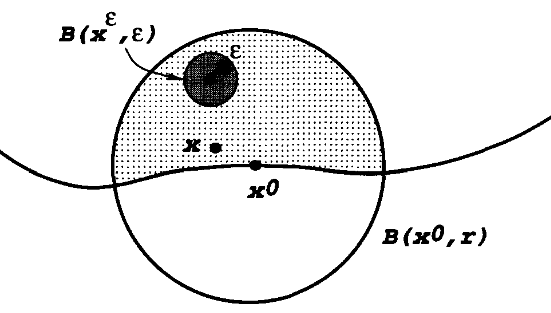
\includegraphics[width=0.5\textwidth]{Imagens/SobolevAproximaçãoGlobal.png}
\end{center}


2. Agora, seja \( u_\e(x) := u(x_\e) = u(x + \lambda\e e_n ) \) (\( x \in V \)). É a função \( u \) transladada. Ou seja, podemos pegar qualquer valor de \( x \in V \), e vamos calcular a \( u \) com o valor de um ponto mais pra cima, que esteja com uma bolinha dentro de \( U \cap B(p,r) \), conforme a explicação acima.

Seja \( v_\e :=  \eta_\e * u_\e \). Movemos a \( u \) pra cima, conforme escrito, e agora podemos molificá-la.\begin{align*}
	v_\e(x) &= \int_U \eta_\e(y) u_\e (x-y)\ dy\\
	&= \int_{B(0,\e)} \eta_\e(y) u(x_\e -y)\ dy
\end{align*}

Basicamente, vamos usar várias funções transladadas e molificadas assim, com partições da unidade, para construir a aproximação. Então, \( v_\e \in C^\infty(\overline{V}) \)

Isso porque a $u_\e$ não está definida apenas em $V$, o que faria a molificação $ C^\infty $ apenas em $V_\e$. Na verdade, para $\e$ pequeno, ela está definida em qualquer conjunto contido em $\overline{U} \cap B(p,r)$. Então, por exemplo, podemos definir a $u_\e$ em $V_2  = \overline{U} \cap B(p, 3r/4)$ e a molificação será $C^\infty(X \subset\subset V_2) \Rightarrow C^\infty(V)$.

 Isso é porque é possível pegar valores na borda de \( V \) (borda de \( U \)) e ainda assim a função estar definida porque transladamos pra cima? .

3. Agora, provamos que \( v_\e \rightarrow u \) em \( W^{k,p}(V) \). Para isso, seja\( |\alpha| \leq k \). Então, \[ ||D^\alpha v_\e - D^\alpha u||_{L^p(V)} \leq ||D^\alpha v_\e - D^\alpha u_\e||_{L^p(V)} + ||D^\alpha u_\e - D^\alpha u||_{L^p} \] O segundo termo vai pra zero com \( \e \) porque a translação é contínua na norma \( L^p \). O primeiro vai pra zero porque é uma aproximação local (teorema de antes) em \( L^p_{loc}(U) \Rightarrow L^p(V)  \).

4. Seja \( \delta >0 \). Como \( \pu \) é compacto (porque \( U \) é limitado, ou por que \( \pu \in C^1 \)?), podemos encontrar finitos \( p_i \in \pu \), com \( r_i>0 \), conjuntos \( V_i = U \cap B(p_i, r_i/2) \) e funções \( v_i \in C^\infty(\overline{V_i}) \) tal que a união das bolas \( B(p_i, r_i/2) \) dê a fronteira \( \pu \) e também \[ ||v_i - u||_{W^{k,p}(V_i)}\leq \delta \] Seja um conjunto aberto \( V_0 \subset\subset U \) tal que \( U \subset \bigcup_{i=0}^N V_i \) e escolha, usando o teorema da aproximação local, uma função \( v_0 \in C^\infty (\overline{V_0}) \) tal que ela aproxime \( u \) dentro de \( V_0 \).

5. Seja \( \{ \zeta_i \}_{i=0}^N \) uma partição suave da unidade subordinada aos conjuntos abertos \( \{V_i\}_{i=0}^N \). Seja \( v:= \sum \zeta_i v_i \). Então, \( v \in C^\infty (\overline{U}) \). Como \( u = \sum \zeta_i u \), para cada \( |\alpha|\leq k \), \begin{align*}
	||D^\alpha v - D^\alpha u||_{L^p(U)} &\leq \sum_{i=0}^{N} || D^\alpha (\zeta_i v_i) - D^\alpha (\zeta_i u)||_{L^p(V_i)}\\
	&\leq C \sum_{i=0}^N ||v_i - u||_{W^{k,p}(V_i)} = CN\delta \rightarrow 0
\end{align*}

A primeira desigualdade decorre da desigualdade triangular. A segunda desigualdade decorre da propriedade (iv), a fórmula de Leibniz, a regra do produto. Ao fazê-la com $D^\alpha(\zeta_i f)$, ficaremos com $||(D^\alpha\zeta_i v_i - D^\alpha\zeta_i u) + \ldots + (\zeta_i D^\alpha v_i - \zeta_i D^\alpha u) ||$. Assim, como $\zeta_i$ é contínua com suporte compacto e logo limitada, podemos pegar o máximo dos valores $\zeta_i, \ldots, D^\alpha\zeta_i$, como $C$. Com a soma dessas diferenças $v_i - u$ com as várias derivadas dentro da norma $L^p$, por desigualdade triangular novamente, chegamos na norma de Sobolev. \qed

\subsection*{Resumo das Aproximações}

\begin{tabular}{cccc}
	\hline
	Tipo de aproximação & Espaço de convergência & \( \{u_m\} \)  & \( u_m \) \\
	\hline
	Aproximação interior	& \( W^{k,p}_{loc}(U) \) 	& \( u_m \in C^\infty(U_\e) \) & \( u_\e = \eta_\e * u \)\\
	
	Aproximação    			& \( \sobolevdef \) 		& \( u_m \in C^\infty(U)  \) & \( u_i = \sum \eta_{\e_i} * (\zeta_i u) \) \\
	
	Aproximação global	 	& \( \sobolevdef\), $ \pu $ é $ C^1 $		& \( u_m \in C^\infty(\overline{U}) \) &  \\
	\hline
\end{tabular}





\section{Extensões}

\paragraph{Teorema da Extensão} Seja \( U \) limitado e \( \pu \) seja \( C^1 \).  Escolha um conjunto aberto e limitado \( V \) tal que \( U \subset\subset V \). Então, existe um operador linear limitado \[ E:W^{1,p}(U) \rightarrow W^{1,p}(\Rn) \] tal que para cada \( u \in W^{1,p}(U) \) \begin{enumerate}[(i)]
	\item \( Eu=u \) q.t.p em \( U \)
	\item \( Eu \) tem suporte em \( V \)
	\item \[ ||Eu||_{W^{1,p}(\Rn)} \leq C ||u||_{W^{1,p}(U)} \] com uma constante \( C \) dependendo apenas de \( p, U, V \). \footnote{definição de operador limitado.}
\end{enumerate}

\textit{Demonstração.} Seja \( p \in \pu \) e suponha que \( \pu \) é plana (reta) perto de \( p \), estando no plano \( p_n=0 \). Então, podemos assumir que existe uma bola aberta \( B \) com centro \( p \) e raio \( r \) tal que \[ \begin{cases}
	B^+ := B \cap \{ p_n \geq 0 \}  \subset \overline{U}\\
	B^- := B \cap \{ p_n \leq 0 \} \subset \Rn - U 
\end{cases} \]

Assuma que \( u \in C^\infty (\overline{U}) \) (vamos usar as aproximações da seção anterior). Defina então \[ \overline{u}(x) := \begin{cases}
	u(x) & x \in B^+ \\
	-3u(x_1, \ldots, -x_n) + 4u(x_1, \ldots, -\frac{x_n}{2}) & x \in B^-
\end{cases} \] Podemos ver que ela é contínua na borda \( x \in B^+ \cup B^- \). Seja \( u^- := \overline{u}\mid_{B^-} \) e \( u^+ := \overline{u}\mid_{B^+} \).  Podemos ver que \( u^- = u^+ \) em \( \{x_n=0\}\). Além disso, as derivadas são iguais. Para \( u^-_{x_i} \) com \( i \neq n \), vem de que \( -3 + 4 = 1 \). Para \( u^-{x_n} \), é porque \( -3 \cdot (-1) + 4 \cdot \frac{-1}{2} = 1 \). Então, \( D^\alpha u^- = D^\alpha u^+ \) em \( \{x_n=0\} \).

Não poderíamos usar, como $ u^- $, apenas $ u(x) $ pois ela não estaria definida, e nem $ u(x_1,\ldots, -x_n) $ pois não teria a mesma derivada. A solução com os coeficientes acima é genial.


Enfim, $ \overline{u} $ é contínua com derivadas contínuas, então \[ \overline{u} \in C^1(B) \]
Com esses cálculos, podemos verificar que \[ ||\overline{u}||_{W^{1,p}(B)} \leq C ||u||_{W^{1,p}(B^+)} \] com uma constante \( C \) que não depende de \( u \). $\overline{u} $ está limitada por $u$ pois ela está definida a partir de $u$, então a relação faz sentido. Por exemplo, $|\overline{u}| \leq 10  |u| $.

Caso \( \pu \) não seja plana perto de \( p \), podemos planificar a borda com uma função \( \Phi \in C^1 \) com inversa \( \Psi \) tal que \( \Phi \) planifique a borda perto de \( p \).
\( \Phi: x \rightarrow y \) em que nas variáveis \( y \) a borda é planificada. Seja \( u'(y) := u(\Psi(y)) \) (para calcular a função em \( y \), encontre o \( x \) correspondente). Aí, fazemos a mesma coisa que anteriormente. Então \[ ||\overline{u}'||_{W^{1,p}(B)} \leq C ||u'||_{W^{1,p}(B^+)} \]

Seja \( W:= \Psi(B) \) (os pontos \( x \) correspondentes à bola \( B \)). Convertendo de volta para variáveis \( x \), temos a extensão \( \overline{u} \) de \( u \) para \( W \), com \[ ||\overline{u}||_{W^{1,p}(W)} \leq C ||u||_{W^{1,p}(U)} \] Podemos majorar o lado direito pois \( \Psi(B^+) \subset  U  \).

Como \( \pu \) é compacto, existem finitos pontos \( p_i \in \pu \), conjuntos abertos \( W_i \), e extensões \( \overline{u}_i \) de \( u \) para \( W_i \), conforme acima, tal que \( \pu \subset \bigcup_{i=1}^N W_i \). Seja \( W_0 \subset\subset U \) tal que \( U \subset \bigcup_{i=0}^N W_i \), e seja \( \{ \zeta_i \} \) uma associada partição da unidade.

Seja \( \overline{u} := \sum_{i=0}^{N} \zeta_i \overline{u}_i \) com \( \overline{u}_0 = u \).  Utilizando a estimativa acima, com \( \overline{u}_i \) e \( u_i \), temos que \[ ||\overline{u}||_{W^{1,p}(\Rn)} \leq C ||u||_{W^{1,p}(U)} \]
para uma constante \( C \) que dependa de \( U,p,n \) mas não de \( u \). Além disso, podemos ajustar o suporte de \( \overline{u} \) para caber em \( V \supset\supset U \).

Por fim, escrevemos \( Eu:=\overline{u} \) e vemos que o operador é linear. 

A construção assumiu que \( u \in C^\infty(\overline{U}) \). Suponha agora que \( u \in W^{1,p}(U) \) e escolha \( u_m \in C^\infty(\overline{U}) \) como aproximação (podemos fazer isso já que \( \pu  \) é \( C^1 \)). O operador é linear e limitado, então \( Eu_m \rightarrow Eu \) é uma sequência de Cauchy convergente. \qed

\paragraph{Observação.} Embora $ \overline{u} $ não seja $ C^2 $, ela é $ W^{2,p}(B) $ (Ela não tem segunda derivada no sentido clássico, mas tem derivada fraca). Aí então, podemos usar o mesmo operador linear para fazer uma extensão, exatamente da mesma forma, de $ W^{2,p}(U) $ para $ W^{2,p}(\Rn) $.

Por outro lado, esse método não funciona para $ W^{k,p} $ com $ k>2 $.




\section{Traços}

Vamos agora assinalar valores de borda para uma função $u \in W^{1,p}(U)$, assumindo que $\pu$ é $C^1$. Se $u \in C(\overline{U})$, ela já tem valores de borda no sentido clássico. Porém, normalmente uma função em $W^{1,p}(U)$ não é contínua, e às vezes só é definida q.t.p em $U$. 

Como a borda tem medida n-dimensional de Lebesgue nula, não há sentido em dizer '$ u $ restrita a $ \pu $'. \textbf{???}





\paragraph{Teorema dos traços} Seja $U$ limitado e $\pu$ sendo $C^1$. Então, existe um operador linear e limitado \[ T:W^{1,p}(U)\rightarrow L^p(\pu) \] tal que \begin{enumerate}[(i)]
	\item $Tu = u$ em $\pu$ se $u \in W^{1,p}(U) \cap C(\overline{U})$
	\item \[ || Tu ||_{L^p(\pu)} \leq C ||u||_{W^{1,p}(U)} \] com uma constante que depende apenas de $p$ e $U$ (definição de operador limitado)
\end{enumerate} $Tu$ é chamado de traço de $u$ em $\pu$.

\textit{Demonstração.} 1. Suponha que $u \in C^1(\overline{U})$. Assim como na demonstração anterior, seja $p \in \pu$ e seja $\pu$ plano no entorno de $p$, estando no plano $\{x_n=0\}$. Seja $B$ uma bola aberta da mesma forma que anteriormente, e $\hat{B}$ a bola concêntrica de raio $r/2$.

Escolha $\zeta \in C^\infty_c(B)$ com $\zeta\geq0$ em $B$, e com $\zeta\equiv1$ (identicamente 1) em $\hat{B}$. Seja $\Gamma$ a parte de $\pu$ contida em $\hat{B}$. Seja $x'=(x_1, \ldots, x_{n-1}) \in \R^{n-1}= \{x_n=0\}$.

\begin{center}
	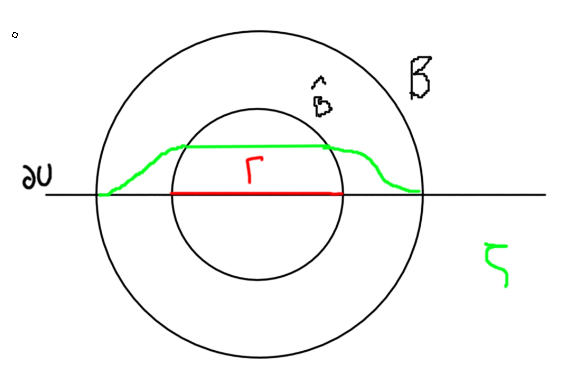
\includegraphics[width=0.5\textwidth]{Imagens/Sobolev-5}
\end{center}

Aí, \[
	\int_\Gamma |u|^p dx' = \int_\Gamma 1|u|^p dx' = \int_\Gamma \zeta |u|^p dx' \leq \int_{\{x_n=0\}} \zeta |u|^p dx'
\] aí, pelo teorema de Gauss-Green $ \int_U u_{x_i}\ dx = \int_{\partial U} u \vec{\nu_i}\ dS $, \[ \int_{\{x_n=0\}} \zeta |u|^p\ dx' = -\int_{B^+} \left(\zeta |u|^p \right)_{x_n}\ dx \] porque o vetor normal apontando pra fora de $B^+$ aponta pra baixo. Tirando a derivada, \[ = -\int_{B^+} |u|^p \zeta_{x_n} + p |u|^{p-1} (\text{sgn } u) u_{x_n} \zeta\ dx \]
Pela desigualdade de Young para produtos, podemos majorar o segundo termo \[ \left| p  |u|^{p-1} (\text{sgn } u ) u_{x_n} \zeta \right| \leq |u|^{p-1} |Du| \leq \frac{1}{p'}(|u|^{p-1})^{p'} + \frac{1}{p}|Du|^p \leq C\left( |u|^p + |Du|^p\right)\] ficamos com \[ \leq C \int_{B^+} |u|^p + |Du|^p\ dx \]

2.

Se $p \in \pu$ mas $\pu$ não é plana no entorno de $p$, como sempre iremos planificar a borda.

Aplicando a estimativa acima e mudando variáveis, ficamos com \[ \int_\Gamma |u|^p\ dS \leq C \int_U |u|^p + |Du|^p\ dx \] em que $\Gamma \subset \pu$ aberto contendo $p$. Elevado a $ \frac{1}{p} $ dos dois lados, à esquerda ficamos com a norma $ L^p $ e à direita com a norma de Sobolev $ W^{1,p} $.

No lado direito seria uma forma de $\Psi(B^+)$, com $\Psi$ a função inversa da planificação. Podemos majorar para $U$ pois $B^+ \subset U$.

3.

Como $\pu$ é compacto, existem finitos pontos $p_i \in \pu$ e conjuntos abertos $\Gamma_i \subset \pu$ tal que $\pu = \bigcup_{i=1}^N \Gamma_i$ com \[ ||u||_{L^p(\Gamma_i)} \leq C ||u||_{W^{1,p}(U)} \] pela desigualdade anterior.

Se definirmos \[ Tu := u \text{ em } \pu \] então \[ ||Tu||_{L^p(\pu)} \leq C ||u||_{W^{1,p}(U)} \] com uma constante que não depende de $u$.


4.

A desigualdade do operador acima vale para $u \in C(\overline{U})$. Assuma agora que $u \in W^{1,p}(U)$. Então, existem funções $u_m \in C^\infty (\overline{U})$ que convergem para $u$ em $W^{1,p}(U)$. De acordo com a desigualdade acima, temos que se $u_m$ converge, então $Tu_m$ converge também. Definimos então \[ Tu := \lim_{m\rightarrow \infty} Tu_m \] 

Finalmente, se $u \in W^{1,p}(U) \cap C(\overline{U})$, percebemos que $u_m \in C^\infty(\overline{U})$ convergem uniformemente para $u$ em $\overline{U}$. Então $Tu=u$ em $\pu$.

\qed






\paragraph{Teorema do traço nulo} Seja $U$ limitado com $\pu$ $C^1$. Suponha que $u \in W^{1,p}(U)$. Então \[ u \in W^{1,p}_0(U) \Leftrightarrow Tu =0 \text{ em } \pu \]

\textit{Demonstração.} (ida) Suponha que $ u \in W^{1,p}_0(U) $. Então, por definição, existem funções $ u_m \in C^\infty_c(U) $ tal que $ u_m\rightarrow u $ em $ W^{1,p}(U) $. Como $ Tu_m=0 $ em $ \pu $ (pois para funções $ C(\overline{U}) $, $ Tu=u $ na borda) e $ T:W^{1,p}(U)\rightarrow L^p(\pu) $ é um operador linear e limitado, então $ Tu=0 $ em $ \pu $.

(volta) Seja $ Tu=0 \text{ em } \pu $. Usando partições da unidade e planificando $ \pu $, podemos assumir que \[ \begin{cases}
	u \in W^{1,p}(\R^n_+) \\
	u \text{ tem suporte compacto em } \overline{\R}^n_+\\
	Tu=0 \text{ em } \p\R^n_+ = \R^{n-1}
\end{cases} \] Ou seja, estamos transformando $ \pu $ em $ {x_n=0} $.

Como $ Tu=0 $ em $ \R^{n-1} $, existem funções $ u_m \in C^1(\overline{\R}^n_+) $ tal que (como $\pu$ é $C^1$, o teorema garante $C^\infty$ até a borda) \[ u_m \rightarrow u  \text{ em } W^{1,p}(\R^n_+)\] e \[ u_m |_{\R^{n-1}} = Tu_m  \rightarrow Tu =0  \text{ em } L^p(\R^{n-1})\] $ Tu_m=u_m $ pois $ u_m $ é definida na borda, e converge para zero pois $Tu=0$, e é no espaço $ L^p $ pois este é o espaço de $ Tu_m $.

Sendo $ x' \in \R^{n-1} $, $ x_n\geq0 $, temos que (usando o Teorema Fundamental do Cálculo) \[ \left| u_m(x', x_n) \right| \leq | u_m(x',0) | + \int_0^{x_n} |u_{m,x_n}(x',t)| \ dt   \] 

Vamos lembrar que \( (a+b)^p \leq 2^p (a^p + b^p) \). Com isso, vamos chamar \( 2^p \) de $C$, uma constante que depende de $p$. Então, ficamos com \begin{align*}
	\left| u_m(x', x_n) \right|^p &\leq C \left[ | u_m(x',0) |^p + \left( \int_0^{x_n} |u_{m,x_n}(x',t)| \ dt \right)^p \right] \\
	&\leq C \left[ | u_m(x',0) |^p + \left( \left(\int_0^{x_n} |u_{m,x_n}(x',t)|^p \ dt\right)^{\frac{1}{p}} \left(\int_0^{x_n}1^{p'}\ dt\right)^{\frac{1}{p'}}  \right)^p \right] \\
	&\leq C\left[ | u_m(x',0) |^p + x_n^{p-1} \int_0^{x_n} |Du_{m}(x',t)|^{p}\ dt \right]
\end{align*}



Então, integrando em $\R^{n-1}$, \[ \int_{\R^{n-1}} | u_m(x',x_n) |^p\ dx' \leq C \left(  \int_{\R^{n-1}} | u_m(x',0) |^p \ dx' + x_n^{p-1} \int_0^{x_n} \int_{\R^{n-1}} | Du_m(x',t)|^p\ dx' dt  \right)\]

Aí, lembrando que $ u_m |_{\R^{n-1}} = Tu_m \rightarrow Tu=0 \text{ em } L^p(\R^{n-1})$, ou seja, a norma $L^p$ de $u_m(x',x_n=0)$ vai pra zero, então, se $m \rightarrow \infty$ \[  \int_{\R^{n-1}} | u(x',x_n) |^p\ dx' \leq C  x_n^{p-1} \int_0^{x_n} \int_{\R^{n-1}} | Du(x',t)|^p\ dx' dt  \] para q.t.p, $x_n>0$.


Agora, seja $\zeta \in C^\infty_c(\R)$ satisfazendo \[ \zeta \equiv 1 \text{ em } [0,1], \qquad \zeta \equiv 0 \text{ em } \R^+ - [0,2], \qquad 0 \leq \zeta \leq 1 \] e definimos \[ \begin{cases}
	\zeta_m(x) := \zeta (mx_n) & x \in \R^n_+ \\
	w_m := u(x)(1 - \zeta_m)
\end{cases} \]

Então, caso $ 0 \leq mx_n \leq 1 \Rightarrow 0 \leq x_n \leq \frac{1}{m} $, $\quad \zeta_m(x)=1 \Rightarrow w_m=0$.

$ \zeta \neq 0  $ somente se $ 0 \leq x_n \leq 2/m $. Então, se $ m \rightarrow \infty $, então $\zeta_m(x) = 0 $ q.t.p.

Continuando, temos que \[ \begin{cases}
	w_{m,x_n}=u_{x_n}(1 - \zeta_m) - mu\zeta' \\
	D_{x'}w_m = D_{x'}u(1-\zeta_m)
\end{cases} \]

Consequentemente, \begin{align*}
	 \int_{\R^n_+} |Dw_m - Du|^p\ dx &\leq C \int_{\R^n_+} |\zeta_m|^p |Du|^p \ dx  \\
	  & +Cm^p \int_0^{2/m} \int_{\R^{n-1}} |u|^p \ dx'dt \\
	 =: A + B
\end{align*}

Isso porque \[ Dw_m - Du = \begin{bmatrix}
	w_{m, x_1} - u_{x_1} \\
		w_{m, x_2} - u_{x_2} \\
	\vdots \\
	w_{m, x_n} - u_{x_n}
\end{bmatrix}  - \begin{bmatrix}
- \zeta_m u_{x_1} \\
-\zeta_m u_{x_2} \\
\vdots \\
-\zeta_m u_{x_n} - mu\zeta'
\end{bmatrix}\] 

A $ \zeta' $ foi retirada da integral e deixada como uma constante, já que ela é $C^\infty_c$, é limitada com derivadas limitadas, dá para remover da integral.


Então $A\rightarrow 0$ se $m\rightarrow \infty$ pois $\zeta_m \rightarrow 0$ q.t.p.

Para o termo $B$, vamos usar uma desigualdade provada logo acima. \begin{align*}
	B &\leq C m^p \left(\int_0^{2/m} t^{p-1}\ dt\right)\left(\int_0^{2/m} \int_{\R^{n-1}} |Du|^p \ dx' dx_n\right) \\
	&\leq C \int_0^{2/m} \int_{\R^{n-1}} |Du|^p \ dx'dx_n \rightarrow 0 \text{ enquanto } m \rightarrow \infty
\end{align*}

Portanto, descobrimos que $ Dw_m \rightarrow Du \text{ em } L^{p}(\R^n_+)$. Como, pela definição de $w_m$, $w_m\rightarrow u \text{ em } L^p(\R^n_+)$, concluímos que \[ w_m \rightarrow u \text{ em } W^{1,p}(\R^n_+) \]

Agora, como $ w_m=0 $ se $ 0 < x_n < 1/m $, podemos molificar $ w_m $ para produzir funções $ u_m \in C^\infty_c(\R^n_+) $ tal que $ u_m \rightarrow u \text{ em } W^{1,p}(\R^n_+)$. Logo, $ u \in W^{1,p}_0 (\R^n_+) $

\qed

Molificação de $w_m$: \[ u_m(x) = \int_{\R^n_+} w_m(y) \eta(x-y)\ dy \] Como é uma molificação, então $u_m \in C^\infty({\R^n_+}_\e)$ Ou seja, só é $C^\infty$ para $x_n> \e$. Porém, como $w_m=0$ se $0 < y_n < 1/m$, então podemos definir $m=1/\e$, e teremos que $w_m=0$ se $0 < y_n < \e$. Ou seja, se $y_n \rightarrow 0$, então a função dará zero, o que garante que ela seja $C^\infty({\R^n_+})$ e não apenas $C^\infty({\R^n_+}_\e)$.



\section{Desigualdades}

Queremos responder a pergunta: Se uma função $ u $ está em $ W^{1,p}(U) $, ela automaticamente está em outros espaços de Sobolev? A resposta será sim, mas dependendo dos casos \begin{enumerate}[(i)]
	\item $ 1 \leq p < n $
	\item $ p = n $
	\item $ n < p \leq \infty $
\end{enumerate}

\subsection{Gagliardo-Nirenberg-Sobolev}

Aqui, vamos assumir que $ 1 \leq p < n $, o caso (i) das opções anteriores. Vamos, inicialmente, lidar com a estimativa \[ \nor{u}{L^q(\Rn)} \leq C \nor{Du}{L^p(\Rn)}\] para todas funções $ u \in C^\infty_c(\Rn) $, e para alguma $ C>0 $, $ 1 \leq q < \infty $.

Vamos fazer uma função escalada da $ u $, para encontrar a relação entre $ q $ e $ p $: Usando $ u_{\lambda}(x):=u(\lambda x) $, temos que \[ \nor{u_{\lambda}}{L^q(\Rn)} \leq C \nor{Du_\lambda}{L^p(\Rn)}\] Aí, podemos calcular \[ \int_\Rn |u_{\lambda}|^q\ dx =  \int_\Rn |u(\lambda x)|^q\ dx = \frac{1}{\lambda^n} \int_\Rn |u(y)|^q\ dy\] Da mesma forma para $ Du $, \[ \int_\Rn |Du_{\lambda}|^p\ dx =  \lambda^p \int_\Rn |Du(\lambda x)|^p\ dx = \frac{\lambda^p}{\lambda^n} \int_\Rn |Du(y)|^p\ dy\]

Combinando isso na desigualdade, encontramos que \[ \nor{u}{L^q(\Rn)} \leq C \lambda^{1 - \frac{n}{p} + \frac{n}{q} }\] Caso o expoente de $\lambda$ não dê zero, poderíamos encontrar uma contradição mandando-o para 0 ou $\infty$. Logo, para que não haja contradição $ q = \frac{np}{n-p} $

\paragraph{Definição do Conjugado de Sobolev} Se $ 1\leq p < n $, o conjugado de Sobolev de $p$ é \[ p^* := \frac{np}{n-p} \] Perceba que $ \frac{1}{p^*} = \frac{1}{p} - \frac{1}{n}, \qquad p^* > p $


\paragraph{Teorema 1 (Desigualdade de Gagliardo-Nirenberg-Sobolev)}\label{t:sobolev-ineq-t1} Seja $ 1 \leq p < n $. Existe uma constante $C$, dependendo apenas de $p$ e $n$, tal que \[ ||u||_{L^{p^*}(\Rn)} \leq C \left|\left|Du\right|\right|_{L^{p}(\Rn)} \] para toda $u \in C^1_c(\Rn)$

Realmente precisamos que $u$ tenha suporte compacto. Por exemplo, $u \equiv 1$ não satisfaz a desigualdade. Mas, a constante não depende do tamanho desse suporte.

\textit{Demonstração.} Seja $p=1$. Logo, $p^* = \frac{n}{n-1}$. Como $u$ tem suporte compacto, para cada $i=1,\ldots,n$ e $x \in \Rn$, temos que \[ u(x) = \int_{-\infty}^{x_i} u_{x_i}(x_1, \ldots, y_i, \ldots, x_n) \ dy_i\] pois o valor de $u$ em $x_i \rightarrow -\infty$ é zero. Portanto, \[ |u(x)| \leq \int_{-\infty}^{+\infty} \left| Du(x_1, \ldots, y_i, \ldots, x_n) \right|\ dy_i \quad (i=1, \ldots, n)\]

Consequentemente, multiplicando para $i=1, \ldots, n$, temos que \[ |u(x)|^{\frac{n}{n-1}} \leq \prod_{i=1}^{n} \left( \int_{-\infty}^{+\infty} |Du(x_1, \ldots, y_i, \ldots, x_n)| \ dy_i \right)^{\frac{1}{n-1}}  \]

Integrando em relação a $x_1$, \begin{align*}
	\int_{-\infty}^{+\infty} |u|^{\frac{n}{n-1}}\ dx_1 &\leq \int_{-\infty}^{+\infty} \prod_{i=1}^{n} \left( \int_{-\infty}^{+\infty} |Du|\ dy_i \right)^{\frac{1}{n-1}}\ dx_1 \\
	&= \left( \int_{-\infty}^{+\infty} |Du|\ dy_1 \right)^{\frac{1}{n-1}} \int_{-\infty}^{+\infty} \prod_{i=2}^{n} \left( \int_{-\infty}^{+\infty} |Du|\ dy_i \right)^{\frac{1}{n-1}}\ dx_1 \\
	&\leq \left( \int_{-\infty}^{+\infty} |Du|\ dy_1 \right)^{\frac{1}{n-1}}  \left( \prod_{i=2}^{n} \int_{-\infty}^{+\infty} \int_{-\infty}^{+\infty} |Du|\ dx_1 dy_i \right)^{\frac{1}{n-1}} 
\end{align*} com a última desigualdade surgindo da desigualdade geral de Hölder (desigualdade de Hölder para 3 ou mais funções). Ou seja, a integral em $U=\R$ do produto de $n-1$ funções menor-igual que o produto das normas $L^{n-1}(\R)$  de cada uma. O expoente $n-1$ da norma corta com o expoente já existente \( \frac{1}{n-1} \).

Continuando a integração em $x_2, x_3, \ldots, x_n$, o fator da esquerda vai recebendo $dy_2, dy_3, \ldots$, enquanto que o da direita vai diminuindo, chegando em 1, finalizando o produto em \begin{align*}
	\int_\Rn |u|^{\frac{n}{n-1}}\ dx &\leq \prod_{i=1}^{n} \left(  \int_{-\infty}^{+\infty} \cdots \int_{-\infty}^{+\infty} |Du|\ dx_1 \ldots dy_i \ldots dx_n \right)^{\frac{1}{n-1}}\\
		\int_\Rn |u|^{\frac{n}{n-1}}\ dx &= \left( \int_{\Rn} |Du|\ dx \right)^{\frac{n}{n-1}}
\end{align*}  

Essa é a estimativa para $p=1 \Rightarrow p^* = \frac{n}{n-1}$: \[ ||u||_{L^{p^*}(\Rn)} \leq ||Du||_{L^1(\Rn)} \]



Consideramos agora o caso em que $ 1 < p < n $. Aplicamos a estimativa para $p=1$ em $v:= |u|^\gamma$, em que $\gamma>1$ será escolhida tal que $ \frac{\gamma n}{n-1} = (\gamma -1 ) \frac{p}{p-1} $. Ou seja, $ \frac{\gamma n}{n-1} = \frac{np}{n-p} = p^*$. Logo, \begin{align*}
	\left(\int_\Rn |u|^{\frac{\gamma n}{n-1}}\ dx \right)^{\frac{n-1}{n}} &\leq \int_\Rn \left| D|u|^\gamma \right|\ dx = \gamma \int_\Rn |u|^{\gamma -1} |Du|\ dx \\
	&\leq \gamma \left(  \int_\Rn |u|^{(\gamma -1) \frac{p}{p-1}}\ dx \right)^{\frac{p-1}{p}} \left( \int_\Rn |Du|^p\ dx \right)^{\frac{1}{p}} \\
	\left(\int_\Rn |u|^{p^*}\ dx \right)^{\frac{1}{p^*}} &\leq C \left( \int_\Rn |Du|^p\ dx \right)^{\frac{1}{p}}
\end{align*}\qed


P.S.: Há que se fazer um pouco de álgebra para encontrar a parte final. Por exemplo, calcular que $ \frac{n-1}{n} - \frac{p-1}{p} = \frac{1}{p^*}$.



\paragraph{Teorema 2}\label{t:sobolev-ineq-t2}(estimativas para \( W^{1,p} \)) Seja \( 1\leq p < n \). Seja \(U\) aberto e limitado com \(\partial U\) sendo \(C^1\). Seja \(u \in W^{1,p}(U)\). Então, \(u \in L^{p^*}(U)\) com a estimativa \[ ||u||_{L^{p^*}(U)} \leq C ||u||_{W^{1,p}(U)} \] com uma constante \(C\) que só depende de \(p, n, U\).

\textit{Demonstração.} Como $\pu$ é $C^1$, existe uma extensão $Eu=\overline{u} \in W^{1,p}(\Rn)$, tal que $\overline{u}=u \text{ em } U$, e tal que $\overline{u}$ tem suporte compacto e $ \nor{\overline{u}}{W^{1,p}(\Rn)} \leq C \nor{u}{W^{1,p}(U)} $.

Pelos teoremas de aproximação, como $\overline{u}$ tem suporte compacto, fazendo a primeira aproximação (molificação), existem funções $ u_m \in C^\infty_c(\Rn) $ tal que \[ u_m \rightarrow \overline{u} \quad \text{ em } W^{1,p}(\Rn) \]

Agora, de acordo com o Teorema 1, como $u_m \in C^1_c(\Rn)$, então $ ||u_m - u_l||_{L^{p^*}(\Rn)} \leq C ||Du_m  - Du_l||_{L^p(\Rn)} $ para todo $m,l \geq 1$, já que toda sequência convergente é de Cauchy. Logo, \[ u_m \rightarrow \overline{u} \text{ em } L^{p^*}(\Rn) \]

Como o Teorema 1 também implica que $ ||u_m||_{L^{p^*}(\Rn)} \leq C ||Du_m||_{L^p(\Rn)} $, as duas convergências acima dão o limite \[ ||\overline{u}||_{L^{p^*}(\Rn)} \leq C ||D\overline{u}||_{L^{p}(\Rn)} \]

Essa desigualdade e as propriedades da extensão $Eu$ finalizam a demonstração, porque \begin{align*}
	 ||u||_{L^{p^*}(U)} = ||\overline{u}||_{L^{p^*}(U)} \leq ||\overline{u}||_{L^{p^*}(\Rn)} &\leq  C ||D\overline{u}||_{L^{p}(\Rn)} \\
	  ||u||_{L^{p^*}(U)}  &\leq  C ||D\overline{u}||_{L^{p}(\Rn)}
\end{align*}

Agora, como sabemos que \[ ||\overline{u}||_{W^{1,p}(\Rn)} = \left( \int_\Rn |\overline{u}|^p + |D\overline{u}|^p\ dx \right)^{1/p} \geq \left(\int_\Rn |D\overline{u}|^p\ dx \right)^{1/p} = ||D\overline{u}||_{L^p(\Rn)}\] Então, \begin{align*}
	 ||u||_{L^{p^*}(U)}  &\leq  C ||D\overline{u}||_{L^{p}(\Rn)} \\
	  &\leq  C ||\overline{u}||_{W^{1,p}(\Rn)} \\
	  &\leq   C \nor{u}{W^{1,p}(U)} 
\end{align*}\qed





\paragraph{Teorema 3 (Desigualdade de Poincaré)}\label{t:sobolev-ineq-t3} Estimativas para \( W^{1,p}_0, 1 \leq p < n\). Seja \(U\) aberto e limitado. Seja $u \in W^{1,p}_0(\mathbb{R}^n)$ para algum \(1 \leq p < n\). Então, temos que \[ ||u||_{L^q(U)} \leq C ||Du||_{L^p(U)} \] para todo \( q \in [1, p^*]\). 

\textit{Demonstração.} Como $u \in W^{1,p}_0(U)$, existem funções $u_m \in C^\infty_c(U)$ convergindo para $u$ em $ W^{1,p}(U)$. Extendemos cada função $u_m$ para ser 0 em $\Rn-\overline{U}$ e aplicamos o Teorema 1 para provar que \[ ||u||_{L^{p^*}(U)} \leq C ||Du||_{L^p(U)} \] Como $ |U| < \infty  $ (ver a parte I), \[ ||u||_{L^q(U)} \leq C||u||_{L^{p^*}(U)} \] se $1 \leq q \leq p^*$. \qed

Em decorrência da desigualdade de Poincaré, em $ W^{1,p}_0(U) $ a norma $ ||Du||_{L^p(U)} $ é equivalente a $ ||u||_{W^{1,p}}(U) $ se $U$ é limitado. Isso porque \begin{align*}
	 ||u||_{W^{1,p}(U)}^p &= \nor{u}{L^p(U)}^p + \nor{Du}{L^p(U)}^p \leq (C + 1) \nor{Du}{L^p(U)}^p \\
	 \nor{Du}{L^p(U)} \leq ||u||_{W^{1,p}(U)} &\leq C \nor{Du}{L^p(U)}
\end{align*}


\subsection{Morrey}

\paragraph{Teorema 4 (Desigualdade de Morrey)}\label{t:sobolev-ineq-t4} Seja \( n < p \leq \infty \). Então existe uma constante \( C\), dependendo apenas de \(n\) e \(p\), tal que \[ ||u||_{C^{0, \gamma}(\Rn)} \leq C ||u||_{W^{1,p}(\Rn)} \] para toda \( u \in C^1 (\Rn)\), com \[ \gamma := 1 - \frac{n}{p} \]

\textit{Demonstração.} Escolha qualquer bola $B(x,r) \subset \Rn$. Vamos provar que existe $ C(n) $ tal que \[ \frac{1}{|B|} \int_{B(x,r)} |u(y) - u(x)| \ dy \leq C \int_{B(x,r)}  \frac{|Du(y)|}{|y-x|^{n-1}}\ dy   \]

Fixe $w \in \p B(0,1)$. Então, se $0 < s < r$, \begin{align*}
	| u(x+sw) - u(x) | &= \left| \int_0^s \frac{d}{dt}u(x + tw)\ dt \right| \\
	&= \left| \int_0^s Du(x+tw)\cdot w \ dt\right| \\
	& \leq \int_0^s \left| Du(x+tw) \right| \ dt \qquad (|w|=1)
\end{align*} Então, integrando nos dois lados,
\begin{align*}
	\int_{\p B(0,1)} | u(x+sw) - u(x) |\ dS &\leq \int_0^s \int_{\p B(0,1)}  \left| Du(x+tw) \right| \ dS dt \\
	&= \int_0^s \int_{\p B(0,1)}  \left| Du(x+tw) \right| \frac{t^{n-1}}{t^{n-1}} \ dS dt 
\end{align*} Seja $y=x+tw$ tal que $t = |x-y|$. Para converter de coordenadas polares, vamos usar o $t^{n-1}$. Vamos lembrar que $\int_{\p B(0,t)}\ dS = n \alpha(n) t^{n-1} = \int_{\p B(0,1)} t^{n-1}\ dS$. Ou seja, vamos trocar a integral de $\p B(0,1)$ para $\p B(0,t)$. Desta forma, vamos conseguir a integral $B(0,s)$. No caso, como estamos fazendo $y=x+tw$, vamos trocar para $B(x,s)$. Então, \begin{align*}
\int_{\p B(0,1)} | u(x+sw) - u(x) |\ dS &\leq \int_{B(x,s)} \frac{|Du(y)|}{|x-y|^{n-1}}\ dy \\
&\leq \int_{B(x,r)} \frac{|Du(y)|}{|x-y|^{n-1}}\ dy \\
\int_0^r \int_{\p B(0,1)} | u(x+sw) - u(x) |\ dS \cdot s^{n-1}\ ds &\leq \int_0^r \int_{B(x,r)} \frac{|Du(y)|}{|x-y|^{n-1}}\ dy \cdot s^{n-1}\ ds\\
\int_0^r \int_{\p B(0,s)} | u(x+sw) - u(x) |\ dS ds &\leq \frac{r^n}{n} \int_{B(x,r)} \frac{|Du(y)|}{|x-y|^{n-1}}\ dy  \\
\int_{ B(x,r)} | u(y) - u(x) |\ dy &\leq \frac{r^n}{n} \int_{B(x,r)} \frac{|Du(y)|}{|x-y|^{n-1}}\ dy 
\end{align*}

Agora, fixe $x \in \Rn$. Então, \begin{align*}
	|u(x)| &  \leq \frac{1}{|B|}\int_{B(x,1)}|u(x) - u(y) + u(y)| \ dy \\
	  &\leq \frac{1}{|B|}\int_{B(x,1)} |u(x) - u(y)| \ dy + \frac{1}{|B|}\int_{B(x,1)}| u(y) |\ dy 
\end{align*}
Então, \begin{align*}
	|u(x)| &\leq \frac{1}{|B|}\int_{B(x,1)} |u(x) - u(y)| \ dy + \frac{1}{|B|}\int_{B(x,1)}| u(y) |\ dy \\
	&\leq C\int_{B(x,1)} \frac{|Du(y)|}{|x-y|^{n-1}}\ dy + C ||u||_{L^p(B(x,1))}
\end{align*}
Na primeira parcela utilizamos a desigualdade logo acima, na segunda parcela usamos desigualdade de Hölder em $|u(y)|$ com $p$ e $1$ com $p'$. Perceba que as constantes não dependem de $x$, apenas de $p, n$ e $U$.

Utilizando Hölder na primeira parcela e também que $B(x,1) \subset \Rn$, encontramos \[ |u(x)| \leq C \left(\int_\Rn |Du|^p \ dy \right)^{1/p}      \left(  \int_{B(x,1)} \frac{dy}{|x-y|^{(n-1)\frac{p}{p-1}}}  \right)^{\frac{p-1}{p}}      + C ||u||_{L^p(\Rn)} \] Agora, se $p>n$, significa que \begin{align*}	n &< p \\
	1 - \tfrac{1}{n} &< 1 - \tfrac{1}{p} \\
	\frac{n-1}{n} &< \frac{p-1}{p}	\\
	(n-1)\frac{p}{p-1} &< n
\end{align*} Logo, como $ \frac{1}{|x|^\alpha} $ é integrável em torno da origem se $\alpha<n$, então temos que \[ \left(  \int_{B(x,1)} \frac{dy}{|x-y|^{(n-1)\frac{p}{p-1}}}  \right)^{\frac{p-1}{p}}< \infty \]

Portanto, \begin{align*}
	|u(x)| &\leq C \left(\int_\Rn |Du|^p \ dy \right)^{1/p}          + C ||u||_{L^p(\Rn)} \\
	&\leq C ||u||_{W^{1,p}(\Rn)}
\end{align*}

Como $x \in \rn$ é arbitrário, a desigualdade recém demonstrada implica que \[ \sup_{\rn} |u| \leq C ||u||_{W^{1,p}(\rn)} \]



Seguindo, escolha dois pontos $x,y \in \rn$ e seja $r:= |x-y|$. Seja $W:= B(x,r) \cap B(y,r)$. Então, \[ |u(x) - u(y)| \leq \frac{1}{|W|}\int_W |u(x) -u(z)|\ dz + \frac{1}{|W|} \int_W |u(y) - u(z)| \ dz\]

Então, como $W \subset B(x,r)$, \[ \frac{1}{|W|} \int_W |u(x) - u(z)| \ dz \leq C \frac{1}{|B|} \int_{B(x,r)} |u(x) - u(z)|\ dz \] Agora, pela desigualdade $ \int_{ B(x,r)} | u(y) - u(x) |\ dy \leq \frac{r^n}{n} \int_{B(x,r)} \frac{|Du(y)|}{|x-y|^{n-1}}\ dy  $ e por Hölder, \begin{align*}
	 \frac{1}{|W|} \int_W |u(x) - u(z)| \ dz &\leq C \left(\int_{B(x,r)} |Du|^p \ dy \right)^{1/p}      \left(  \int_{B(x,r)} \frac{dy}{|x-y|^{(n-1)\frac{p}{p-1}}}  \right)^{\frac{p-1}{p}} \\
	 &\leq C \left( \frac{r^n}{r^{(n-1)\frac{p}{p-1}}}\right)^{\frac{p-1}{p}} ||Du||_{L^p(\rn)} \\
	 &= Cr^{1-\frac{n}{p}} ||Du||_{L^p(\rn)}
\end{align*} Porque \[ n\frac{p-1}{p} - (n-1) = \frac{np}{p} - \frac{n}{p} -n + 1 = 1 - \frac{n}{p}\]

Da mesma forma, \[ \frac{1}{|W|} \int_W |u(y) - u(z)| \ dz \leq C r^{1-\frac{n}{p}} ||Du||_{L^p(\rn)} \]

Então, \begin{align*}
	|u(x) - u(y)| &\leq \frac{1}{|W|}\int_W |u(x) -u(z)|\ dz + \frac{1}{|W|} \int_W |u(y) - u(z)| \ dz \\
	&\leq Cr^{1-\frac{n}{p}} ||Du||_{L^p(\rn)}\\
	&= C|x-y|^{1-\frac{n}{p}} ||Du||_{L^p(\rn)}
\end{align*} Portanto, \[ [u]_{C^{0, 1-n/p}(\rn)} = \sup_{x\neq y} \left\{ \frac{|u(x) - u(y)|}{|x-y|^{1-n/p}}\right\}   \leq C   ||Du||_{L^p(\rn)}    \]

Sendo $\gamma = 1 - n/p$, por fim, queremos chegar na norma de Hölder, que é $ ||u||_{C^{0,\gamma}(\overline{U})} := ||u||_{C(\overline{U})} + [u]_{C^{0,\gamma}(\overline{U})}  $. Logo, somamos $||u||_{C(\Rn)}$ nos dois lados da desigualdade acima e lembrando que \[ \sup_{\rn} |u| \leq C ||u||_{W^{1,p}(\rn)} \leq C ||u||_{L^p(\rn)}\] então

Logo, sendo $\gamma = 1 - n/p$ \begin{align*}
	[u]_{C^{0,\gamma}(\rn)}&\leq C ||Du||_{L^p(\rn)}  \\
	[u]_{C^{0,\gamma}(\rn)} + ||u||_{C(\rn)} &\leq C ||Du||_{L^p(\rn)} + ||u||_{C(\rn)} \\
	[u]_{C^{0,\gamma}(\rn)} + ||u||_{C(\rn)} &\leq C ||Du||_{L^p(\rn)} + C||u||_{L^p(\rn)} \\
	||u||_{C^{0,\gamma}(\rn)} & \leq C ||u||_{W^{1,p}(\rn)}
\end{align*}\qed

Na última parte, vamos lembrar que $ (a^p + b^p) \geq \frac{1}{2^p}(a+b)^p$, logo \begin{align*}
	||u||_{W^{1,p}}^p &= ||Du||_{L^p}^p + ||u||_{L^p}^p \\ &\geq C(||Du||_{L^p} + ||u||_{L^p}) ^p \\
	||u||_{W^{1,p}} &\geq C ||Du||_{L^p} + C ||u||_{L^p}
\end{align*}

Ou seja, devemos lembrar que $||u||_{W^{1,p}}$ é equivalente a $||u||_{L^p} + ||Du||_{L^p}$.


\paragraph{Definição} Dizemos que $u^*$ é uma versão de $u$ se $u=u^*$ q.t.p.


\paragraph{Teorema 5}\label{t:sobolev-ineq-t5} (Estimativa para \( W^{1,p}, n<p \)) Seja \(U\) aberto e limitado com borda \( C^1\). Seja \(  n<p \) e \(  u \in W^{1,p}(U)  \). Então, \(\exists u^* \in C^{0,\gamma}(\overline{U})\) com \( \gamma = 1 - \frac{n}{p}\) tal que \[ || u^* ||_{C^{0,\gamma}(\overline{U})} \leq C ||u||_{W^{1,p}(U)} \] com \(C\) dependendo apenas de \(p, n, U\).

Em decorrência do Teorema 5, sempre identificaremos uma função $u \in W^{1,p}(U), p>n,$ com sua versão contínua.

\textit{Demonstração.} Como $\pu$ é $C^1$, então existe uma extensão $Eu = \overline{u} \in W^{1,p}(\Rn)$ com as propriedades já especificadas. Como $\overline{u}$ tem suporte compacto, obtemos dos teoremas de aproximação que existem funções $ u_m \in C^\infty_c(\Rn) $ tal que \[ u_m \rightarrow \overline{u} \text{ em } W^{1,p}(\Rn) \]

De acordo com o \nameref{t:sobolev-ineq-t4}, com $\gamma = 1 - n/p$, como $u_m \in C^1$, \[ ||u_m - u_l||_{C^{0,\gamma}\prn} \leq C ||u_m - u_l||_{W^{1,p}\prn} \] para todo $l,m\geq1$.  Como $||u_m - u_l||_{W^{1,p}\prn} \rightarrow 0$ pois $u_m \rightarrow \overline{u}$, então $||u_m - u_l||_{C^{0,\gamma}\prn} \rightarrow 0$. Logo, existe um limite para $u_m$ com a norma $C^{0,\gamma}\prn$. Seja $u^*$ esse limite. Então, $\exists u^* \in C^{0,\gamma}\prn$ tal que \[ u_m \rightarrow u^* \text{ em }C^{0,\gamma}\prn  \]

Devido a essas duas aproximações, $u^* = \overline{u} \text{ q.t.p em } \Rn$.  Como $\overline{u}=u \text{ q.t.p em } \Rn$, então $u^* = u \text{ q.t.p em } U$.

O Teorema 4 também implica que $||u_m||_{C^{0,\gamma}\prn} \leq C ||u_m||_{W^{1,p}\prn}$, já que $u_m \in C^1$. Mandando $m \rightarrow \infty$ nesta desigualdade, temos que \begin{align*}
	 ||u^*||_{C^{0,\gamma}\prn} &\leq  C ||\overline{u}||_{W^{1,p}\prn}  \\
	  ||u^*||_{C^{0,\gamma}(\overline{U})}  \leq ||u^*||_{C^{0,\gamma}\prn} &\leq  C ||\overline{u}||_{W^{1,p}\prn} \leq C ||u||_{W^{1,p}(U)} \\
	  ||u^*||_{C^{0,\gamma}(\overline{U})}  &\leq C ||u||_{W^{1,p}(U)}
\end{align*}
\qed


\subsection{Desigualdades Gerais}

\paragraph{Teorema 6 (desigualdades gerais)} Seja $U$ aberto e limitado de borda $C^1$. Seja $u \in W^{k,p}(U)$

\begin{enumerate}[(i)]
	\item Se \[ k < \frac{n}{p} \] então \(u \in L^q(U) \) com \( \frac{1}{q} = \frac{1}{p} - \frac{k}{n}\) tal que \[ ||u||_{L^q(U)} \leq C ||u||_{W^{k,p}(U)} \]
	
	\item Se \[ k > \frac{n}{p} \] então \(u \in C^{k- \left[\frac{n}{p}\right] - 1, \gamma}(\overline{U})\) com \[ \gamma = \begin{cases}
		\left[\frac{n}{p}\right] + 1 - \frac{n}{p}, \text{ se } \frac{n}{p} \notin\Z \\
		\text{ qualquer positivo } < 1, \text{ se } \frac{n}{p} \in \Z
	\end{cases} \] tal que \[ ||u||_{C^{k- \left[\frac{n}{p}\right] - 1, \gamma}(\overline{U})} \leq C ||u||_{W^{k,p}(U)} \]
\end{enumerate}

O valor $ \left[\frac{n}{p}\right] $ é o valor inteiro de $n/p$. As constantes dependem apenas de $k,p,n,\gamma, U$.

Perceba que (i) é uma generalização do \nameref{t:sobolev-ineq-t2}, e (ii) é uma versão do \nameref{t:sobolev-ineq-t5}.

\textit{Demonstração.}\begin{enumerate}[(i)]
	\item Seja $k < \frac{n}{p}$. Então, \( p < \frac{n}{k} \) e podemos usar os teoremas que exigem $p<n$.
	
	Seja $\alpha, \beta, \gamma, \delta$ tal que $|\alpha|=k, |\beta|=k-1, |\gamma|=k-2, |\delta|=k-3$.
	
	Como $|\beta|=k-1$ então $D^\beta u \in W^{k - |\beta|,p}(U) = W^{1,p}(U)$. Logo, aplicando o \nameref{t:sobolev-ineq-t2} em $D^\beta u$ temos que  \begin{align*}
		||D^\beta u||_{L^{p^*}(U)} &\leq C || D^\beta u ||_{W^{1,p}(U)} \\ &= C\left( ||D^\beta u||^p + ||D(D^\beta u)||^p \right)^{1/p} \\
		&\leq C ||u||_{W^{k,p}(U)}
	\end{align*}
	
	Então, $u \in W^{k-1,p^*}(U) = W^{|\beta|, p^*}$ pois a relação acima vale para todo $|\beta|\leq k-1$, pois $ W^{k-1,p}, W^{k-2,p}, W^{k-3,p}, \ldots, W^{2,p} \subset W^{1,p} $.
	
	Então, pelo mesmo raciocínio de antes temos que $ D^\gamma u \in W^{|\beta| - |\gamma|,p^*} = W^{1,p^*} $. Então, aplicando o Teorema 2 em $D^\gamma u \in W^{1,p^*}(U)$ temos \begin{align*}
		||D^\gamma u||_{L^{p^{**}}(U)} &\leq C ||D^\gamma u ||_{W^{1,p^*}(U)} \\ &\leq C ||D(D^\gamma u)||_{L^{p^*}(U)}\\ &= C ||D^\beta u||_{L^{p^*}(U)}
	\end{align*}
	
	Então, continuamos descendo nas derivadas e encontrando que $u \in W^{k-2, p^{**}}$ com $\frac{1}{p^{**}} = \frac{1}{p^*} - \frac{1}{n} = \frac{1}{p} - \frac{2}{n}$ e assim por diante: \begin{align*}
		||D^\beta u||_{L^{p^*}(U)} &\leq C ||u||_{W^{k,p}(U)} & u \in W^{k-1,p^*}(U)\\
		||D^\gamma u||_{L^{p^{**}}(U)} &\leq C ||D^\beta u||_{L^{p^*}(U)} & u \in W^{k-2, p^{**}}(U) \\
		||D^\delta u||_{L^{p^{***}}(U)} &\leq C ||D^\gamma u||_{L^{p^{**}}(U)} & u \in W^{k-3, p^{***}}(U) \\
		\vdots &\leq \vdots \\
		||u||_{L^{p^{k*}}(U)} &\leq C ||u||_{W^{k,p}(U)} & u \in W^{0, p^{k*}(U)} = L^{p^{k*}}(U)  
	\end{align*}
	Em que $ p^{k*} $ é dado por $ \frac{1}{p^{k*}} = \frac{1}{p} - \frac{k}{n} $. 
	
	Vemos que $ \frac{1}{p^{(k-1)*}} = \frac{n-(k-1)p}{np} = \frac{\frac{n}{p} - k + 1}{n} > \frac{1}{n} \Rightarrow p^{(k-1)*} < n$, o que garante que podemos aplicar o \nameref{t:sobolev-ineq-t2} de $p$ até $p^{(k-1)*}$.
	
	\qed
	
	
	\item Seja $k > \frac{n}{p} \notin \Z$. Vamos supor que $\frac{n}{k} < p < n$. Depois, como $p^* > p$, podemos supor novamente que $\frac{n}{k} < p < p^* < n$. Em algum momento os $p^*$ passam $n$. Seja $l$ o número de $*$ de quando isso acontece, de quando $p^{l*}>n$. Aqui, paramos as desigualdades, pois $p^{(l+1)*}$ é negativo. Ou seja, vamos provar que $u \in W^{k-l,p^{l*}}(U)$ (até o primeiro $p^*$ que passa de $n$).
	
	Vejamos um exemplo: $n=12, p=5$ e $k=5$. Temos que $k>n/p$. Então \begin{align*}
		\frac{n}{k} < p &< n & 2\v4 < 5 < 12\\
		p < p^* &< n & p^* = 8\v57\ldots\\
		p < p^* &< n < p^{**} & p^{**} = 29\v98\ldots \\
		&& p^{***} < 0 
	\end{align*}

	Logo, podemos provar que $u \in W^{k-2, p^{**}}(U)$, aplicando o teorema em $p^*$ pois $p^* < n$. Ou seja $l=2$.
	
	No caso genérico, temos que encontrar o maior valor de $l$ tal que $p^{l*}>0$. Ou seja, encontrar $l$ tal que \[ \frac{1}{p^{l*}} = \frac{1}{p} - \frac{l}{n} > 0  \] Então, é necessário que $n - lp >0$. Então, vamos escolher o maior $l$ inteiro tal que \[ l < \frac{n}{p} \] Este $l$ será $l= \left[\frac{n}{p}\right]$, a parte inteira de $n/p$. No caso do nosso exemplo $l=\left[\frac{12}{5}\right] = \left[2\v 4\right] = 2$.
	
	Então, pelo raciocínio acima, usando o \nameref{t:sobolev-ineq-t2} temos que \[  u \in W^{k-l,r}(U)   \]com $ \frac{1}{r} = \frac{1}{p} - \frac{l}{n} $.
	
	Se $u \in W^{k-l. r}(U)$, então $D^\beta \in W^{1,r}(U)$ para $|\beta|\leq k-l-1$, porque \begin{align*}
		u \in W^{k-l,r}(U) &\Rightarrow u \in W^{1,r}(U)\\
		\vdots & \Rightarrow \vdots \\
		D^\beta u \in W^{1,r}(U) &\Rightarrow D^\beta u \in W^{1,r}(U) \\
		D^\alpha u \in W^{0,r}({U}) &\Rightarrow D^\alpha \in L^r 
	\end{align*}

	Então, aplicando o \nameref{t:sobolev-ineq-t5} em toda $D^\beta u$ com $|\beta|\leq k-l-1$, temos que $D^\beta u \in C^{0, 1 - \frac{n}{r}}(\overline{U})$, já que $r>n$. Outra interpretação é pensar que se a derivada fraca de uma função é contínua, a função é contínua.
	
	
	
	
	Logo, temos que \[ u \in C^{k-l-1, 1 - \frac{n}{r}}(\overline{U}) \]
	
	Agora, para simplificar, vemos que $ 1-\frac{n}{r} = 1 - \frac{n}{p} + l = \left[\frac{n}{p}\right] + 1 - \frac{n}{p}$ e que $ k-l-1 = k - \left[\frac{n}{p}\right] - 1$. Então, \[ u \in C^{k-\left[\frac{n}{p}\right]-1, \gamma}(\overline{U}) \] para $\gamma = \left[\frac{n}{p}\right] + 1 - \frac{n}{p}$, que é 1 menos a parte decimal de $n/p$.
	
	Para a estimativa da norma, sendo $\gamma = 1 - \frac{n}{r}$,
	\begin{align*}
		||u^*||_{C^{0,\gamma}(\overline{U})} &\leq C ||u||_{W^{1,r}(U)}  \leq C ||u||_{W^{k,p}(U)}\\
		\vdots & \leq \vdots \\
		||D^\beta u^*||_{C^{0,\gamma}(\overline{U})} &\leq C ||D^\beta u||_{W^{1,r}(U)} \leq C ||u||_{W^{k,p}(U)}
	\end{align*}

	Pela definição da norma de Hölder (soma das normas de Hölder para as derivadas). Então, ao somar as desigualdades acima, encontramos
	\[ ||u||_{C^{k-\left[\frac{n}{p}\right]-1, \gamma}(\overline{U})} \leq C ||u||_{W^{k,p}(U)} \]\qed
	
	
	
	\item Seja $k>\frac{n}{p} \in \Z$. Aqui, fazemos o mesmo raciocínio de antes, encontrando $l$ tal que $p^{l*}>n$. Porém, ao tentar fazer isso, encontraremos que $r:= p^{l*}=n$. Ou seja, $l = \left[\frac{n}{p}\right]-1 = \frac{n}{p}-1$. Logo, \[ u \in W^{k-l,n}(U) \]
	
	Então, $ D^\alpha u \in W^{k-l-|\alpha|,n}(U) $ para todo $k-l-|\alpha|\geq1 \Rightarrow k-l-1 \geq |\alpha|$. 
	
	Aí, então, pelo Teorema1,2,3? Temos que $D^\alpha u \in L^q(U)$ para todo $n\leq q < \infty$ \textbf{(??? isso porque $p^* = n^2/0$?)} com $|\alpha|\leq k-l-1 = k - \left[\frac{n}{p}\right]$. 
	
	Logo, $D^\beta u \in W^{1,q}(U)$ para todo $|\beta| \leq k - \left[\frac{n}{p}\right] - 1$, com $q$ tal que $n<q<\infty$. Então, pelo teorema \nameref{t:sobolev-ineq-t5}, $D^\beta u \in C^{0,1 - \frac{n}{q}}(U)$, com a relação \[ ||D^\beta u||_{C^{0,1 - \frac{n}{q}}(\overline{U})} \leq C ||D^\beta u||_{W^{1,q}(U)} \leq C ||u||_{W^{k-l,q}} \]
	
	Então, $ u \in C^{k-l-1,\gamma}(\overline{U}) $ com $\gamma = 1 - \frac{n}{q}$ em que $n < q < \infty$. Logo, $\gamma$ pode ser qualquer real entre 0 e 1. \qed
	
	
\end{enumerate}













\section{Compacidade}

Demonstramos recentemente que $W^{1,p}(U) \subset L^{p^*}(U)$ para $1 \leq p < n,\ p^* = \frac{np}{n-p}$. Vamos agora demonstrar que $W^{1,p}(U)$ está compactamente contido em $L^q(U)$ para $1 \leq q < p^*$. Essa compacidade será fundamental para as aplicações de análise funcional linear e não-linear para EDPs nos capítulos de 6 a 9.

\paragraph{Definição.} Sejam $X$ e $Y$ espaços de Banach, $X \subset Y$. Dizemos que $X$ está compactamente contido em $Y$, escrito $X \subset \subset Y$, se \begin{enumerate}[(i)]
	\item $ ||x||_Y \leq C ||x||_X $ para uma constante $C$, com $x \in X$.
	\item toda sequência limitada em $X$ é pré-compacta em $Y$.
\end{enumerate}
\href{https://en.wikipedia.org/wiki/Compact\_embedding}{Ver definição na Wikipédia.}

\paragraph{Teorema 1 (Rellich-Kondrachov)}\label{t:sobolev-compact} Seja \(U\) aberto e limitado com \(\partial U\) sendo \( C^1 \). Suponha \(1\leq p < n\). Então \[ W^{1,p}(U) \subset\subset L^q(U) \] para cada \(1 \leq q < p^* \).

\textit{Demonstração.} Fixe $1 \leq q < p^*$. Então, pelo \nameref{t:sobolev-ineq-t2} em \ref{t:sobolev-ineq-t2}, $W^{1,p}(U) \subset L^{p^*}(U)$. Porém, como $U$ é limitado, $L^{p^*}(U) \subset L^q(U)$ para $q<p^*$, por Hölder. Logo, \[ W^{1,p}(U) \subset L^q(U), \ ||u||_{L^q(U)} \leq C ||u||_{W^{1,p}(U)} \] 

Agora, resta provar que se $u_m$ é uma sequência limitada em $W^{1,p}(U)$, então existe uma subsequência $u_{m_j}$ que converge em $L^q(U)$.

Então, seja $\{u_m\}_{m=1}^\infty$ uma sequência limitada em $W^{1,p}(U)$. Ou seja, tal que $\sup_m ||u_m||_{W^{1,p}(U)} < \infty$.

Devido ao Teorema da Extensão, podemos supor sem perda de generalidade $U=\Rn$ e que as funções $\{u_m\}_{m=1}^\infty$ têm suporte compacto em $V \subset \Rn$. Podemos fazer isso pois duas funções iguais q.t.p. são elementos iguais em $W^{1,p}(U)$.

Primeiro, vamos analisar as funções suaves \[ u_m^\e := \eta_\e * u_m \] com $ \eta_\e $ o molificador padrão.  O suporte de $u_m^\e$ será a "soma"\ dos suportes de $\eta_\e$ (a bola $B(0,\e)$) com o de $u_m$ ($V$). Como $V$ não é muito importante, podemos aumentá-lo um pouco mais para que $\{u_m^\e\}$ tenham suporte compacto em $V$ também. Na verdade, uma solução melhor é pensar que dado um $\e$ pequeno, $u_m^\e$ terá suporte em $V$.

Agora, vamos demonstrar que \[ u_m^\e \rightarrow u_m \text{ em } L^q(V), \text{ uniformemente em } m\]

Para isso, sendo $u_m$ suave, \begin{align*}
	u_m^\e(x) - u_m(x) &= \int_{B(0,\e)} \eta_\e(y)u_m(x-y)\ dy\  -\  u_m(x)\\
	&= \int_{B(0,1)} \eta(y)\left(u_m(x-\e y) - u_m(x)\right)\ dy\\
	&=  \int_{B(0,1)} \eta(y) \int_0^1 \frac{d}{dt} (u_m(x-\e t y))\ dtdy \\
	&=  -\e \int_{B(0,1)} \eta(y) \int_0^1 Du_m(x - \e t y)\cdot y\ dtdy
\end{align*}
Agora, integrando em $\rn$ nos dois lados da equação, \begin{align*}
	\int_\Rn |	u_m^\e(x) - u_m(x) |\ dx &\leq \e  \int_{B(0,1)} \eta(y) \int_0^1 \int_\Rn  |Du_m(x - \e t y)|\ dx\ dt\ dy\\
	\int_V |	u_m^\e(x) - u_m(x) |\ dx &\leq \e  \int_{B(0,1)} \eta(y) \int_0^1 \int_V  |Du_m(z)|\ dz\ dt\ dy\\
	&\leq \e \int_V |Du_m(z)| \ dz
\end{align*}

O que provamos acima assume que $u_m$ é suave (a derivada utilizada
 é a clássica). Porém, pelos teoremas de aproximação, o acima é válido para $u_m \in W^{1,p}(V)$. Então, continuando,\[ 
	||u_m^\e - u_m||_{L^1(V)} \leq \e ||Du_m||_{L^1(V)} \leq \e C ||Du_m||_{L^p(V)} \leq \e C \]
A segunda desigualdade é válida pois $V$ é limitado, pois $||u||_{L^q(U)} \leq C ||u||_{L^p(U)}$ para $U$ limitado. Neste caso, usamos $q=1$. Esta desigualdade é normalmente utilizada para demonstrar que $L^p \subseteq L^q$, mas aqui utilizamos apenas a limitação. A última desigualdade decorre da hipótese de que $\{u_m\}$ é limitada.

Então, como a limitação não depende de $m$, \[ u_m^\e  \rightarrow u_m \text{ em } L^1(V), \text{ uniformemente em } m  \] 

Como $1 \leq q < p^*$, pela desigualdade de interpolação das normas $L^p$, temos que \[ ||u^\e_m - u_m||_{L^q(V)} \leq ||u^\e_m - u_m||^\theta_{L^1(V)} ||u^\e_m - u_m||^{1-\theta}_{L^{p^*}(V)} \] em que $ \frac{1}{q} = \frac{\theta}{1} + \frac{1-\theta}{p^*} $. Consequentemente, como a sequência está em $W^{1,p}(V)$, está em $L^{p^*}(V)$ por G-N-S, logo ela é limitada em $L^{p^*}$ e, então \[ ||u^\e_m - u_m||_{L^q(V)} \leq C ||u^\e_m - u_m||_{L^1(V)}^\theta \rightarrow 0 \]

Então, \( u_m^\e \rightarrow u_m \text{ em } L^q(V), \text{ uniformemente em } m\). Provamos que $\{u_m^\e\}_\e$ converge para $u_m$, mas ainda não provamos que $\{u_m\}$ converge em $L^q(V)$ (objetivo).

Agora, vamos provar que para cada $\e>0$ fixo, a sequência $\{u_m^\e\}_{m=1}^\infty$ é equilimitada (uniformemente limitada) e equicontínua. Ou seja, a sequência é feita variando $m$ e não $\e$. Para isto, vamos provar que a sequência é limitada por um valor que não depende de $m$ ou $x$, e suas derivadas são limitadas por um valor que não depende de $m$ ou $x$, assim a continuidade será feita utilizando-se da mesma constante.
\begin{align*}
	|u_m^\e(x)| &\leq \int_{B(x,\e)} \eta_\e(x-y)| u_m(y) |\ dy\\
	&\leq ||\eta_\e||_{ L^\infty(\Rn)} ||u_m||_{L^1(V) } \leq \frac{C}{\e^n} < \infty
\end{align*}
Utilizando Hölder, queremos demonstrar a desigualdade para todo $x$ e $\e$ fixos. Logo, em vez de $B(x,\e)$ usamos $\rn$. Como $u_m$ tem suporte compacto em $V$, fica $L^1(V)$ em vez de $L^1(\rn)$. Por fim, \[ ||\eta_\e||_{L^\infty(\rn)} =\left|\left|\frac{1}{\e^n} \eta\left(\frac{x}{\e}\right)\right|\right| = \frac{C}{\e^n} \] 

Da mesma forma, lembrando que $D\eta_\e(x) = \frac{1}{\e^n} D\eta(\frac{x}{\e}) \cdot \frac{1}{\e}$, 
\begin{align*}
	|Du_m^\e(x)| &\leq \int_{B(x,\e)} D\eta_\e(x-y)| u_m(y) |\ dy\\
	&\leq ||D\eta_\e||_{ L^\infty(\Rn)} ||u_m||_{L^1(V) } \leq \frac{C}{\e^{n+1}} < \infty 
\end{align*}
Logo, $\{u_m^\e\}_{m=1}^\infty$ é equilimitada e equicontínua. Agora precisamos mostrar que existe uma subsequência convergente em $L^q(V)$. Para isso, vamos lembrar que a sequência $\{u_m^\e\}_{m=1}^\infty$ possui suporte compacto em $V \subset \rn$, e é equilimitada e equicontínua. Logo, pelo teorema de Ascoli-Arzela, podemos obter uma subsequência $\{u_{m_j}^\e\}_{j=1}^\infty$ que converge uniformemente em $V$. Logo, \[
\lim_{j,k\rightarrow\infty} || u_{m_j}^\e - u_{m_k}^\e ||_{L^q(V)} = 0 \Rightarrow 	\limsup_{j,k\rightarrow\infty} || u_{m_j}^\e - u_{m_k}^\e ||_{L^q(V)} = 0 
\]

Agora, fixamos $\delta > 0$ e, como $u_m^\e \rightarrow u_m$ uniformemente em $L^q$, escolhemos $\e>0$ tal que, para todo $m$, \[ ||u_m^\e - u_m||_{L^q(V)} \leq \frac{\delta}{2} \]

Então, \begin{align*}
	|| u_{m_j} - u_{m_k} ||_{L^q(V)} &\leq || u_{m_j} - u_{m_j}^\e + u_{m_j}^\e -u_{m_k}^\e + u_{m_k}^\e -u_{m_k} ||_{L^q(V)} \\
	&\leq || u_{m_j} - u_{m_j}^\e || + || u_{m_j}^\e -u_{m_k}^\e || + || u_{m_k}^\e -u_{m_k} || \\
	&\leq \frac{\delta}{2} + || u_{m_j}^\e -u_{m_k}^\e || + \frac{\delta}{2} \\
	|| u_{m_j} - u_{m_k} ||_{L^q(V)} &\leq \delta + || u_{m_j}^\e -u_{m_k}^\e || \\
	\limsup_{j,k\rightarrow\infty} || u_{m_j} - u_{m_k} ||_{L^q(V)} &\leq \delta + 0 \leq \delta
\end{align*}
Não podemos usar o limite porque não sabemos se o limite estará definido no lado esquerdo. Provamos que a sequência de $\{u_m^\e\}$ é equilimitada e equicontínua, mas com a sequência $\{u_m\}$ não.

Agora, aplicamos um argumento tradicional de diagonalização. Dado $\delta=1$, encontramos uma subsequência $\{u_{m_j}\}$ tal que \[\limsup_{j,k\rightarrow\infty} || u_{m_j} - u_{m_k} ||_{L^q(V)} \leq 1 \qquad u_{m_1}, u_{m_2}, u_{m_3}\]

Não é possível garantir a convergência desta subsequência. Agora, tomamos ela como sequência original $\{u_m\}$, e fazesmo a mesma coisa, agora para $\delta=\frac{1}{2}$, e obtemos uma subsequência da subsequência anterior em que $\limsup \leq \delta/2$.

Fazemos isso infinitamente, e pegamos um elemento de cada subsequência. Lembrando que cada subsequência é subsequência da anterior. Pegamos o primeiro elemento tal que a norma da diferença entre este e os outros é $\leq \frac{\delta}{n}$. Assim, vamos conseguir uma subsequência (da 'diagonal') em que os temors ficam arbitrariamente próximos. Então, extraímos uma subsequência $\{u_{m_l}\}$ tal que \[ \limsup_{l,k\rightarrow\infty} ||u_{m_l} - u_{m_k}||_{L^q(V)} =0  \] 
\qed

\paragraph{Observação.} Como $p^*>p$ e $p^* \rightarrow \infty$ quando $p\rightarrow n$, então temos em particular \[W^{1,p}(U) \subset\subset L^p(U)\] para todo $1\leq p \leq \infty $. Observe que se $n < p \leq \infty$, então isso segue da desigualdade de Morrey e do teorema de Ascoli-Arzela. Primeiramente, sabemos que $W^{1,p}(U) \subset\subset L^p(U)$ para $1\leq p < n$ pela demonstração acima, já que $p^*>p$. Agora, se $p>n$, pelo \nameref{t:sobolev-ineq-t5}, sabemos que existe uma versão contínua $u^* \in C^{0, \gamma}(\overline{U})$, que, por ser contínua, está em $L^p(U)$. Agora, como provar que \[ ||u||_{L^p(U)} \leq C ||u||_{W^{1,p}(U)} \] \textbf{???}

Também veja que \[W^{1,p}_0(U) \subset\subset L^p(U)\] mesmo sem assumir que $\pu$ seja $C^1$.



\section{Tópicos Adicionais}

Até 5.8.3 em Janeiro.


\subsection{Desigualdades de Poincaré}

\paragraph{Teorema 1}\label{t:sobolev-poincare-t1} Seja \(U \subset \mathbb{R}^n \) limitado, conexo, com borda \(C^1\). Seja \(1 \leq p \leq \infty \). Então existe uma constante \(C\), dependendo apenas de \(n, p, U\) tal que \[ ||u- (u)_U ||_{L^p(U)} \leq C ||Du||_{L^p(U)} \] para cada função \(u \in W^{1,p}(U)\).

Notação: \((u)_U\) é a média de \(u\) em \(U\).

\section{Outros Espaços}

\section{Problemas}

\begin{enumerate}
	\item[18.] Use a transformada de Fourier para provar que se $u \in H^s(\Rn)$ para $s> n/2$, então $u \in L^{\infty}(\Rn)$ com a estimativa \[ ||u||_{L^\infty}(\Rn) \leq C ||u||_{H^s(\Rn)} \] em que $C$ só depende de $s,n$.
\end{enumerate}



































\end{document}
